%% 繁體中文譯本 / Traditional Chinese translation
%% 原文：Chen, D. (2026). Harmonicity accounts for the tritone's shortfall on the dissonance
%% curve for dyads.  原始碼：paper.tex（英文原版，保持不動）。
%% 本檔需以 XeLaTeX 編譯（xelatex paper_zh-TW.tex）；數值巨集 (numbers.tex)、
%% 表格內容 (tables_zh/) 與圖檔 (figures/) 與原文共用或同步譯出。
%%
%% 術語對照（首次出現處均附英文）：
%%  roughness 粗糙度；harmonicity 諧波度；consonance 協和；dissonance 不協和；
%%  tritone 三全音；dyad 二音組；partial 分音；pleasantness 愉悅度；
%%  held-out 留出；estimand 估計目標；noise ceiling 雜訊上限；sharpness 尖銳度；
%%  equal temperament 十二平均律；just intonation 純律；in-tune bonus 準音加成。
\documentclass[11pt,a4paper]{article}

\usepackage{fontspec}
\usepackage{xeCJK}
\usepackage{textcomp}
% 中文字型：依序嘗試常見的繁體中文字型（Noto／思源／Windows／macOS）
\IfFontExistsTF{Noto Serif CJK TC}{%
  \setCJKmainfont{Noto Serif CJK TC}[BoldFont={Noto Sans CJK TC Bold}]%
  \setCJKsansfont{Noto Sans CJK TC}%
  \setCJKmonofont{Noto Sans CJK TC}}{%
\IfFontExistsTF{Source Han Serif TC}{%
  \setCJKmainfont{Source Han Serif TC}\setCJKsansfont{Source Han Sans TC}\setCJKmonofont{Source Han Sans TC}}{%
\IfFontExistsTF{PMingLiU}{%
  \setCJKmainfont{PMingLiU}[BoldFont={Microsoft JhengHei}]\setCJKsansfont{Microsoft JhengHei}\setCJKmonofont{Microsoft JhengHei}}{%
\IfFontExistsTF{Songti TC}{%
  \setCJKmainfont{Songti TC}\setCJKsansfont{PingFang TC}\setCJKmonofont{PingFang TC}}{%
  \setCJKmainfont{Microsoft JhengHei}\setCJKsansfont{Microsoft JhengHei}\setCJKmonofont{Microsoft JhengHei}}}}}
\xeCJKsetup{CJKmath=true}
\renewcommand{\abstractname}{摘要}
\renewcommand{\refname}{參考文獻}
\renewcommand{\tablename}{表}
\renewcommand{\figurename}{圖}
% a true minus sign in text and in math (\textminus alone prints "=" in math mode; set at
% the start of the document, because hyperref redefines it there)
\AtBeginDocument{\DeclareRobustCommand{\textminus}{\ensuremath{-}}}
\usepackage[margin=2.5cm]{geometry}
\usepackage{amsmath,amssymb}
\usepackage{booktabs}
\usepackage{graphicx}
\usepackage{xcolor}
\usepackage[font=small,labelfont=bf,labelsep=quad]{caption}
\usepackage[authoryear,round]{natbib}
\usepackage{xr-hyper}
\usepackage[colorlinks=true,linkcolor=blue!50!black,citecolor=blue!50!black,urlcolor=blue!50!black]{hyperref}
\usepackage{microtype}
\usepackage{setspace}
% APA 7 引用格式：參考文獻 (bib_paper.tex) 由 analysis/apa_refs.py 產生；
% 兩位作者在敘述式引用中以「與」連接，在括號式引用中以「&」連接
\newif\ifapaparen
\DeclareRobustCommand{\apaand}{\ifapaparen\&\else\ 與\ \fi}
\NewCommandCopy{\natcitep}{\citep}
\RenewDocumentCommand{\citep}{o o m}{{\apaparentrue%
  \IfNoValueTF{#1}{\natcitep{#3}}{\IfNoValueTF{#2}{\natcitep[#1]{#3}}{\natcitep[#1][#2]{#3}}}}}
\setstretch{1.15}
\emergencystretch=2em
\setlength{\parindent}{2em}

% Every quoted result is a macro generated from the study's JSON outputs
% by analysis/make_tables.py; see the Code availability statement.
\newcommand{\sh}{\ensuremath{\sharp}}
\newcommand{\flip}[1]{\textbf{#1}}
% AUTO-GENERATED by analysis/make_tables.py -- do not edit by hand.
\newcommand{\ratingTT}{1.953}
\newcommand{\ratingMsix}{2.477}
\newcommand{\nBelowTT}{4}
\newcommand{\gapClarCFourS}{\textminus{}3.4}
\newcommand{\gapClarCFourSmin}{+6.8}
\newcommand{\gapClarCFourV}{+39.8}
\newcommand{\gapClarCFourHK}{\textminus{}46.6}
\newcommand{\gapBassoonHK}{+55.0}
\newcommand{\gapHornV}{+198.1}
\newcommand{\shareInstrAll}{26}
\newcommand{\shareModelAll}{16}
\newcommand{\shareInterAll}{58}
\newcommand{\shareInstrLRAll}{34}
\newcommand{\shareModelLRAll}{18}
\newcommand{\shareInterLRAll}{48}
\newcommand{\signModelAll}{11/48}
\newcommand{\signModelPctAll}{23}
\newcommand{\signInstrAll}{45/112}
\newcommand{\signInstrPctAll}{40}
\newcommand{\medRangeModelsAll}{34.6}
\newcommand{\medRangeInstrAll}{97.7}
\newcommand{\shareInstrNoV}{55}
\newcommand{\shareModelNoV}{8}
\newcommand{\shareInterNoV}{36}
\newcommand{\shareInstrLRNoV}{56}
\newcommand{\shareModelLRNoV}{11}
\newcommand{\shareInterLRNoV}{33}
\newcommand{\signModelNoV}{6/24}
\newcommand{\signModelPctNoV}{25}
\newcommand{\signInstrNoV}{38/84}
\newcommand{\signInstrPctNoV}{45}
\newcommand{\medRangeModelsNoV}{20.0}
\newcommand{\medRangeInstrNoV}{93.8}
\newcommand{\shareInstrRegAll}{26}
\newcommand{\shareModelRegAll}{36}
\newcommand{\shareInterRegAll}{38}
\newcommand{\shareInstrLRRegAll}{25}
\newcommand{\shareModelLRRegAll}{44}
\newcommand{\shareInterLRRegAll}{31}
\newcommand{\signModelRegAll}{20/54}
\newcommand{\signModelPctRegAll}{37}
\newcommand{\signInstrRegAll}{44/144}
\newcommand{\signInstrPctRegAll}{31}
\newcommand{\medRangeModelsRegAll}{53.8}
\newcommand{\medRangeInstrRegAll}{70.8}
\newcommand{\shareInstrRegNoV}{43}
\newcommand{\shareModelRegNoV}{30}
\newcommand{\shareInterRegNoV}{27}
\newcommand{\shareInstrLRRegNoV}{39}
\newcommand{\shareModelLRRegNoV}{34}
\newcommand{\shareInterLRRegNoV}{28}
\newcommand{\signModelRegNoV}{10/27}
\newcommand{\signModelPctRegNoV}{37}
\newcommand{\signInstrRegNoV}{44/108}
\newcommand{\signInstrPctRegNoV}{41}
\newcommand{\medRangeModelsRegNoV}{18.0}
\newcommand{\medRangeInstrRegNoV}{58.3}
\newcommand{\rangeClarKernels}{86.4}
\newcommand{\rangeHKInstr}{101.6}
\newcommand{\sensKernelMed}{18.0}
\newcommand{\sensKernelMax}{76.0}
\newcommand{\sensRecordingMed}{6.0}
\newcommand{\sensRecordingMax}{31.5}
\newcommand{\sensExtractionMed}{0.4}
\newcommand{\sensExtractionMax}{2.8}
\newcommand{\sensCodecMed}{0.3}
\newcommand{\sensCodecMax}{1.2}
\newcommand{\sensIdealMed}{8.8}
\newcommand{\sensIdealMax}{19.1}
\newcommand{\sensABWideMed}{39.4}
\newcommand{\sensABWideMax}{129.8}
\newcommand{\sensABNarrowMed}{13.9}
\newcommand{\sensABNarrowMax}{41.1}
\newcommand{\sensInstrMed}{93.8}
\newcommand{\sensInstrMax}{101.6}
\newcommand{\sensVassExtractMax}{168.3}
\newcommand{\sensVassExtractMed}{9.3}
\newcommand{\codecWorstVass}{3.6}
\newcommand{\codecWorstStable}{0.9}
\newcommand{\extrVassWorst}{134.1}
\newcommand{\extrHKWorst}{2.8}
\newcommand{\hornVassLoose}{+64.0}
\newcommand{\idealHKFlat}{\textminus{}3.2}
\newcommand{\idealHKBase}{+4.6}
\newcommand{\iowaHKDThree}{\textminus{}22.1}
\newcommand{\philHKDThree}{\textminus{}30.8}
\newcommand{\diffHKDThree}{8.7}
\newcommand{\eoIowaDThree}{0.405}
\newcommand{\eoPhilDThree}{0.487}
\newcommand{\iowaHKCFour}{\textminus{}43.0}
\newcommand{\philHKCFour}{\textminus{}46.6}
\newcommand{\diffHKCFour}{3.6}
\newcommand{\eoIowaCFour}{0.194}
\newcommand{\eoPhilCFour}{0.178}
\newcommand{\iowaHKCFive}{\textminus{}11.7}
\newcommand{\philHKCFive}{\textminus{}43.2}
\newcommand{\diffHKCFive}{31.5}
\newcommand{\eoIowaCFive}{0.347}
\newcommand{\eoPhilCFive}{0.089}
\newcommand{\sethCFiveIowa}{\textminus{}7.4}
\newcommand{\sethCFivePhil}{+15.3}
\newcommand{\mechHKpairShare}{70}
\newcommand{\mechHKpairBeat}{62}
\newcommand{\mechHKpairFlo}{1304}
\newcommand{\mechHKpairFhi}{1242}
\newcommand{\mechSethFundShare}{36}
\newcommand{\mechSethFundBeat}{108}
\newcommand{\mechFundCBW}{1.49}
\newcommand{\mechFundERB}{1.84}
\newcommand{\mechHKTTovMsix}{0.53}
\newcommand{\mechCelloFundShare}{73}
\newcommand{\abStableWide}{7}
\newcommand{\abStableNarrow}{11}
\newcommand{\abNSpectra}{17}
\newcommand{\abUnstableNarrow}{cello C3, cello C4, French horn C4, oboe C4, oboe C5, piano C4}
\newcommand{\cutCelloCFour}{+3.7}
\newcommand{\gapCelloCFourHK}{\textminus{}1.7}
\newcommand{\gapHornHK}{\textminus{}0.6}
\newcommand{\clarHKExtrMax}{1.5}
\newcommand{\clarCutMaxRange}{1.8}
\newcommand{\abUnstableMaxAbs}{11.7}
\newcommand{\abClarPositiveCells}{Philharmonia D3: $a=0.35, b=1$; Iowa D3: $a=0.35, b=1$, $a=0.35, b=1.5$}
\newcommand{\mechFundMean}{315}
\newcommand{\mechFundGpct}{0.17}
\newcommand{\erbSignChanges}{cello C4, oboe C4}
\newcommand{\erbNSignChanges}{2}
\newcommand{\pianoB}{3.17}
\newcommand{\pianoBse}{6.3}
\newcommand{\pianoResid}{0.005}
\newcommand{\pianoTopRatio}{15.52}
\newcommand{\vassExpSignChanges}{3}
\newcommand{\vassExpNSpectra}{17}
\newcommand{\abGridA}{0.15, 0.2, 0.25, 0.3, 0.35}
\newcommand{\abGridB}{1.0, 1.5, 2.0, 2.5, 3.0}
\newcommand{\hkGapRaw}{0.233}
\newcommand{\hkGapZ}{0.120}
\newcommand{\hkGapMean}{0.085}
\newcommand{\dRBRawI}{0.049}
\newcommand{\pRBRawI}{$p<.001$}
\newcommand{\dRBRawH}{0.010}
\newcommand{\pRBRawH}{$p=.004$}
\newcommand{\dRBRawF}{0.147}
\newcommand{\pRBRawF}{$p<.001$}
\newcommand{\RfullBRaw}{0.674}
\newcommand{\dRBSizeI}{0.075}
\newcommand{\pRBSizeI}{$p<.001$}
\newcommand{\dRBSizeH}{0.037}
\newcommand{\pRBSizeH}{$p<.001$}
\newcommand{\dRBSizeF}{0.080}
\newcommand{\pRBSizeF}{$p<.001$}
\newcommand{\RfullBSize}{0.738}
\newcommand{\dRBRegI}{0.085}
\newcommand{\pRBRegI}{$p<.001$}
\newcommand{\dRBRegH}{0.042}
\newcommand{\pRBRegH}{$p<.001$}
\newcommand{\dRBRegF}{0.058}
\newcommand{\pRBRegF}{$p<.001$}
\newcommand{\RfullBReg}{0.749}
\newcommand{\dRBTrI}{0.074}
\newcommand{\pRBTrI}{$p<.001$}
\newcommand{\dRBTrH}{0.043}
\newcommand{\pRBTrH}{$p<.001$}
\newcommand{\dRBTrF}{0.082}
\newcommand{\pRBTrF}{$p<.001$}
\newcommand{\RfullBTr}{0.737}
\newcommand{\rHKBRaw}{0.713}
\newcommand{\rankHKBRaw}{4}
\newcommand{\rHuronBRaw}{0.685}
\newcommand{\rankHuronBRaw}{5}
\newcommand{\rSethBRaw}{0.393}
\newcommand{\rankSethBRaw}{14}
\newcommand{\rVassBRaw}{0.389}
\newcommand{\rankVassBRaw}{15}
\newcommand{\rCorpusBRaw}{0.722}
\newcommand{\rankCorpusBRaw}{3}
\newcommand{\rStolzBRaw}{0.740}
\newcommand{\rankStolzBRaw}{2}
\newcommand{\rCompositeBRaw}{0.801}
\newcommand{\rankCompositeBRaw}{1}
\newcommand{\rHKBSize}{0.761}
\newcommand{\rankHKBSize}{3}
\newcommand{\rHuronBSize}{0.692}
\newcommand{\rankHuronBSize}{5}
\newcommand{\rSethBSize}{0.521}
\newcommand{\rankSethBSize}{12}
\newcommand{\rVassBSize}{0.455}
\newcommand{\rankVassBSize}{14}
\newcommand{\rCorpusBSize}{0.719}
\newcommand{\rankCorpusBSize}{4}
\newcommand{\rStolzBSize}{0.794}
\newcommand{\rankStolzBSize}{2}
\newcommand{\rCompositeBSize}{0.856}
\newcommand{\rankCompositeBSize}{1}
\newcommand{\rHKBReg}{0.771}
\newcommand{\rankHKBReg}{3}
\newcommand{\rHuronBReg}{0.706}
\newcommand{\rankHuronBReg}{5}
\newcommand{\rSethBReg}{0.540}
\newcommand{\rankSethBReg}{11}
\newcommand{\rVassBReg}{0.477}
\newcommand{\rankVassBReg}{14}
\newcommand{\rCorpusBReg}{0.722}
\newcommand{\rankCorpusBReg}{4}
\newcommand{\rStolzBReg}{0.796}
\newcommand{\rankStolzBReg}{2}
\newcommand{\rCompositeBReg}{0.857}
\newcommand{\rankCompositeBReg}{1}
\newcommand{\rHKBTr}{0.751}
\newcommand{\rankHKBTr}{3}
\newcommand{\rHuronBTr}{0.692}
\newcommand{\rankHuronBTr}{5}
\newcommand{\rSethBTr}{0.540}
\newcommand{\rankSethBTr}{12}
\newcommand{\rVassBTr}{0.453}
\newcommand{\rankVassBTr}{14}
\newcommand{\rCorpusBTr}{0.719}
\newcommand{\rankCorpusBTr}{4}
\newcommand{\rStolzBTr}{0.794}
\newcommand{\rankStolzBTr}{2}
\newcommand{\rCompositeBTr}{0.855}
\newcommand{\rankCompositeBTr}{1}
\newcommand{\dRJRawI}{0.005}
\newcommand{\pRJRawI}{$p=.344$}
\newcommand{\dRJRawH}{0.042}
\newcommand{\pRJRawH}{$p=.009$}
\newcommand{\dRJRawF}{0.141}
\newcommand{\pRJRawF}{$p<.001$}
\newcommand{\RfullJRaw}{0.414}
\newcommand{\dRJSizeI}{0.033}
\newcommand{\pRJSizeI}{$p=.013$}
\newcommand{\dRJSizeH}{0.100}
\newcommand{\pRJSizeH}{$p<.001$}
\newcommand{\dRJSizeF}{0.045}
\newcommand{\pRJSizeF}{$p=.004$}
\newcommand{\RfullJSize}{0.500}
\newcommand{\dRJRegI}{0.026}
\newcommand{\pRJRegI}{$p=.025$}
\newcommand{\dRJRegH}{0.108}
\newcommand{\pRJRegH}{$p<.001$}
\newcommand{\dRJRegF}{0.033}
\newcommand{\pRJRegF}{$p=.011$}
\newcommand{\RfullJReg}{0.516}
\newcommand{\dRJTrI}{0.068}
\newcommand{\pRJTrI}{$p<.001$}
\newcommand{\dRJTrH}{0.090}
\newcommand{\pRJTrH}{$p<.001$}
\newcommand{\dRJTrF}{0.031}
\newcommand{\pRJTrF}{$p=.012$}
\newcommand{\RfullJTr}{0.534}
\newcommand{\rHKJRaw}{0.440}
\newcommand{\rankHKJRaw}{8}
\newcommand{\rHuronJRaw}{0.680}
\newcommand{\rankHuronJRaw}{3}
\newcommand{\rSethJRaw}{0.065}
\newcommand{\rankSethJRaw}{13}
\newcommand{\rVassJRaw}{0.042}
\newcommand{\rankVassJRaw}{15}
\newcommand{\rCorpusJRaw}{0.568}
\newcommand{\rankCorpusJRaw}{5}
\newcommand{\rStolzJRaw}{0.723}
\newcommand{\rankStolzJRaw}{1}
\newcommand{\rCompositeJRaw}{0.628}
\newcommand{\rankCompositeJRaw}{4}
\newcommand{\rHKJSize}{0.529}
\newcommand{\rankHKJSize}{8}
\newcommand{\rHuronJSize}{0.682}
\newcommand{\rankHuronJSize}{4}
\newcommand{\rSethJSize}{0.171}
\newcommand{\rankSethJSize}{13}
\newcommand{\rVassJSize}{0.087}
\newcommand{\rankVassJSize}{14}
\newcommand{\rCorpusJSize}{0.568}
\newcommand{\rankCorpusJSize}{6}
\newcommand{\rStolzJSize}{0.783}
\newcommand{\rankStolzJSize}{1}
\newcommand{\rCompositeJSize}{0.694}
\newcommand{\rankCompositeJSize}{3}
\newcommand{\rHKJReg}{0.500}
\newcommand{\rankHKJReg}{9}
\newcommand{\rHuronJReg}{0.676}
\newcommand{\rankHuronJReg}{3}
\newcommand{\rSethJReg}{0.172}
\newcommand{\rankSethJReg}{12}
\newcommand{\rVassJReg}{0.026}
\newcommand{\rankVassJReg}{14}
\newcommand{\rCorpusJReg}{0.537}
\newcommand{\rankCorpusJReg}{7}
\newcommand{\rStolzJReg}{0.765}
\newcommand{\rankStolzJReg}{1}
\newcommand{\rCompositeJReg}{0.674}
\newcommand{\rankCompositeJReg}{4}
\newcommand{\rHKJTr}{0.594}
\newcommand{\rankHKJTr}{6}
\newcommand{\rHuronJTr}{0.682}
\newcommand{\rankHuronJTr}{4}
\newcommand{\rSethJTr}{0.428}
\newcommand{\rankSethJTr}{12}
\newcommand{\rVassJTr}{0.222}
\newcommand{\rankVassJTr}{13}
\newcommand{\rCorpusJTr}{0.568}
\newcommand{\rankCorpusJTr}{7}
\newcommand{\rStolzJTr}{0.783}
\newcommand{\rankStolzJTr}{1}
\newcommand{\rCompositeJTr}{0.716}
\newcommand{\rankCompositeJTr}{3}
\newcommand{\ratioFamIntBRaw}{3.0}
\newcommand{\ratioFamIntJRaw}{26}
\newcommand{\nHarm}{160}
\newcommand{\ntrialsHarm}{7{,}440}
\newcommand{\gapObsHarm}{+0.19}
\newcommand{\gapObsHarmCI}{[+0.04, +0.35]}
\newcommand{\gapHKHarm}{+0.18}
\newcommand{\gapHKHarmCI}{[+0.03, +0.33]}
\newcommand{\gapHKHHarm}{+0.12}
\newcommand{\gapHKHHarmCI}{[\textminus{}0.03, +0.28]}
\newcommand{\gapCompHarm}{+0.16}
\newcommand{\gapCompHarmCI}{[+0.01, +0.31]}
\newcommand{\gapSethHarm}{+0.18}
\newcommand{\gapSethHarmCI}{[+0.03, +0.33]}
\newcommand{\gapHHarm}{+0.10}
\newcommand{\gapHHarmCI}{[\textminus{}0.04, +0.26]}
\newcommand{\dipObsHarm}{+0.38}
\newcommand{\dipObsHarmCI}{[+0.25, +0.51]}
\newcommand{\dipHKHarm}{+0.29}
\newcommand{\dipHKHarmCI}{[+0.17, +0.42]}
\newcommand{\dipHKHHarm}{+0.10}
\newcommand{\dipHKHHarmCI}{[\textminus{}0.02, +0.22]}
\newcommand{\dipCompHarm}{+0.15}
\newcommand{\dipCompHarmCI}{[+0.03, +0.27]}
\newcommand{\dipSethHarm}{+0.34}
\newcommand{\dipSethHarmCI}{[+0.22, +0.47]}
\newcommand{\dipHHarm}{+0.08}
\newcommand{\dipHHarmCI}{[\textminus{}0.03, +0.19]}
\newcommand{\shareHKHarm}{5}
\newcommand{\rfitHKHarm}{0.22}
\newcommand{\shareHKHHarm}{38}
\newcommand{\rfitHKHHarm}{0.37}
\newcommand{\shareCompHarm}{17}
\newcommand{\rfitCompHarm}{0.35}
\newcommand{\shareHHarm}{46}
\newcommand{\rfitHHarm}{0.33}
\newcommand{\rawsdHarm}{1.31}
\newcommand{\nEqfive}{147}
\newcommand{\ntrialsEqfive}{11{,}754}
\newcommand{\gapObsEqfive}{+0.18}
\newcommand{\gapObsEqfiveCI}{[+0.07, +0.30]}
\newcommand{\gapHKEqfive}{+0.19}
\newcommand{\gapHKEqfiveCI}{[+0.07, +0.31]}
\newcommand{\gapHKHEqfive}{+0.04}
\newcommand{\gapHKHEqfiveCI}{[\textminus{}0.08, +0.16]}
\newcommand{\gapCompEqfive}{+0.05}
\newcommand{\gapCompEqfiveCI}{[\textminus{}0.06, +0.16]}
\newcommand{\gapSethEqfive}{+0.16}
\newcommand{\gapSethEqfiveCI}{[+0.05, +0.28]}
\newcommand{\gapHEqfive}{\textminus{}0.04}
\newcommand{\gapHEqfiveCI}{[\textminus{}0.16, +0.07]}
\newcommand{\dipObsEqfive}{+0.27}
\newcommand{\dipObsEqfiveCI}{[+0.14, +0.40]}
\newcommand{\dipHKEqfive}{+0.12}
\newcommand{\dipHKEqfiveCI}{[\textminus{}0.02, +0.24]}
\newcommand{\dipHKHEqfive}{\textminus{}0.09}
\newcommand{\dipHKHEqfiveCI}{[\textminus{}0.21, +0.04]}
\newcommand{\dipCompEqfive}{\textminus{}0.13}
\newcommand{\dipCompEqfiveCI}{[\textminus{}0.26, \textminus{}0.01]}
\newcommand{\dipSethEqfive}{+0.16}
\newcommand{\dipSethEqfiveCI}{[+0.03, +0.29]}
\newcommand{\dipHEqfive}{\textminus{}0.11}
\newcommand{\dipHEqfiveCI}{[\textminus{}0.23, +0.02]}
\newcommand{\shareHKEqfive}{-2}
\newcommand{\rfitHKEqfive}{0.52}
\newcommand{\shareHKHEqfive}{76}
\newcommand{\rfitHKHEqfive}{0.65}
\newcommand{\shareCompEqfive}{73}
\newcommand{\rfitCompEqfive}{0.69}
\newcommand{\shareHEqfive}{123}
\newcommand{\rfitHEqfive}{0.41}
\newcommand{\rawsdEqfive}{1.35}
\newcommand{\nNothree}{151}
\newcommand{\ntrialsNothree}{12{,}000}
\newcommand{\gapObsNothree}{+0.16}
\newcommand{\gapObsNothreeCI}{[+0.06, +0.26]}
\newcommand{\gapHKNothree}{+0.15}
\newcommand{\gapHKNothreeCI}{[+0.05, +0.25]}
\newcommand{\gapHKHNothree}{+0.01}
\newcommand{\gapHKHNothreeCI}{[\textminus{}0.10, +0.12]}
\newcommand{\gapCompNothree}{0.00}
\newcommand{\gapCompNothreeCI}{[\textminus{}0.10, +0.10]}
\newcommand{\gapSethNothree}{+0.13}
\newcommand{\gapSethNothreeCI}{[+0.03, +0.23]}
\newcommand{\gapHNothree}{\textminus{}0.08}
\newcommand{\gapHNothreeCI}{[\textminus{}0.18, +0.03]}
\newcommand{\dipObsNothree}{+0.23}
\newcommand{\dipObsNothreeCI}{[+0.14, +0.33]}
\newcommand{\dipHKNothree}{+0.28}
\newcommand{\dipHKNothreeCI}{[+0.19, +0.38]}
\newcommand{\dipHKHNothree}{+0.23}
\newcommand{\dipHKHNothreeCI}{[+0.14, +0.32]}
\newcommand{\dipCompNothree}{+0.21}
\newcommand{\dipCompNothreeCI}{[+0.12, +0.31]}
\newcommand{\dipSethNothree}{+0.28}
\newcommand{\dipSethNothreeCI}{[+0.18, +0.38]}
\newcommand{\dipHNothree}{+0.16}
\newcommand{\dipHNothreeCI}{[+0.07, +0.25]}
\newcommand{\shareHKNothree}{9}
\newcommand{\rfitHKNothree}{0.59}
\newcommand{\shareHKHNothree}{96}
\newcommand{\rfitHKHNothree}{0.70}
\newcommand{\shareCompNothree}{102}
\newcommand{\rfitCompNothree}{0.66}
\newcommand{\shareHNothree}{147}
\newcommand{\rfitHNothree}{0.33}
\newcommand{\rawsdNothree}{1.34}
\newcommand{\nFlute}{188}
\newcommand{\ntrialsFlute}{7{,}500}
\newcommand{\gapObsFlute}{+0.35}
\newcommand{\gapObsFluteCI}{[+0.22, +0.48]}
\newcommand{\gapHKFlute}{+0.36}
\newcommand{\gapHKFluteCI}{[+0.23, +0.50]}
\newcommand{\gapHKHFlute}{+0.34}
\newcommand{\gapHKHFluteCI}{[+0.20, +0.47]}
\newcommand{\gapCompFlute}{+0.27}
\newcommand{\gapCompFluteCI}{[+0.13, +0.40]}
\newcommand{\gapSethFlute}{+0.39}
\newcommand{\gapSethFluteCI}{[+0.26, +0.53]}
\newcommand{\gapHFlute}{+0.21}
\newcommand{\gapHFluteCI}{[+0.08, +0.35]}
\newcommand{\dipObsFlute}{+0.23}
\newcommand{\dipObsFluteCI}{[+0.11, +0.34]}
\newcommand{\dipHKFlute}{+0.10}
\newcommand{\dipHKFluteCI}{[\textminus{}0.02, +0.22]}
\newcommand{\dipHKHFlute}{+0.03}
\newcommand{\dipHKHFluteCI}{[\textminus{}0.09, +0.15]}
\newcommand{\dipCompFlute}{\textminus{}0.19}
\newcommand{\dipCompFluteCI}{[\textminus{}0.31, \textminus{}0.08]}
\newcommand{\dipSethFlute}{+0.14}
\newcommand{\dipSethFluteCI}{[+0.02, +0.25]}
\newcommand{\dipHFlute}{\textminus{}0.15}
\newcommand{\dipHFluteCI}{[\textminus{}0.27, \textminus{}0.03]}
\newcommand{\shareHKFlute}{-5}
\newcommand{\rfitHKFlute}{0.74}
\newcommand{\shareHKHFlute}{3}
\newcommand{\rfitHKHFlute}{0.75}
\newcommand{\shareCompFlute}{23}
\newcommand{\rfitCompFlute}{0.60}
\newcommand{\shareHFlute}{38}
\newcommand{\rfitHFlute}{0.21}
\newcommand{\rawsdFlute}{1.14}
\newcommand{\nGuitar}{186}
\newcommand{\ntrialsGuitar}{7{,}379}
\newcommand{\gapObsGuitar}{+0.39}
\newcommand{\gapObsGuitarCI}{[+0.25, +0.55]}
\newcommand{\gapHKGuitar}{+0.40}
\newcommand{\gapHKGuitarCI}{[+0.25, +0.55]}
\newcommand{\gapHKHGuitar}{+0.37}
\newcommand{\gapHKHGuitarCI}{[+0.23, +0.52]}
\newcommand{\gapCompGuitar}{+0.33}
\newcommand{\gapCompGuitarCI}{[+0.19, +0.48]}
\newcommand{\gapSethGuitar}{+0.38}
\newcommand{\gapSethGuitarCI}{[+0.24, +0.54]}
\newcommand{\gapHGuitar}{+0.30}
\newcommand{\gapHGuitarCI}{[+0.16, +0.44]}
\newcommand{\dipObsGuitar}{+0.33}
\newcommand{\dipObsGuitarCI}{[+0.20, +0.46]}
\newcommand{\dipHKGuitar}{+0.32}
\newcommand{\dipHKGuitarCI}{[+0.19, +0.45]}
\newcommand{\dipHKHGuitar}{+0.25}
\newcommand{\dipHKHGuitarCI}{[+0.12, +0.39]}
\newcommand{\dipCompGuitar}{+0.14}
\newcommand{\dipCompGuitarCI}{[+0.01, +0.27]}
\newcommand{\dipSethGuitar}{+0.35}
\newcommand{\dipSethGuitarCI}{[+0.22, +0.48]}
\newcommand{\dipHGuitar}{+0.09}
\newcommand{\dipHGuitarCI}{[\textminus{}0.04, +0.21]}
\newcommand{\shareHKGuitar}{-1}
\newcommand{\rfitHKGuitar}{0.86}
\newcommand{\shareHKHGuitar}{6}
\newcommand{\rfitHKHGuitar}{0.88}
\newcommand{\shareCompGuitar}{16}
\newcommand{\rfitCompGuitar}{0.69}
\newcommand{\shareHGuitar}{25}
\newcommand{\rfitHGuitar}{0.26}
\newcommand{\rawsdGuitar}{1.16}
\newcommand{\nPiano}{191}
\newcommand{\ntrialsPiano}{7{,}382}
\newcommand{\gapObsPiano}{+0.33}
\newcommand{\gapObsPianoCI}{[+0.18, +0.48]}
\newcommand{\gapHKPiano}{+0.32}
\newcommand{\gapHKPianoCI}{[+0.18, +0.48]}
\newcommand{\gapHKHPiano}{+0.29}
\newcommand{\gapHKHPianoCI}{[+0.15, +0.45]}
\newcommand{\gapCompPiano}{+0.25}
\newcommand{\gapCompPianoCI}{[+0.11, +0.40]}
\newcommand{\gapSethPiano}{+0.30}
\newcommand{\gapSethPianoCI}{[+0.16, +0.45]}
\newcommand{\gapHPiano}{+0.22}
\newcommand{\gapHPianoCI}{[+0.08, +0.37]}
\newcommand{\dipObsPiano}{+0.39}
\newcommand{\dipObsPianoCI}{[+0.27, +0.51]}
\newcommand{\dipHKPiano}{+0.36}
\newcommand{\dipHKPianoCI}{[+0.24, +0.48]}
\newcommand{\dipHKHPiano}{+0.28}
\newcommand{\dipHKHPianoCI}{[+0.17, +0.41]}
\newcommand{\dipCompPiano}{+0.13}
\newcommand{\dipCompPianoCI}{[+0.01, +0.25]}
\newcommand{\dipSethPiano}{+0.39}
\newcommand{\dipSethPianoCI}{[+0.28, +0.51]}
\newcommand{\dipHPiano}{+0.10}
\newcommand{\dipHPianoCI}{[\textminus{}0.02, +0.22]}
\newcommand{\shareHKPiano}{1}
\newcommand{\rfitHKPiano}{0.88}
\newcommand{\shareHKHPiano}{9}
\newcommand{\rfitHKHPiano}{0.90}
\newcommand{\shareCompPiano}{23}
\newcommand{\rfitCompPiano}{0.70}
\newcommand{\shareHPiano}{33}
\newcommand{\rfitHPiano}{0.27}
\newcommand{\rawsdPiano}{1.16}
\newcommand{\nPure}{151}
\newcommand{\ntrialsPure}{7{,}397}
\newcommand{\gapObsPure}{+0.21}
\newcommand{\gapObsPureCI}{[+0.08, +0.34]}
\newcommand{\gapHKPure}{+0.21}
\newcommand{\gapHKPureCI}{[+0.08, +0.34]}
\newcommand{\gapHKHPure}{+0.18}
\newcommand{\gapHKHPureCI}{[+0.05, +0.31]}
\newcommand{\gapCompPure}{+0.14}
\newcommand{\gapCompPureCI}{[+0.02, +0.26]}
\newcommand{\gapSethPure}{+0.15}
\newcommand{\gapSethPureCI}{[+0.03, +0.27]}
\newcommand{\gapHPure}{+0.15}
\newcommand{\gapHPureCI}{[+0.02, +0.27]}
\newcommand{\dipObsPure}{+0.28}
\newcommand{\dipObsPureCI}{[+0.17, +0.39]}
\newcommand{\dipHKPure}{+0.28}
\newcommand{\dipHKPureCI}{[+0.17, +0.39]}
\newcommand{\dipHKHPure}{+0.20}
\newcommand{\dipHKHPureCI}{[+0.10, +0.32]}
\newcommand{\dipCompPure}{+0.10}
\newcommand{\dipCompPureCI}{[\textminus{}0.01, +0.22]}
\newcommand{\dipSethPure}{+0.29}
\newcommand{\dipSethPureCI}{[+0.18, +0.41]}
\newcommand{\dipHPure}{+0.11}
\newcommand{\dipHPureCI}{[+0.01, +0.23]}
\newcommand{\shareHKPure}{0}
\newcommand{\rfitHKPure}{0.79}
\newcommand{\shareHKHPure}{13}
\newcommand{\rfitHKHPure}{0.82}
\newcommand{\shareCompPure}{32}
\newcommand{\rfitCompPure}{0.74}
\newcommand{\shareHPure}{30}
\newcommand{\rfitHPure}{0.15}
\newcommand{\rawsdPure}{1.23}
\newcommand{\nBonang}{146}
\newcommand{\ntrialsBonang}{7{,}247}
\newcommand{\gapObsBonang}{+0.38}
\newcommand{\gapObsBonangCI}{[+0.22, +0.53]}
\newcommand{\gapHKBonang}{+0.29}
\newcommand{\gapHKBonangCI}{[+0.14, +0.44]}
\newcommand{\gapHKHBonang}{+0.31}
\newcommand{\gapHKHBonangCI}{[+0.16, +0.46]}
\newcommand{\gapCompBonang}{+0.28}
\newcommand{\gapCompBonangCI}{[+0.12, +0.42]}
\newcommand{\gapSethBonang}{+0.35}
\newcommand{\gapSethBonangCI}{[+0.20, +0.50]}
\newcommand{\gapHBonang}{+0.32}
\newcommand{\gapHBonangCI}{[+0.16, +0.47]}
\newcommand{\dipObsBonang}{+0.36}
\newcommand{\dipObsBonangCI}{[+0.23, +0.49]}
\newcommand{\dipHKBonang}{+0.30}
\newcommand{\dipHKBonangCI}{[+0.18, +0.42]}
\newcommand{\dipHKHBonang}{+0.04}
\newcommand{\dipHKHBonangCI}{[\textminus{}0.09, +0.17]}
\newcommand{\dipCompBonang}{+0.13}
\newcommand{\dipCompBonangCI}{[+0.01, +0.25]}
\newcommand{\dipSethBonang}{+0.35}
\newcommand{\dipSethBonangCI}{[+0.22, +0.47]}
\newcommand{\dipHBonang}{+0.04}
\newcommand{\dipHBonangCI}{[\textminus{}0.08, +0.16]}
\newcommand{\shareHKBonang}{24}
\newcommand{\rfitHKBonang}{0.12}
\newcommand{\shareHKHBonang}{19}
\newcommand{\rfitHKHBonang}{0.30}
\newcommand{\shareCompBonang}{27}
\newcommand{\rfitCompBonang}{0.31}
\newcommand{\shareHBonang}{16}
\newcommand{\rfitHBonang}{0.30}
\newcommand{\rawsdBonang}{1.20}
\newcommand{\nStr}{153}
\newcommand{\ntrialsStr}{7{,}443}
\newcommand{\gapObsStr}{\textminus{}0.02}
\newcommand{\gapObsStrCI}{[\textminus{}0.17, +0.11]}
\newcommand{\gapHKStr}{\textminus{}0.02}
\newcommand{\gapHKStrCI}{[\textminus{}0.17, +0.11]}
\newcommand{\gapHKHStr}{\textminus{}0.02}
\newcommand{\gapHKHStrCI}{[\textminus{}0.17, +0.11]}
\newcommand{\gapCompStr}{\textminus{}0.02}
\newcommand{\gapCompStrCI}{[\textminus{}0.16, +0.12]}
\newcommand{\gapSethStr}{\textminus{}0.04}
\newcommand{\gapSethStrCI}{[\textminus{}0.18, +0.10]}
\newcommand{\gapHStr}{\textminus{}0.02}
\newcommand{\gapHStrCI}{[\textminus{}0.17, +0.11]}
\newcommand{\dipObsStr}{\textminus{}0.03}
\newcommand{\dipObsStrCI}{[\textminus{}0.15, +0.09]}
\newcommand{\dipHKStr}{\textminus{}0.03}
\newcommand{\dipHKStrCI}{[\textminus{}0.15, +0.08]}
\newcommand{\dipHKHStr}{\textminus{}0.03}
\newcommand{\dipHKHStrCI}{[\textminus{}0.15, +0.08]}
\newcommand{\dipCompStr}{\textminus{}0.04}
\newcommand{\dipCompStrCI}{[\textminus{}0.15, +0.08]}
\newcommand{\dipSethStr}{\textminus{}0.03}
\newcommand{\dipSethStrCI}{[\textminus{}0.15, +0.08]}
\newcommand{\dipHStr}{\textminus{}0.03}
\newcommand{\dipHStrCI}{[\textminus{}0.15, +0.09]}
\newcommand{\shareHKStr}{-16}
\newcommand{\rfitHKStr}{0.42}
\newcommand{\shareHKHStr}{-4}
\newcommand{\rfitHKHStr}{0.43}
\newcommand{\shareCompStr}{27}
\newcommand{\rfitCompStr}{0.38}
\newcommand{\shareHStr}{-3}
\newcommand{\rfitHStr}{0.00}
\newcommand{\rawsdStr}{1.29}
\newcommand{\nComp}{154}
\newcommand{\ntrialsComp}{7{,}398}
\newcommand{\gapObsComp}{+0.02}
\newcommand{\gapObsCompCI}{[\textminus{}0.12, +0.14]}
\newcommand{\gapHKComp}{\textminus{}0.02}
\newcommand{\gapHKCompCI}{[\textminus{}0.15, +0.10]}
\newcommand{\gapHKHComp}{\textminus{}0.02}
\newcommand{\gapHKHCompCI}{[\textminus{}0.15, +0.11]}
\newcommand{\gapCompComp}{\textminus{}0.04}
\newcommand{\gapCompCompCI}{[\textminus{}0.17, +0.08]}
\newcommand{\gapSethComp}{0.00}
\newcommand{\gapSethCompCI}{[\textminus{}0.13, +0.12]}
\newcommand{\gapHComp}{+0.03}
\newcommand{\gapHCompCI}{[\textminus{}0.11, +0.15]}
\newcommand{\dipObsComp}{+0.03}
\newcommand{\dipObsCompCI}{[\textminus{}0.09, +0.14]}
\newcommand{\dipHKComp}{+0.03}
\newcommand{\dipHKCompCI}{[\textminus{}0.09, +0.14]}
\newcommand{\dipHKHComp}{+0.03}
\newcommand{\dipHKHCompCI}{[\textminus{}0.08, +0.15]}
\newcommand{\dipCompComp}{+0.02}
\newcommand{\dipCompCompCI}{[\textminus{}0.09, +0.13]}
\newcommand{\dipSethComp}{+0.03}
\newcommand{\dipSethCompCI}{[\textminus{}0.08, +0.14]}
\newcommand{\dipHComp}{+0.04}
\newcommand{\dipHCompCI}{[\textminus{}0.07, +0.16]}
\newcommand{\shareHKComp}{218}
\newcommand{\rfitHKComp}{0.39}
\newcommand{\shareHKHComp}{194}
\newcommand{\rfitHKHComp}{0.39}
\newcommand{\shareCompComp}{321}
\newcommand{\rfitCompComp}{0.37}
\newcommand{\shareHComp}{-39}
\newcommand{\rfitHComp}{0.03}
\newcommand{\rawsdComp}{1.20}
\newcommand{\nHarmKr}{40}
\newcommand{\ntrialsHarmKr}{4{,}187}
\newcommand{\gapObsHarmKr}{+0.07}
\newcommand{\gapObsHarmKrCI}{[\textminus{}0.12, +0.25]}
\newcommand{\gapHKHarmKr}{+0.06}
\newcommand{\gapHKHarmKrCI}{[\textminus{}0.12, +0.24]}
\newcommand{\gapHKHHarmKr}{\textminus{}0.03}
\newcommand{\gapHKHHarmKrCI}{[\textminus{}0.20, +0.14]}
\newcommand{\gapCompHarmKr}{+0.03}
\newcommand{\gapCompHarmKrCI}{[\textminus{}0.14, +0.21]}
\newcommand{\gapSethHarmKr}{+0.07}
\newcommand{\gapSethHarmKrCI}{[\textminus{}0.11, +0.25]}
\newcommand{\gapHHarmKr}{\textminus{}0.03}
\newcommand{\gapHHarmKrCI}{[\textminus{}0.20, +0.13]}
\newcommand{\dipObsHarmKr}{+0.25}
\newcommand{\dipObsHarmKrCI}{[+0.10, +0.42]}
\newcommand{\dipHKHarmKr}{+0.19}
\newcommand{\dipHKHarmKrCI}{[+0.05, +0.35]}
\newcommand{\dipHKHHarmKr}{\textminus{}0.04}
\newcommand{\dipHKHHarmKrCI}{[\textminus{}0.17, +0.09]}
\newcommand{\dipCompHarmKr}{+0.07}
\newcommand{\dipCompHarmKrCI}{[\textminus{}0.08, +0.21]}
\newcommand{\dipSethHarmKr}{+0.26}
\newcommand{\dipSethHarmKrCI}{[+0.11, +0.42]}
\newcommand{\dipHHarmKr}{\textminus{}0.04}
\newcommand{\dipHHarmKrCI}{[\textminus{}0.18, +0.09]}
\newcommand{\shareHKHarmKr}{11}
\newcommand{\rfitHKHarmKr}{0.05}
\newcommand{\shareHKHHarmKr}{140}
\newcommand{\rfitHKHHarmKr}{0.14}
\newcommand{\shareCompHarmKr}{49}
\newcommand{\rfitCompHarmKr}{0.10}
\newcommand{\shareHHarmKr}{144}
\newcommand{\rfitHHarmKr}{0.14}
\newcommand{\rawsdHarmKr}{1.00}
\newcommand{\nStrKr}{37}
\newcommand{\ntrialsStrKr}{3{,}961}
\newcommand{\gapObsStrKr}{\textminus{}0.17}
\newcommand{\gapObsStrKrCI}{[\textminus{}0.34, 0.00]}
\newcommand{\gapHKStrKr}{\textminus{}0.17}
\newcommand{\gapHKStrKrCI}{[\textminus{}0.34, 0.00]}
\newcommand{\gapHKHStrKr}{\textminus{}0.18}
\newcommand{\gapHKHStrKrCI}{[\textminus{}0.34, 0.00]}
\newcommand{\gapCompStrKr}{\textminus{}0.17}
\newcommand{\gapCompStrKrCI}{[\textminus{}0.34, 0.00]}
\newcommand{\gapSethStrKr}{\textminus{}0.14}
\newcommand{\gapSethStrKrCI}{[\textminus{}0.30, +0.03]}
\newcommand{\gapHStrKr}{\textminus{}0.18}
\newcommand{\gapHStrKrCI}{[\textminus{}0.34, 0.00]}
\newcommand{\dipObsStrKr}{\textminus{}0.06}
\newcommand{\dipObsStrKrCI}{[\textminus{}0.21, +0.10]}
\newcommand{\dipHKStrKr}{\textminus{}0.06}
\newcommand{\dipHKStrKrCI}{[\textminus{}0.21, +0.10]}
\newcommand{\dipHKHStrKr}{\textminus{}0.06}
\newcommand{\dipHKHStrKrCI}{[\textminus{}0.21, +0.10]}
\newcommand{\dipCompStrKr}{\textminus{}0.06}
\newcommand{\dipCompStrKrCI}{[\textminus{}0.21, +0.10]}
\newcommand{\dipSethStrKr}{\textminus{}0.05}
\newcommand{\dipSethStrKrCI}{[\textminus{}0.21, +0.11]}
\newcommand{\dipHStrKr}{\textminus{}0.06}
\newcommand{\dipHStrKrCI}{[\textminus{}0.21, +0.11]}
\newcommand{\shareHKStrKr}{0}
\newcommand{\rfitHKStrKr}{0.00}
\newcommand{\shareHKHStrKr}{-3}
\newcommand{\rfitHKHStrKr}{0.00}
\newcommand{\shareCompStrKr}{-0}
\newcommand{\rfitCompStrKr}{0.00}
\newcommand{\shareHStrKr}{-3}
\newcommand{\rfitHStrKr}{0.00}
\newcommand{\rawsdStrKr}{1.00}
\newcommand{\nCompKr}{45}
\newcommand{\ntrialsCompKr}{4{,}777}
\newcommand{\gapObsCompKr}{\textminus{}0.21}
\newcommand{\gapObsCompKrCI}{[\textminus{}0.39, \textminus{}0.04]}
\newcommand{\gapHKCompKr}{\textminus{}0.18}
\newcommand{\gapHKCompKrCI}{[\textminus{}0.35, \textminus{}0.02]}
\newcommand{\gapHKHCompKr}{\textminus{}0.14}
\newcommand{\gapHKHCompKrCI}{[\textminus{}0.31, +0.03]}
\newcommand{\gapCompCompKr}{\textminus{}0.16}
\newcommand{\gapCompCompKrCI}{[\textminus{}0.33, 0.00]}
\newcommand{\gapSethCompKr}{\textminus{}0.16}
\newcommand{\gapSethCompKrCI}{[\textminus{}0.33, +0.01]}
\newcommand{\gapHCompKr}{\textminus{}0.19}
\newcommand{\gapHCompKrCI}{[\textminus{}0.37, \textminus{}0.01]}
\newcommand{\dipObsCompKr}{\textminus{}0.01}
\newcommand{\dipObsCompKrCI}{[\textminus{}0.15, +0.15]}
\newcommand{\dipHKCompKr}{0.00}
\newcommand{\dipHKCompKrCI}{[\textminus{}0.15, +0.16]}
\newcommand{\dipHKHCompKr}{+0.04}
\newcommand{\dipHKHCompKrCI}{[\textminus{}0.11, +0.20]}
\newcommand{\dipCompCompKr}{0.00}
\newcommand{\dipCompCompKrCI}{[\textminus{}0.14, +0.16]}
\newcommand{\dipSethCompKr}{\textminus{}0.01}
\newcommand{\dipSethCompKrCI}{[\textminus{}0.16, +0.14]}
\newcommand{\dipHCompKr}{+0.03}
\newcommand{\dipHCompKrCI}{[\textminus{}0.12, +0.18]}
\newcommand{\shareHKCompKr}{16}
\newcommand{\rfitHKCompKr}{0.05}
\newcommand{\shareHKHCompKr}{36}
\newcommand{\rfitHKHCompKr}{0.12}
\newcommand{\shareCompCompKr}{24}
\newcommand{\rfitCompCompKr}{0.05}
\newcommand{\shareHCompKr}{13}
\newcommand{\rfitHCompKr}{0.04}
\newcommand{\rawsdCompKr}{1.00}
\newcommand{\nUSExp}{10}
\newcommand{\nUSListeners}{1{,}627}
\newcommand{\nKRListeners}{122}
\newcommand{\nAllTrials}{95{,}865}
\newcommand{\rawSDmin}{1.00}
\newcommand{\rawSDmax}{1.35}
\newcommand{\nboot}{1{,}000}
\newcommand{\valMinHK}{0.9999}
\newcommand{\valMinH}{0.9996}
\newcommand{\valMinRevHK}{0.9999}
\newcommand{\valMinSeth}{0.95}
\newcommand{\valMaxSeth}{0.99}
\newcommand{\nValExp}{13}
\newcommand{\poolGapInconHarm}{+0.20 [+0.05, +0.36]}
\newcommand{\poolDipInconHarm}{+0.15 [0.00, +0.30]}
\newcommand{\kHarm}{6}
\newcommand{\poolGapObsHarm}{+0.26}
\newcommand{\poolGapObsHarmCI}{[+0.16, +0.36]}
\newcommand{\poolGapObsHarmDLCI}{[+0.18, +0.34]}
\newcommand{\poolGapObsHarmPI}{[+0.03, +0.49]}
\newcommand{\poolGapObsHarmTau}{0.07}
\newcommand{\poolGapObsHarmItwo}{55}
\newcommand{\poolDipObsHarm}{+0.30}
\newcommand{\poolDipObsHarmCI}{[+0.22, +0.37]}
\newcommand{\poolDipObsHarmDLCI}{[+0.24, +0.36]}
\newcommand{\poolDipObsHarmPI}{[+0.17, +0.43]}
\newcommand{\poolDipObsHarmTau}{0.04}
\newcommand{\poolDipObsHarmItwo}{27}
\newcommand{\poolGapHKHarm}{+0.26}
\newcommand{\poolGapHKHarmCI}{[+0.15, +0.37]}
\newcommand{\poolGapHKHarmDLCI}{[+0.17, +0.35]}
\newcommand{\poolGapHKHarmPI}{[\textminus{}0.01, +0.53]}
\newcommand{\poolGapHKHarmTau}{0.08}
\newcommand{\poolGapHKHarmItwo}{62}
\newcommand{\poolDipHKHarm}{+0.25}
\newcommand{\poolDipHKHarmCI}{[+0.13, +0.36]}
\newcommand{\poolDipHKHarmDLCI}{[+0.16, +0.33]}
\newcommand{\poolDipHKHarmPI}{[\textminus{}0.03, +0.52]}
\newcommand{\poolDipHKHarmTau}{0.09}
\newcommand{\poolDipHKHarmItwo}{67}
\newcommand{\poolGapHKHHarm}{+0.19}
\newcommand{\poolGapHKHHarmCI}{[+0.02, +0.36]}
\newcommand{\poolGapHKHHarmDLCI}{[+0.06, +0.32]}
\newcommand{\poolGapHKHHarmPI}{[\textminus{}0.26, +0.64]}
\newcommand{\poolGapHKHHarmTau}{0.15}
\newcommand{\poolGapHKHHarmItwo}{83}
\newcommand{\poolDipHKHHarm}{+0.14}
\newcommand{\poolDipHKHHarmCI}{[\textminus{}0.02, +0.29]}
\newcommand{\poolDipHKHHarmDLCI}{[+0.02, +0.25]}
\newcommand{\poolDipHKHHarmPI}{[\textminus{}0.25, +0.53]}
\newcommand{\poolDipHKHHarmTau}{0.13}
\newcommand{\poolDipHKHHarmItwo}{83}
\newcommand{\poolGapCompHarm}{+0.17}
\newcommand{\poolGapCompHarmCI}{[+0.03, +0.31]}
\newcommand{\poolGapCompHarmDLCI}{[+0.06, +0.28]}
\newcommand{\poolGapCompHarmPI}{[\textminus{}0.20, +0.54]}
\newcommand{\poolGapCompHarmTau}{0.12}
\newcommand{\poolGapCompHarmItwo}{78}
\newcommand{\poolDipCompHarm}{+0.05}
\newcommand{\poolDipCompHarmCI}{[\textminus{}0.13, +0.23]}
\newcommand{\poolDipCompHarmDLCI}{[\textminus{}0.08, +0.19]}
\newcommand{\poolDipCompHarmPI}{[\textminus{}0.43, +0.54]}
\newcommand{\poolDipCompHarmTau}{0.16}
\newcommand{\poolDipCompHarmItwo}{88}
\newcommand{\poolGapSethHarm}{+0.25}
\newcommand{\poolGapSethHarmCI}{[+0.13, +0.38]}
\newcommand{\poolGapSethHarmDLCI}{[+0.16, +0.35]}
\newcommand{\poolGapSethHarmPI}{[\textminus{}0.05, +0.56]}
\newcommand{\poolGapSethHarmTau}{0.10}
\newcommand{\poolGapSethHarmItwo}{69}
\newcommand{\poolDipSethHarm}{+0.28}
\newcommand{\poolDipSethHarmCI}{[+0.17, +0.39]}
\newcommand{\poolDipSethHarmDLCI}{[+0.20, +0.36]}
\newcommand{\poolDipSethHarmPI}{[+0.03, +0.53]}
\newcommand{\poolDipSethHarmTau}{0.08}
\newcommand{\poolDipSethHarmItwo}{63}
\newcommand{\poolGapHHarm}{+0.11}
\newcommand{\poolGapHHarmCI}{[\textminus{}0.05, +0.27]}
\newcommand{\poolGapHHarmDLCI}{[\textminus{}0.01, +0.24]}
\newcommand{\poolGapHHarmPI}{[\textminus{}0.32, +0.55]}
\newcommand{\poolGapHHarmTau}{0.14}
\newcommand{\poolGapHHarmItwo}{82}
\newcommand{\poolDipHHarm}{+0.03}
\newcommand{\poolDipHHarmCI}{[\textminus{}0.10, +0.16]}
\newcommand{\poolDipHHarmDLCI}{[\textminus{}0.07, +0.13]}
\newcommand{\poolDipHHarmPI}{[\textminus{}0.31, +0.37]}
\newcommand{\poolDipHHarmTau}{0.11}
\newcommand{\poolDipHHarmItwo}{79}
\newcommand{\kEight}{8}
\newcommand{\poolGapObsEight}{+0.27}
\newcommand{\poolGapObsEightCI}{[+0.18, +0.35]}
\newcommand{\poolGapObsEightDLCI}{[+0.20, +0.33]}
\newcommand{\poolGapObsEightPI}{[+0.08, +0.45]}
\newcommand{\poolGapObsEightTau}{0.07}
\newcommand{\poolGapObsEightItwo}{51}
\newcommand{\poolDipObsEight}{+0.30}
\newcommand{\poolDipObsEightCI}{[+0.25, +0.35]}
\newcommand{\poolDipObsEightDLCI}{[+0.26, +0.35]}
\newcommand{\poolDipObsEightPI}{[+0.22, +0.38]}
\newcommand{\poolDipObsEightTau}{0.02}
\newcommand{\poolDipObsEightItwo}{12}
\newcommand{\poolGapHKEight}{+0.26}
\newcommand{\poolGapHKEightCI}{[+0.18, +0.33]}
\newcommand{\poolGapHKEightDLCI}{[+0.19, +0.32]}
\newcommand{\poolGapHKEightPI}{[+0.07, +0.44]}
\newcommand{\poolGapHKEightTau}{0.07}
\newcommand{\poolGapHKEightItwo}{50}
\newcommand{\poolDipHKEight}{+0.26}
\newcommand{\poolDipHKEightCI}{[+0.18, +0.34]}
\newcommand{\poolDipHKEightDLCI}{[+0.19, +0.32]}
\newcommand{\poolDipHKEightPI}{[+0.07, +0.44]}
\newcommand{\poolDipHKEightTau}{0.07}
\newcommand{\poolDipHKEightItwo}{57}
\newcommand{\poolGapHKHEight}{+0.20}
\newcommand{\poolGapHKHEightCI}{[+0.08, +0.32]}
\newcommand{\poolGapHKHEightDLCI}{[+0.10, +0.31]}
\newcommand{\poolGapHKHEightPI}{[\textminus{}0.14, +0.55]}
\newcommand{\poolGapHKHEightTau}{0.13}
\newcommand{\poolGapHKHEightItwo}{78}
\newcommand{\poolDipHKHEight}{+0.13}
\newcommand{\poolDipHKHEightCI}{[+0.03, +0.24]}
\newcommand{\poolDipHKHEightDLCI}{[+0.05, +0.22]}
\newcommand{\poolDipHKHEightPI}{[\textminus{}0.16, +0.43]}
\newcommand{\poolDipHKHEightTau}{0.11}
\newcommand{\poolDipHKHEightItwo}{78}
\newcommand{\poolGapCompEight}{+0.18}
\newcommand{\poolGapCompEightCI}{[+0.08, +0.28]}
\newcommand{\poolGapCompEightDLCI}{[+0.09, +0.27]}
\newcommand{\poolGapCompEightPI}{[\textminus{}0.11, +0.46]}
\newcommand{\poolGapCompEightTau}{0.11}
\newcommand{\poolGapCompEightItwo}{72}
\newcommand{\poolDipCompEight}{+0.07}
\newcommand{\poolDipCompEightCI}{[\textminus{}0.05, +0.19]}
\newcommand{\poolDipCompEightDLCI}{[\textminus{}0.03, +0.17]}
\newcommand{\poolDipCompEightPI}{[\textminus{}0.28, +0.42]}
\newcommand{\poolDipCompEightTau}{0.13}
\newcommand{\poolDipCompEightItwo}{83}
\newcommand{\poolGapSethEight}{+0.25}
\newcommand{\poolGapSethEightCI}{[+0.16, +0.34]}
\newcommand{\poolGapSethEightDLCI}{[+0.17, +0.33]}
\newcommand{\poolGapSethEightPI}{[+0.01, +0.49]}
\newcommand{\poolGapSethEightTau}{0.09}
\newcommand{\poolGapSethEightItwo}{65}
\newcommand{\poolDipSethEight}{+0.29}
\newcommand{\poolDipSethEightCI}{[+0.21, +0.36]}
\newcommand{\poolDipSethEightDLCI}{[+0.23, +0.35]}
\newcommand{\poolDipSethEightPI}{[+0.11, +0.46]}
\newcommand{\poolDipSethEightTau}{0.06}
\newcommand{\poolDipSethEightItwo}{52}
\newcommand{\poolGapHEight}{+0.14}
\newcommand{\poolGapHEightCI}{[+0.02, +0.27]}
\newcommand{\poolGapHEightDLCI}{[+0.03, +0.25]}
\newcommand{\poolGapHEightPI}{[\textminus{}0.22, +0.51]}
\newcommand{\poolGapHEightTau}{0.14}
\newcommand{\poolGapHEightItwo}{80}
\newcommand{\poolDipHEight}{+0.04}
\newcommand{\poolDipHEightCI}{[\textminus{}0.05, +0.13]}
\newcommand{\poolDipHEightDLCI}{[\textminus{}0.04, +0.12]}
\newcommand{\poolDipHEightPI}{[\textminus{}0.21, +0.29]}
\newcommand{\poolDipHEightTau}{0.09}
\newcommand{\poolDipHEightItwo}{72}
\newcommand{\kAll}{10}
\newcommand{\poolGapObsAll}{+0.22}
\newcommand{\poolGapObsAllCI}{[+0.11, +0.32]}
\newcommand{\poolGapObsAllDLCI}{[+0.13, +0.30]}
\newcommand{\poolGapObsAllPI}{[\textminus{}0.07, +0.50]}
\newcommand{\poolGapObsAllTau}{0.12}
\newcommand{\poolGapObsAllItwo}{75}
\newcommand{\poolDipObsAll}{+0.24}
\newcommand{\poolDipObsAllCI}{[+0.14, +0.35]}
\newcommand{\poolDipObsAllDLCI}{[+0.16, +0.33]}
\newcommand{\poolDipObsAllPI}{[\textminus{}0.06, +0.55]}
\newcommand{\poolDipObsAllTau}{0.13}
\newcommand{\poolDipObsAllItwo}{81}
\newcommand{\poolGapHKAll}{+0.20}
\newcommand{\poolGapHKAllCI}{[+0.10, +0.31]}
\newcommand{\poolGapHKAllDLCI}{[+0.12, +0.29]}
\newcommand{\poolGapHKAllPI}{[\textminus{}0.10, +0.50]}
\newcommand{\poolGapHKAllTau}{0.12}
\newcommand{\poolGapHKAllItwo}{76}
\newcommand{\poolDipHKAll}{+0.20}
\newcommand{\poolDipHKAllCI}{[+0.10, +0.30]}
\newcommand{\poolDipHKAllDLCI}{[+0.12, +0.29]}
\newcommand{\poolDipHKAllPI}{[\textminus{}0.10, +0.51]}
\newcommand{\poolDipHKAllTau}{0.12}
\newcommand{\poolDipHKAllItwo}{81}
\newcommand{\poolGapHKHAll}{+0.16}
\newcommand{\poolGapHKHAllCI}{[+0.05, +0.27]}
\newcommand{\poolGapHKHAllDLCI}{[+0.06, +0.26]}
\newcommand{\poolGapHKHAllPI}{[\textminus{}0.18, +0.50]}
\newcommand{\poolGapHKHAllTau}{0.14}
\newcommand{\poolGapHKHAllItwo}{80}
\newcommand{\poolDipHKHAll}{+0.11}
\newcommand{\poolDipHKHAllCI}{[+0.01, +0.20]}
\newcommand{\poolDipHKHAllDLCI}{[+0.03, +0.19]}
\newcommand{\poolDipHKHAllPI}{[\textminus{}0.17, +0.38]}
\newcommand{\poolDipHKHAllTau}{0.11}
\newcommand{\poolDipHKHAllItwo}{78}
\newcommand{\poolGapCompAll}{+0.14}
\newcommand{\poolGapCompAllCI}{[+0.04, +0.23]}
\newcommand{\poolGapCompAllDLCI}{[+0.05, +0.22]}
\newcommand{\poolGapCompAllPI}{[\textminus{}0.15, +0.43]}
\newcommand{\poolGapCompAllTau}{0.12}
\newcommand{\poolGapCompAllItwo}{75}
\newcommand{\poolDipCompAll}{+0.05}
\newcommand{\poolDipCompAllCI}{[\textminus{}0.04, +0.15]}
\newcommand{\poolDipCompAllDLCI}{[\textminus{}0.03, +0.14]}
\newcommand{\poolDipCompAllPI}{[\textminus{}0.24, +0.35]}
\newcommand{\poolDipCompAllTau}{0.12}
\newcommand{\poolDipCompAllItwo}{81}
\newcommand{\poolGapSethAll}{+0.20}
\newcommand{\poolGapSethAllCI}{[+0.09, +0.31]}
\newcommand{\poolGapSethAllDLCI}{[+0.11, +0.29]}
\newcommand{\poolGapSethAllPI}{[\textminus{}0.12, +0.51]}
\newcommand{\poolGapSethAllTau}{0.13}
\newcommand{\poolGapSethAllItwo}{79}
\newcommand{\poolDipSethAll}{+0.23}
\newcommand{\poolDipSethAllCI}{[+0.13, +0.33]}
\newcommand{\poolDipSethAllDLCI}{[+0.14, +0.32]}
\newcommand{\poolDipSethAllPI}{[\textminus{}0.09, +0.55]}
\newcommand{\poolDipSethAllTau}{0.13}
\newcommand{\poolDipSethAllItwo}{82}
\newcommand{\poolGapHAll}{+0.11}
\newcommand{\poolGapHAllCI}{[+0.01, +0.22]}
\newcommand{\poolGapHAllDLCI}{[+0.02, +0.20]}
\newcommand{\poolGapHAllPI}{[\textminus{}0.20, +0.43]}
\newcommand{\poolGapHAllTau}{0.13}
\newcommand{\poolGapHAllItwo}{78}
\newcommand{\poolDipHAll}{+0.04}
\newcommand{\poolDipHAllCI}{[\textminus{}0.04, +0.11]}
\newcommand{\poolDipHAllDLCI}{[\textminus{}0.03, +0.10]}
\newcommand{\poolDipHAllPI}{[\textminus{}0.17, +0.24]}
\newcommand{\poolDipHAllTau}{0.08}
\newcommand{\poolDipHAllItwo}{66}
\newcommand{\rawSDharm}{1.24}
\newcommand{\poolGapHKHHarmRaw}{0.24}
\newcommand{\poolGapObsHarmRaw}{0.32}
\newcommand{\poolLeftHK}{100}
\newcommand{\poolLeftHKH}{74}
\newcommand{\poolLeftComp}{65}
\newcommand{\ttoObsHarm}{+0.29}
\newcommand{\ttoObsHarmCI}{[+0.21, +0.36]}
\newcommand{\ttoObsHarmDLCI}{[+0.23, +0.35]}
\newcommand{\ttoHKHarm}{+0.26}
\newcommand{\ttoHKHarmCI}{[+0.13, +0.38]}
\newcommand{\ttoHKHarmDLCI}{[+0.16, +0.35]}
\newcommand{\ttoHKHHarm}{+0.16}
\newcommand{\ttoHKHHarmCI}{[\textminus{}0.01, +0.32]}
\newcommand{\ttoHKHHarmDLCI}{[+0.03, +0.28]}
\newcommand{\ttoCompHarm}{+0.04}
\newcommand{\ttoCompHarmCI}{[\textminus{}0.15, +0.24]}
\newcommand{\ttoCompHarmDLCI}{[\textminus{}0.11, +0.19]}
\newcommand{\ttoObsEight}{+0.29}
\newcommand{\ttoObsEightCI}{[+0.23, +0.35]}
\newcommand{\ttoObsEightDLCI}{[+0.24, +0.34]}
\newcommand{\ttoHKEight}{+0.27}
\newcommand{\ttoHKEightCI}{[+0.18, +0.35]}
\newcommand{\ttoHKEightDLCI}{[+0.20, +0.34]}
\newcommand{\ttoHKHEight}{+0.16}
\newcommand{\ttoHKHEightCI}{[+0.04, +0.27]}
\newcommand{\ttoHKHEightDLCI}{[+0.06, +0.25]}
\newcommand{\ttoCompEight}{+0.06}
\newcommand{\ttoCompEightCI}{[\textminus{}0.07, +0.20]}
\newcommand{\ttoCompEightDLCI}{[\textminus{}0.05, +0.17]}
\newcommand{\ttoObsAll}{+0.23}
\newcommand{\ttoObsAllCI}{[+0.12, +0.34]}
\newcommand{\ttoObsAllDLCI}{[+0.14, +0.32]}
\newcommand{\ttoHKAll}{+0.21}
\newcommand{\ttoHKAllCI}{[+0.11, +0.32]}
\newcommand{\ttoHKAllDLCI}{[+0.12, +0.30]}
\newcommand{\ttoHKHAll}{+0.12}
\newcommand{\ttoHKHAllCI}{[+0.02, +0.22]}
\newcommand{\ttoHKHAllDLCI}{[+0.04, +0.21]}
\newcommand{\ttoCompAll}{+0.05}
\newcommand{\ttoCompAllCI}{[\textminus{}0.05, +0.15]}
\newcommand{\ttoCompAllDLCI}{[\textminus{}0.04, +0.14]}
\newcommand{\ttRankObs}{4}
\newcommand{\nullFirstObs}{minor second}
\newcommand{\nullFirstValObs}{+0.50}
\newcommand{\nullSecondObs}{minor ninth}
\newcommand{\nullSecondValObs}{+0.41}
\newcommand{\nullTTObs}{+0.30}
\newcommand{\nullTTseObs}{0.02}
\newcommand{\ttRankHK}{1}
\newcommand{\nullFirstHK}{tritone}
\newcommand{\nullFirstValHK}{+0.26}
\newcommand{\nullSecondHK}{minor ninth}
\newcommand{\nullSecondValHK}{+0.19}
\newcommand{\nullTTHK}{+0.26}
\newcommand{\nullTTseHK}{0.02}
\newcommand{\ttRankHKH}{2}
\newcommand{\nullFirstHKH}{major second}
\newcommand{\nullFirstValHKH}{+0.19}
\newcommand{\nullSecondHKH}{tritone}
\newcommand{\nullSecondValHKH}{+0.15}
\newcommand{\nullTTHKH}{+0.15}
\newcommand{\nullTTseHKH}{0.02}
\newcommand{\ttRankComp}{5}
\newcommand{\nullFirstComp}{octave}
\newcommand{\nullFirstValComp}{+0.48}
\newcommand{\nullSecondComp}{major second}
\newcommand{\nullSecondValComp}{+0.19}
\newcommand{\nullTTComp}{+0.08}
\newcommand{\nullTTseComp}{0.02}
\newcommand{\profSDHarm}{0.22}
\newcommand{\profRfitHarm}{0.37}
\newcommand{\profSDStr}{0.15}
\newcommand{\profRfitStr}{0.43}
\newcommand{\profSDComp}{0.13}
\newcommand{\profRfitComp}{0.39}
\newcommand{\profSDHarmKr}{0.33}
\newcommand{\profRfitHarmKr}{0.14}
\newcommand{\profSDStrKr}{0.33}
\newcommand{\profRfitStrKr}{0.00}
\newcommand{\betaHKpooled}{\textminus{}1.60}
\newcommand{\betaHpooled}{0.67}
\newcommand{\lambdaStd}{0.41}
\newcommand{\lodoPos}{8}
\newcommand{\lodoExcl}{5}
\newcommand{\lodoN}{10}
\newcommand{\lodoPosHarm}{6}
\newcommand{\lodoExclHarm}{3}
\newcommand{\lodoGapHarm}{+0.15 [0.00, +0.30]}
\newcommand{\lodoGapPure}{+0.17 [+0.04, +0.30]}
\newcommand{\lodoGapGuitar}{+0.35 [+0.21, +0.50]}
\newcommand{\lodoGapStr}{\textminus{}0.02 [\textminus{}0.16, +0.11]}
\newcommand{\cohObsGapHarm}{\textminus{}0.13 [\textminus{}0.37, +0.10]}
\newcommand{\cohObsDipHarm}{\textminus{}0.13 [\textminus{}0.31, +0.07]}
\newcommand{\cohHKHGapHarm}{\textminus{}0.14 [\textminus{}0.39, +0.08]}
\newcommand{\cohHKHDipHarm}{\textminus{}0.14 [\textminus{}0.32, +0.03]}
\newcommand{\cohCompGapHarm}{\textminus{}0.13 [\textminus{}0.36, +0.09]}
\newcommand{\cohObsGapStr}{\textminus{}0.15 [\textminus{}0.36, +0.07]}
\newcommand{\cohObsDipStr}{\textminus{}0.03 [\textminus{}0.22, +0.17]}
\newcommand{\cohHKHGapStr}{\textminus{}0.16 [\textminus{}0.36, +0.07]}
\newcommand{\cohHKHDipStr}{\textminus{}0.02 [\textminus{}0.21, +0.18]}
\newcommand{\cohCompGapStr}{\textminus{}0.16 [\textminus{}0.36, +0.07]}
\newcommand{\cohObsGapComp}{\textminus{}0.23 [\textminus{}0.45, \textminus{}0.02]}
\newcommand{\cohObsDipComp}{\textminus{}0.04 [\textminus{}0.22, +0.17]}
\newcommand{\cohHKHGapComp}{\textminus{}0.12 [\textminus{}0.34, +0.09]}
\newcommand{\cohHKHDipComp}{+0.01 [\textminus{}0.19, +0.20]}
\newcommand{\cohCompGapComp}{\textminus{}0.12 [\textminus{}0.34, +0.09]}
\newcommand{\nthreeObsGap}{\textminus{}0.02 [\textminus{}0.18, +0.13]}
\newcommand{\nthreeObsDip}{\textminus{}0.04 [\textminus{}0.20, +0.11]}
\newcommand{\nthreeHKGap}{+0.02 [+0.01, +0.02]}
\newcommand{\nthreeHKDip}{\textminus{}0.21 [\textminus{}0.25, \textminus{}0.17]}
\newcommand{\nthreeHKHGap}{+0.02 [\textminus{}0.05, +0.08]}
\newcommand{\nthreeHKHDip}{\textminus{}0.36 [\textminus{}0.43, \textminus{}0.28]}
\newcommand{\nthreeCompDip}{\textminus{}0.39 [\textminus{}0.46, \textminus{}0.31]}
\newcommand{\nMusExp}{10}
\newcommand{\nMusExcl}{2}
\newcommand{\nMusExclHKH}{2}
\newcommand{\nMusPos}{8}
\newcommand{\nMusEight}{8}
\newcommand{\musPoolGap}{+0.16 [+0.06, +0.27]}
\newcommand{\musPoolGapDL}{+0.16 [+0.07, +0.26]}
\newcommand{\musPoolStrGap}{\textminus{}0.10 [\textminus{}0.29, +0.10]}
\newcommand{\musPoolGapHKH}{+0.10 [\textminus{}0.03, +0.23]}
\newcommand{\musPoolGapHKHDL}{+0.10 [\textminus{}0.01, +0.21]}
\newcommand{\musPoolStrGapHKH}{\textminus{}0.09 [\textminus{}0.28, +0.10]}
\newcommand{\musPoolDip}{+0.26 [+0.16, +0.36]}
\newcommand{\musPoolDipDL}{+0.26 [+0.17, +0.34]}
\newcommand{\musPoolStrDip}{+0.05 [\textminus{}0.12, +0.21]}
\newcommand{\musPoolDipHKH}{+0.12 [\textminus{}0.01, +0.25]}
\newcommand{\musPoolDipHKHDL}{+0.12 [+0.01, +0.23]}
\newcommand{\musPoolStrDipHKH}{+0.06 [\textminus{}0.11, +0.22]}
\newcommand{\grpMusGap}{+0.36 [+0.24, +0.49]}
\newcommand{\grpMusGapHKH}{+0.27 [+0.09, +0.44]}
\newcommand{\grpMusDip}{+0.45 [+0.35, +0.56]}
\newcommand{\grpMusDipHKH}{+0.20 [+0.03, +0.37]}
\newcommand{\grpNonGap}{+0.18 [+0.11, +0.26]}
\newcommand{\grpNonGapHKH}{+0.15 [+0.05, +0.25]}
\newcommand{\grpNonDip}{+0.18 [+0.14, +0.23]}
\newcommand{\grpNonDipHKH}{+0.09 [+0.01, +0.17]}
\newcommand{\sscPosStr}{6.42}
\newcommand{\sscObsGapStr}{+0.06 [\textminus{}0.07, +0.20]}
\newcommand{\sscObsGapStrDiff}{+0.08 [\textminus{}0.07, +0.25]}
\newcommand{\sscObsDipStr}{+0.19 [+0.07, +0.31]}
\newcommand{\sscObsDipStrDiff}{+0.22 [+0.07, +0.37]}
\newcommand{\sscHKHGapStr}{+0.05 [\textminus{}0.09, +0.19]}
\newcommand{\sscHKHGapStrDiff}{+0.07 [\textminus{}0.08, +0.24]}
\newcommand{\sscHKHDipStr}{+0.11 [\textminus{}0.02, +0.23]}
\newcommand{\sscHKHDipStrDiff}{+0.14 [0.00, +0.29]}
\newcommand{\sscHKDipStr}{+0.11 [\textminus{}0.01, +0.23]}
\newcommand{\sscHKDipStrDiff}{+0.15 [0.00, +0.29]}
\newcommand{\sscPosComp}{5.56}
\newcommand{\sscObsGapComp}{+0.06 [\textminus{}0.06, +0.18]}
\newcommand{\sscObsGapCompDiff}{+0.04 [\textminus{}0.12, +0.21]}
\newcommand{\sscObsDipComp}{+0.07 [\textminus{}0.05, +0.19]}
\newcommand{\sscObsDipCompDiff}{+0.04 [\textminus{}0.14, +0.22]}
\newcommand{\sscHKHGapComp}{+0.04 [\textminus{}0.09, +0.17]}
\newcommand{\sscHKHGapCompDiff}{+0.05 [\textminus{}0.12, +0.23]}
\newcommand{\sscHKHDipComp}{0.00 [\textminus{}0.12, +0.12]}
\newcommand{\sscHKHDipCompDiff}{\textminus{}0.03 [\textminus{}0.21, +0.14]}
\newcommand{\sscHKDipComp}{+0.01 [\textminus{}0.12, +0.13]}
\newcommand{\sscHKDipCompDiff}{\textminus{}0.02 [\textminus{}0.20, +0.15]}
\newcommand{\sscPosHarm}{6.00}
\newcommand{\sscObsGapHarm}{+0.19 [+0.04, +0.35]}
\newcommand{\sscObsDipHarm}{+0.38 [+0.26, +0.50]}
\newcommand{\sscHKHGapHarm}{+0.12 [\textminus{}0.03, +0.28]}
\newcommand{\sscHKHDipHarm}{+0.10 [\textminus{}0.01, +0.22]}
\newcommand{\sscHKDipHarm}{+0.29 [+0.18, +0.41]}
\newcommand{\poolDipHKHHarmAbs}{0.14}
\newcommand{\rollTwoGap}{+0.27 [+0.10, +0.44]}
\newcommand{\rollTwoHKpred}{+0.01 [+0.01, +0.02]}
\newcommand{\rollTwoHKHGap}{+0.20 [+0.04, +0.37]}
\newcommand{\rollSevenGap}{+0.18 [+0.05, +0.32]}
\newcommand{\rollSevenHKpred}{0.00 [\textminus{}0.01, +0.01]}
\newcommand{\rollSevenHKHGap}{+0.13 [0.00, +0.26]}
\newcommand{\rollTwelveGap}{+0.29 [+0.16, +0.43]}
\newcommand{\rollTwelveHKpred}{0.00 [0.00, 0.00]}
\newcommand{\rollTwelveHKHGap}{+0.25 [+0.12, +0.38]}
\newcommand{\nRoll}{295}
\newcommand{\nRollTrials}{14{,}700}
\newcommand{\nTrialsTotal}{110{,}565}
\newcommand{\bpenHKET}{+0.197}
\newcommand{\bpenHKETCI}{[+0.125, +0.268]}
\newcommand{\bshareHKET}{\textminus{}2}
\newcommand{\bresTTHKET}{0.73}
\newcommand{\bresRankHKET}{2}
\newcommand{\bpenHKHET}{+0.080}
\newcommand{\bpenHKHETCI}{[+0.006, +0.150]}
\newcommand{\bshareHKHET}{48}
\newcommand{\bresTTHKHET}{0.35}
\newcommand{\bresRankHKHET}{2}
\newcommand{\bpenHKHFET}{+0.002}
\newcommand{\bpenHKHFETCI}{[\textminus{}0.070, +0.072]}
\newcommand{\bshareHKHFET}{48}
\newcommand{\bresTTHKHFET}{0.35}
\newcommand{\bresRankHKHFET}{2}
\newcommand{\bpenHKFET}{+0.090}
\newcommand{\bpenHKFETCI}{[+0.016, +0.161]}
\newcommand{\bshareHKFET}{44}
\newcommand{\bresTTHKFET}{0.40}
\newcommand{\bresRankHKFET}{2}
\newcommand{\bpenSizeET}{+0.205}
\newcommand{\bpenSizeETCI}{[+0.120, +0.299]}
\newcommand{\bpenHKJI}{+0.198}
\newcommand{\bpenHKJICI}{[+0.125, +0.269]}
\newcommand{\bshareHKJI}{\textminus{}2}
\newcommand{\bresTTHKJI}{0.74}
\newcommand{\bresRankHKJI}{1}
\newcommand{\bpenHKHJI}{+0.009}
\newcommand{\bpenHKHJICI}{[\textminus{}0.056, +0.074]}
\newcommand{\bshareHKHJI}{93}
\newcommand{\bresTTHKHJI}{0.19}
\newcommand{\bresRankHKHJI}{3}
\newcommand{\bpenHKHFJI}{\textminus{}0.058}
\newcommand{\bpenHKHFJICI}{[\textminus{}0.130, +0.009]}
\newcommand{\bshareHKHFJI}{95}
\newcommand{\bresTTHKHFJI}{0.19}
\newcommand{\bresRankHKHFJI}{3}
\newcommand{\bpenHKFJI}{+0.094}
\newcommand{\bpenHKFJICI}{[+0.020, +0.165]}
\newcommand{\bshareHKFJI}{44}
\newcommand{\bresTTHKFJI}{0.41}
\newcommand{\bresRankHKFJI}{2}
\newcommand{\bpenSizeJI}{+0.205}
\newcommand{\bpenSizeJICI}{[+0.120, +0.299]}
\newcommand{\bObsGap}{0.52}
\newcommand{\bNTT}{117}
\newcommand{\jiCentsTT}{582.5}
\newcommand{\harmETTT}{0.943}
\newcommand{\harmJITT}{0.952}
\newcommand{\jiCentsMsix}{813.7}
\newcommand{\harmETMsix}{1.070}
\newcommand{\harmJIMsix}{1.140}
\newcommand{\rEtJiH}{0.941}
\newcommand{\rEtJiI}{0.990}
\newcommand{\jpenSize}{+0.70}
\newcommand{\jpenSizeCI}{[+0.42, +1.00]}
\newcommand{\jpenHK}{+0.66}
\newcommand{\jpenHKCI}{[+0.39, +0.94]}
\newcommand{\jpenHKH}{+0.39}
\newcommand{\jpenHKHCI}{[+0.08, +0.69]}
\newcommand{\jpenHKHF}{+0.34}
\newcommand{\jpenHKHFCI}{[\textminus{}0.01, +0.68]}
\newcommand{\jNTT}{39}
\newcommand{\jRatingSD}{1.10}
\newcommand{\bRatingSD}{0.64}
\newcommand{\dRBjiRawI}{0.038}
\newcommand{\dRBjiRawH}{0.024}
\newcommand{\dRBjiRawF}{0.133}
\newcommand{\RfullBjiRaw}{0.692}
\newcommand{\dRBjiSizeI}{0.069}
\newcommand{\dRBjiSizeH}{0.068}
\newcommand{\dRBjiSizeF}{0.061}
\newcommand{\RfullBjiSize}{0.775}
\newcommand{\dRBjiRegI}{0.080}
\newcommand{\dRBjiRegH}{0.074}
\newcommand{\dRBjiRegF}{0.043}
\newcommand{\RfullBjiReg}{0.786}
\newcommand{\dRBjiTrI}{0.069}
\newcommand{\dRBjiTrH}{0.071}
\newcommand{\dRBjiTrF}{0.064}
\newcommand{\RfullBjiTr}{0.775}
\newcommand{\sigRtwoSeven}{0.533}
\newcommand{\sigGapSeven}{+0.20}
\newcommand{\sigRtwoTen}{0.539}
\newcommand{\sigGapTen}{+0.20}
\newcommand{\sigRtwoFifteen}{0.546}
\newcommand{\sigGapFifteen}{+0.19}
\newcommand{\sigRtwoTwenty}{0.548}
\newcommand{\sigGapTwenty}{+0.19}
\newcommand{\sigRtwoTwentyFive}{0.543}
\newcommand{\sigGapTwentyFive}{+0.20}
\newcommand{\sigRtwoThirty}{0.530}
\newcommand{\sigGapThirty}{+0.22}
\newcommand{\sigRtwoForty}{0.498}
\newcommand{\sigGapForty}{+0.24}
\newcommand{\sigRtwoSixty}{0.463}
\newcommand{\sigGapSixty}{+0.27}
\newcommand{\scrChosenSigma}{20}
\newcommand{\scrHEpredDipSix}{+0.05}
\newcommand{\scrHEresDipSix}{\textminus{}0.08}
\newcommand{\scrHEonlyPredDipSix}{+0.09}
\newcommand{\scrRtwoRA}{0.527}
\newcommand{\scrRtwoPER}{0.517}
\newcommand{\scrRtwoHE}{0.519}
\newcommand{\scrRtwoAll}{0.538}
\newcommand{\scrGapAll}{+0.17}
\newcommand{\scrBetaR}{\textminus{}1.65}
\newcommand{\scrBetaH}{0.66}
\newcommand{\scrGapTwPure}{+0.19}
\newcommand{\scrGapTwFlute}{+0.29}
\newcommand{\scrGapTwGuitar}{+0.36}
\newcommand{\scrGapTwPiano}{+0.27}
\newcommand{\scrGapTwHarm}{+0.12}
\newcommand{\mbRtwoHK}{0.476}
\newcommand{\mbRtwoHKCI}{[0.379, 0.520]}
\newcommand{\mbRtwoHarmHK}{0.569}
\newcommand{\mbRtwoHarmHKCI}{[0.493, 0.594]}
\newcommand{\mbGapHK}{+0.27}
\newcommand{\mbGapHKCI}{[+0.21, +0.32]}
\newcommand{\mbDipHK}{+0.25}
\newcommand{\mbDipHKCI}{[+0.20, +0.30]}
\newcommand{\mbTToHK}{+0.26}
\newcommand{\mbTToHKCI}{[+0.22, +0.31]}
\newcommand{\mbStrSixHK}{\textminus{}0.04}
\newcommand{\mbStrSixHKCI}{[\textminus{}0.15, +0.07]}
\newcommand{\mbStrSscHK}{+0.08}
\newcommand{\mbStrSscHKCI}{[\textminus{}0.06, +0.20]}
\newcommand{\mbStrPredHK}{+0.12}
\newcommand{\mbStrPredHKCI}{[+0.11, +0.13]}
\newcommand{\mbGapEightHK}{+0.25}
\newcommand{\mbGapEightHKCI}{[+0.20, +0.30]}
\newcommand{\mbDipEightHK}{+0.25}
\newcommand{\mbDipEightHKCI}{[+0.21, +0.29]}
\newcommand{\mbRtwoHKH}{0.533}
\newcommand{\mbRtwoHKHCI}{[0.441, 0.573]}
\newcommand{\mbRtwoHarmHKH}{0.626}
\newcommand{\mbRtwoHarmHKHCI}{[0.548, 0.646]}
\newcommand{\mbGapHKH}{+0.20}
\newcommand{\mbGapHKHCI}{[+0.15, +0.26]}
\newcommand{\mbDipHKH}{+0.14}
\newcommand{\mbDipHKHCI}{[+0.09, +0.19]}
\newcommand{\mbTToHKH}{+0.14}
\newcommand{\mbTToHKHCI}{[+0.10, +0.19]}
\newcommand{\mbStrSixHKH}{\textminus{}0.04}
\newcommand{\mbStrSixHKHCI}{[\textminus{}0.15, +0.07]}
\newcommand{\mbStrSscHKH}{+0.08}
\newcommand{\mbStrSscHKHCI}{[\textminus{}0.05, +0.20]}
\newcommand{\mbStrPredHKH}{+0.11}
\newcommand{\mbStrPredHKHCI}{[+0.10, +0.12]}
\newcommand{\mbGapEightHKH}{+0.20}
\newcommand{\mbGapEightHKHCI}{[+0.15, +0.24]}
\newcommand{\mbDipEightHKH}{+0.14}
\newcommand{\mbDipEightHKHCI}{[+0.10, +0.18]}
\newcommand{\mbRtwoHKHtw}{0.548}
\newcommand{\mbRtwoHKHtwCI}{[0.449, 0.590]}
\newcommand{\mbRtwoHarmHKHtw}{0.657}
\newcommand{\mbRtwoHarmHKHtwCI}{[0.578, 0.679]}
\newcommand{\mbGapHKHtw}{+0.19}
\newcommand{\mbGapHKHtwCI}{[+0.13, +0.24]}
\newcommand{\mbDipHKHtw}{+0.14}
\newcommand{\mbDipHKHtwCI}{[+0.10, +0.19]}
\newcommand{\mbTToHKHtw}{+0.15}
\newcommand{\mbTToHKHtwCI}{[+0.11, +0.20]}
\newcommand{\mbStrSixHKHtw}{\textminus{}0.03}
\newcommand{\mbStrSixHKHtwCI}{[\textminus{}0.15, +0.08]}
\newcommand{\mbStrSscHKHtw}{+0.09}
\newcommand{\mbStrSscHKHtwCI}{[\textminus{}0.04, +0.21]}
\newcommand{\mbStrPredHKHtw}{+0.10}
\newcommand{\mbStrPredHKHtwCI}{[+0.10, +0.11]}
\newcommand{\mbGapEightHKHtw}{+0.18}
\newcommand{\mbGapEightHKHtwCI}{[+0.14, +0.23]}
\newcommand{\mbDipEightHKHtw}{+0.14}
\newcommand{\mbDipEightHKHtwCI}{[+0.10, +0.18]}
\newcommand{\mbRtwoRev}{0.501}
\newcommand{\mbRtwoRevCI}{[0.392, 0.547]}
\newcommand{\mbRtwoHarmRev}{0.620}
\newcommand{\mbRtwoHarmRevCI}{[0.538, 0.645]}
\newcommand{\mbGapRev}{+0.25}
\newcommand{\mbGapRevCI}{[+0.20, +0.30]}
\newcommand{\mbDipRev}{+0.15}
\newcommand{\mbDipRevCI}{[+0.10, +0.20]}
\newcommand{\mbTToRev}{+0.19}
\newcommand{\mbTToRevCI}{[+0.15, +0.23]}
\newcommand{\mbStrSixRev}{\textminus{}0.04}
\newcommand{\mbStrSixRevCI}{[\textminus{}0.16, +0.07]}
\newcommand{\mbStrSscRev}{\textminus{}0.01}
\newcommand{\mbStrSscRevCI}{[\textminus{}0.14, +0.12]}
\newcommand{\mbStrPredRev}{+0.20}
\newcommand{\mbStrPredRevCI}{[+0.18, +0.22]}
\newcommand{\mbGapEightRev}{+0.24}
\newcommand{\mbGapEightRevCI}{[+0.19, +0.29]}
\newcommand{\mbDipEightRev}{+0.17}
\newcommand{\mbDipEightRevCI}{[+0.13, +0.20]}
\newcommand{\mbRtwoComp}{0.493}
\newcommand{\mbRtwoCompCI}{[0.409, 0.523]}
\newcommand{\mbRtwoHarmComp}{0.558}
\newcommand{\mbRtwoHarmCompCI}{[0.488, 0.583]}
\newcommand{\mbGapComp}{+0.18}
\newcommand{\mbGapCompCI}{[+0.13, +0.23]}
\newcommand{\mbDipComp}{+0.06}
\newcommand{\mbDipCompCI}{[+0.01, +0.11]}
\newcommand{\mbTToComp}{+0.08}
\newcommand{\mbTToCompCI}{[+0.04, +0.13]}
\newcommand{\mbStrSixComp}{\textminus{}0.04}
\newcommand{\mbStrSixCompCI}{[\textminus{}0.16, +0.07]}
\newcommand{\mbStrSscComp}{+0.05}
\newcommand{\mbStrSscCompCI}{[\textminus{}0.08, +0.17]}
\newcommand{\mbStrPredComp}{+0.14}
\newcommand{\mbStrPredCompCI}{[+0.13, +0.16]}
\newcommand{\mbGapEightComp}{+0.18}
\newcommand{\mbGapEightCompCI}{[+0.14, +0.23]}
\newcommand{\mbDipEightComp}{+0.06}
\newcommand{\mbDipEightCompCI}{[+0.02, +0.10]}
\newcommand{\mbRtwoSelf}{0.515}
\newcommand{\mbRtwoSelfCI}{[0.419, 0.556]}
\newcommand{\mbRtwoHarmSelf}{0.640}
\newcommand{\mbRtwoHarmSelfCI}{[0.562, 0.657]}
\newcommand{\mbGapSelf}{+0.20}
\newcommand{\mbGapSelfCI}{[+0.15, +0.26]}
\newcommand{\mbDipSelf}{+0.19}
\newcommand{\mbDipSelfCI}{[+0.14, +0.24]}
\newcommand{\mbTToSelf}{+0.18}
\newcommand{\mbTToSelfCI}{[+0.14, +0.23]}
\newcommand{\mbStrSixSelf}{\textminus{}0.06}
\newcommand{\mbStrSixSelfCI}{[\textminus{}0.18, +0.05]}
\newcommand{\mbStrSscSelf}{+0.02}
\newcommand{\mbStrSscSelfCI}{[\textminus{}0.11, +0.14]}
\newcommand{\mbStrPredSelf}{+0.17}
\newcommand{\mbStrPredSelfCI}{[+0.16, +0.19]}
\newcommand{\mbGapEightSelf}{+0.20}
\newcommand{\mbGapEightSelfCI}{[+0.15, +0.24]}
\newcommand{\mbDipEightSelf}{+0.17}
\newcommand{\mbDipEightSelfCI}{[+0.13, +0.21]}
\newcommand{\mbRtwoTwSelf}{0.534}
\newcommand{\mbRtwoTwSelfCI}{[0.436, 0.579]}
\newcommand{\mbRtwoHarmTwSelf}{0.644}
\newcommand{\mbRtwoHarmTwSelfCI}{[0.563, 0.667]}
\newcommand{\mbGapTwSelf}{+0.21}
\newcommand{\mbGapTwSelfCI}{[+0.15, +0.26]}
\newcommand{\mbDipTwSelf}{+0.14}
\newcommand{\mbDipTwSelfCI}{[+0.10, +0.19]}
\newcommand{\mbTToTwSelf}{+0.16}
\newcommand{\mbTToTwSelfCI}{[+0.11, +0.20]}
\newcommand{\mbStrSixTwSelf}{\textminus{}0.02}
\newcommand{\mbStrSixTwSelfCI}{[\textminus{}0.14, +0.08]}
\newcommand{\mbStrSscTwSelf}{+0.10}
\newcommand{\mbStrSscTwSelfCI}{[\textminus{}0.03, +0.23]}
\newcommand{\mbStrPredTwSelf}{+0.09}
\newcommand{\mbStrPredTwSelfCI}{[+0.06, +0.12]}
\newcommand{\mbGapEightTwSelf}{+0.20}
\newcommand{\mbGapEightTwSelfCI}{[+0.15, +0.25]}
\newcommand{\mbDipEightTwSelf}{+0.15}
\newcommand{\mbDipEightTwSelfCI}{[+0.10, +0.19]}
\newcommand{\mdRtwoTwVsHKH}{+0.015 [+0.005, +0.023]}
\newcommand{\mdRtwoHarmTwVsHKH}{+0.032 [+0.019, +0.041]}
\newcommand{\mdGapTwVsHKH}{\textminus{}0.01 [\textminus{}0.02, \textminus{}0.01]}
\newcommand{\mdDipTwVsHKH}{+0.01 [0.00, +0.01]}
\newcommand{\mdTToTwVsHKH}{+0.01 [0.00, +0.02]}
\newcommand{\mdStrSixTwVsHKH}{+0.01 [0.00, +0.01]}
\newcommand{\mdStrSscTwVsHKH}{+0.01 [0.00, +0.01]}
\newcommand{\mdStrPredTwVsHKH}{\textminus{}0.01 [\textminus{}0.01, 0.00]}
\newcommand{\mdGapEightTwVsHKH}{\textminus{}0.01 [\textminus{}0.02, \textminus{}0.01]}
\newcommand{\mdDipEightTwVsHKH}{+0.01 [0.00, +0.01]}
\newcommand{\mdRtwoTwVsComp}{+0.055 [+0.032, +0.079]}
\newcommand{\mdRtwoHarmTwVsComp}{+0.100 [+0.071, +0.121]}
\newcommand{\mdGapTwVsComp}{+0.01 [0.00, +0.02]}
\newcommand{\mdDipTwVsComp}{+0.08 [+0.07, +0.10]}
\newcommand{\mdTToTwVsComp}{+0.07 [+0.06, +0.09]}
\newcommand{\mdStrSixTwVsComp}{+0.01 [0.00, +0.01]}
\newcommand{\mdStrSscTwVsComp}{+0.04 [+0.03, +0.05]}
\newcommand{\mdStrPredTwVsComp}{\textminus{}0.04 [\textminus{}0.05, \textminus{}0.03]}
\newcommand{\mdGapEightTwVsComp}{0.00 [0.00, +0.01]}
\newcommand{\mdDipEightTwVsComp}{+0.08 [+0.07, +0.09]}
\newcommand{\mdRtwoTwVsRev}{+0.047 [+0.020, +0.072]}
\newcommand{\mdRtwoHarmTwVsRev}{+0.037 [+0.022, +0.048]}
\newcommand{\mdGapTwVsRev}{\textminus{}0.06 [\textminus{}0.07, \textminus{}0.05]}
\newcommand{\mdDipTwVsRev}{\textminus{}0.01 [\textminus{}0.01, 0.00]}
\newcommand{\mdTToTwVsRev}{\textminus{}0.04 [\textminus{}0.05, \textminus{}0.03]}
\newcommand{\mdStrSixTwVsRev}{+0.01 [0.00, +0.02]}
\newcommand{\mdStrSscTwVsRev}{+0.10 [+0.08, +0.11]}
\newcommand{\mdStrPredTwVsRev}{\textminus{}0.10 [\textminus{}0.11, \textminus{}0.08]}
\newcommand{\mdGapEightTwVsRev}{\textminus{}0.05 [\textminus{}0.06, \textminus{}0.05]}
\newcommand{\mdDipEightTwVsRev}{\textminus{}0.02 [\textminus{}0.03, \textminus{}0.01]}
\newcommand{\mdRtwoHKHVsComp}{+0.040 [+0.016, +0.062]}
\newcommand{\mdRtwoHarmHKHVsComp}{+0.068 [+0.043, +0.090]}
\newcommand{\mdGapHKHVsComp}{+0.03 [+0.02, +0.03]}
\newcommand{\mdDipHKHVsComp}{+0.08 [+0.06, +0.09]}
\newcommand{\mdTToHKHVsComp}{+0.07 [+0.05, +0.08]}
\newcommand{\mdStrSixHKHVsComp}{0.00 [0.00, 0.00]}
\newcommand{\mdStrSscHKHVsComp}{+0.03 [+0.02, +0.04]}
\newcommand{\mdStrPredHKHVsComp}{\textminus{}0.03 [\textminus{}0.04, \textminus{}0.02]}
\newcommand{\mdGapEightHKHVsComp}{+0.02 [+0.01, +0.02]}
\newcommand{\mdDipEightHKHVsComp}{+0.07 [+0.06, +0.09]}
\newcommand{\mdRtwoSelfVsHKH}{\textminus{}0.018 [\textminus{}0.037, \textminus{}0.001]}
\newcommand{\mdRtwoHarmSelfVsHKH}{+0.014 [+0.005, +0.022]}
\newcommand{\mdGapSelfVsHKH}{0.00 [\textminus{}0.01, +0.01]}
\newcommand{\mdDipSelfVsHKH}{+0.05 [+0.04, +0.06]}
\newcommand{\mdTToSelfVsHKH}{+0.04 [+0.03, +0.05]}
\newcommand{\mdStrSixSelfVsHKH}{\textminus{}0.02 [\textminus{}0.03, \textminus{}0.01]}
\newcommand{\mdStrSscSelfVsHKH}{\textminus{}0.06 [\textminus{}0.07, \textminus{}0.05]}
\newcommand{\mdStrPredSelfVsHKH}{+0.06 [+0.05, +0.07]}
\newcommand{\mdGapEightSelfVsHKH}{0.00 [0.00, +0.01]}
\newcommand{\mdDipEightSelfVsHKH}{+0.04 [+0.03, +0.04]}
\newcommand{\mdRtwoTwSelfVsTw}{\textminus{}0.014 [\textminus{}0.022, \textminus{}0.008]}
\newcommand{\mdRtwoHarmTwSelfVsTw}{\textminus{}0.013 [\textminus{}0.024, \textminus{}0.002]}
\newcommand{\mdGapTwSelfVsTw}{+0.02 [0.00, +0.03]}
\newcommand{\mdDipTwSelfVsTw}{0.00 [\textminus{}0.01, +0.01]}
\newcommand{\mdTToTwSelfVsTw}{0.00 [0.00, +0.01]}
\newcommand{\mdStrSixTwSelfVsTw}{+0.01 [0.00, +0.02]}
\newcommand{\mdStrSscTwSelfVsTw}{+0.01 [\textminus{}0.01, +0.04]}
\newcommand{\mdStrPredTwSelfVsTw}{\textminus{}0.01 [\textminus{}0.04, +0.01]}
\newcommand{\mdGapEightTwSelfVsTw}{+0.01 [0.00, +0.02]}
\newcommand{\mdDipEightTwSelfVsTw}{0.00 [0.00, +0.01]}
\newcommand{\mbNboot}{500}
\newcommand{\csBJISeven}{+0.01}
\newcommand{\csBJISevenCI}{[\textminus{}0.06, +0.08]}
\newcommand{\csBJISevenRtwo}{0.739}
\newcommand{\csBJITwenty}{+0.06}
\newcommand{\csBJITwentyCI}{[\textminus{}0.02, +0.14]}
\newcommand{\csBJITwentyRtwo}{0.701}
\newcommand{\csBJIDiff}{+0.05 [+0.02, +0.08]}
\newcommand{\csBETSeven}{+0.08}
\newcommand{\csBETSevenCI}{[+0.01, +0.16]}
\newcommand{\csBETSevenRtwo}{0.688}
\newcommand{\csBETTwenty}{+0.05}
\newcommand{\csBETTwentyCI}{[\textminus{}0.03, +0.14]}
\newcommand{\csBETTwentyRtwo}{0.687}
\newcommand{\csBETDiff}{\textminus{}0.03 [\textminus{}0.04, \textminus{}0.01]}
\newcommand{\csJLSeven}{+0.39}
\newcommand{\csJLSevenCI}{[+0.06, +0.69]}
\newcommand{\csJLSevenRtwo}{0.539}
\newcommand{\csJLTwenty}{+0.28}
\newcommand{\csJLTwentyCI}{[\textminus{}0.08, +0.60]}
\newcommand{\csJLTwentyRtwo}{0.548}
\newcommand{\csJLDiff}{\textminus{}0.11 [\textminus{}0.21, \textminus{}0.03]}
\newcommand{\hksjObsGapHarm}{[+0.16, +0.36]}
\newcommand{\hksjObsDipHarm}{[+0.22, +0.37]}
\newcommand{\hksjHKHGapHarm}{[+0.02, +0.36]}
\newcommand{\hksjHKHDipHarm}{[\textminus{}0.02, +0.29]}
\newcommand{\rbBestSigmaOne}{10}
\newcommand{\rbGainOne}{0.008}
\newcommand{\rbRtwoOneSeven}{0.540}
\newcommand{\rbRtwoOneTen}{0.548}
\newcommand{\rbRtwoOneFifteen}{0.548}
\newcommand{\rbRtwoOneTwenty}{0.546}
\newcommand{\rbBestSigmaTwo}{20}
\newcommand{\rbGainTwo}{0.015}
\newcommand{\rbRtwoTwoSeven}{0.533}
\newcommand{\rbRtwoTwoTen}{0.539}
\newcommand{\rbRtwoTwoFifteen}{0.546}
\newcommand{\rbRtwoTwoTwenty}{0.548}
\newcommand{\rbBestSigmaThree}{20}
\newcommand{\rbGainThree}{0.018}
\newcommand{\rbRtwoThreeSeven}{0.502}
\newcommand{\rbRtwoThreeTen}{0.508}
\newcommand{\rbRtwoThreeFifteen}{0.517}
\newcommand{\rbRtwoThreeTwenty}{0.520}
\newcommand{\rbRSixHK}{\textminus{}0.09 [\textminus{}0.13, \textminus{}0.05]}
\newcommand{\rbREightHK}{+0.17 [+0.13, +0.21]}
\newcommand{\rbRSixEightHK}{\textminus{}0.09 [\textminus{}0.13, \textminus{}0.05]}
\newcommand{\rbREightEightHK}{+0.16 [+0.13, +0.20]}
\newcommand{\rbGapHK}{+0.27 [+0.21, +0.32]}
\newcommand{\rbDipHK}{+0.25 [+0.20, +0.30]}
\newcommand{\rbRtwoHK}{0.476}
\newcommand{\rbRSixHKH}{\textminus{}0.05 [\textminus{}0.09, \textminus{}0.01]}
\newcommand{\rbREightHKH}{+0.16 [+0.12, +0.20]}
\newcommand{\rbRSixEightHKH}{\textminus{}0.04 [\textminus{}0.07, 0.00]}
\newcommand{\rbREightEightHKH}{+0.16 [+0.13, +0.20]}
\newcommand{\rbGapHKH}{+0.20 [+0.15, +0.26]}
\newcommand{\rbDipHKH}{+0.14 [+0.09, +0.19]}
\newcommand{\rbRtwoHKH}{0.533}
\newcommand{\rbRSixHKHtw}{\textminus{}0.02 [\textminus{}0.06, +0.02]}
\newcommand{\rbREightHKHtw}{+0.17 [+0.13, +0.21]}
\newcommand{\rbRSixEightHKHtw}{\textminus{}0.01 [\textminus{}0.05, +0.02]}
\newcommand{\rbREightEightHKHtw}{+0.17 [+0.14, +0.21]}
\newcommand{\rbGapHKHtw}{+0.19 [+0.13, +0.24]}
\newcommand{\rbDipHKHtw}{+0.14 [+0.10, +0.19]}
\newcommand{\rbRtwoHKHtw}{0.548}
\newcommand{\rbRSixComp}{+0.03 [\textminus{}0.02, +0.06]}
\newcommand{\rbREightComp}{+0.20 [+0.16, +0.24]}
\newcommand{\rbRSixEightComp}{+0.03 [0.00, +0.07]}
\newcommand{\rbREightEightComp}{+0.21 [+0.18, +0.25]}
\newcommand{\rbGapComp}{+0.18 [+0.12, +0.23]}
\newcommand{\rbDipComp}{+0.06 [+0.01, +0.11]}
\newcommand{\rbRtwoComp}{0.493}
\newcommand{\rbRSixRegHKH}{\textminus{}0.05 [\textminus{}0.09, \textminus{}0.01]}
\newcommand{\rbREightRegHKH}{+0.16 [+0.12, +0.20]}
\newcommand{\rbRSixEightRegHKH}{\textminus{}0.04 [\textminus{}0.07, 0.00]}
\newcommand{\rbREightEightRegHKH}{+0.16 [+0.12, +0.20]}
\newcommand{\rbGapRegHKH}{+0.20 [+0.15, +0.26]}
\newcommand{\rbDipRegHKH}{+0.14 [+0.09, +0.19]}
\newcommand{\rbRtwoRegHKH}{0.533}
\newcommand{\rbRSixRegHKHtw}{\textminus{}0.02 [\textminus{}0.06, +0.02]}
\newcommand{\rbREightRegHKHtw}{+0.17 [+0.13, +0.21]}
\newcommand{\rbRSixEightRegHKHtw}{\textminus{}0.02 [\textminus{}0.05, +0.02]}
\newcommand{\rbREightEightRegHKHtw}{+0.17 [+0.13, +0.20]}
\newcommand{\rbGapRegHKHtw}{+0.19 [+0.13, +0.24]}
\newcommand{\rbDipRegHKHtw}{+0.14 [+0.10, +0.20]}
\newcommand{\rbRtwoRegHKHtw}{0.548}
\newcommand{\rbdGapRegVsHKH}{0.000 [0.000, 0.000]}
\newcommand{\rbdDipRegVsHKH}{+0.001 [+0.001, +0.001]}
\newcommand{\rbdRtwoRegVsHKH}{\textminus{}0.001 [\textminus{}0.001, 0.000]}
\newcommand{\rbdGapRegVsHKHtw}{0.000 [0.000, 0.000]}
\newcommand{\rbdDipRegVsHKHtw}{+0.001 [+0.001, +0.001]}
\newcommand{\rbdRtwoRegVsHKHtw}{\textminus{}0.001 [\textminus{}0.001, 0.000]}
\newcommand{\rpHKHtwHarmMinSec}{+0.01}
\newcommand{\rpHKHtwHarmMajSec}{\textminus{}0.09}
\newcommand{\rpHKHtwHarmMinThird}{+0.12}
\newcommand{\rpHKHtwHarmMajThird}{+0.19}
\newcommand{\rpHKHtwHarmFourth}{+0.11}
\newcommand{\rpHKHtwHarmTritone}{\textminus{}0.02}
\newcommand{\rpHKHtwHarmFifth}{+0.14}
\newcommand{\rpHKHtwHarmMinSixth}{+0.17}
\newcommand{\rpHKHtwHarmMajSixth}{+0.19}
\newcommand{\rpHKHtwHarmMinSev}{+0.02}
\newcommand{\rpHKHtwHarmMajSev}{+0.09}
\newcommand{\rpHKHtwHarmOctave}{+0.04}
\newcommand{\rpHKHtwPureMinSec}{+0.03}
\newcommand{\rpHKHtwPureMajSec}{\textminus{}0.14}
\newcommand{\rpHKHtwPureMinThird}{+0.06}
\newcommand{\rpHKHtwPureMajThird}{+0.21}
\newcommand{\rpHKHtwPureFourth}{+0.13}
\newcommand{\rpHKHtwPureTritone}{\textminus{}0.01}
\newcommand{\rpHKHtwPureFifth}{+0.22}
\newcommand{\rpHKHtwPureMinSixth}{+0.18}
\newcommand{\rpHKHtwPureMajSixth}{+0.23}
\newcommand{\rpHKHtwPureMinSev}{+0.03}
\newcommand{\rpHKHtwPureMajSev}{\textminus{}0.05}
\newcommand{\rpHKHtwPureOctave}{\textminus{}0.25}
\newcommand{\rpHKHarmMinSec}{\textminus{}0.01}
\newcommand{\rpHKHarmMajSec}{\textminus{}0.09}
\newcommand{\rpHKHarmMinThird}{+0.09}
\newcommand{\rpHKHarmMajThird}{+0.19}
\newcommand{\rpHKHarmFourth}{+0.14}
\newcommand{\rpHKHarmTritone}{\textminus{}0.09}
\newcommand{\rpHKHarmFifth}{+0.17}
\newcommand{\rpHKHarmMinSixth}{+0.17}
\newcommand{\rpHKHarmMajSixth}{+0.15}
\newcommand{\rpHKHarmMinSev}{0.00}
\newcommand{\rpHKHarmMajSev}{+0.03}
\newcommand{\rpHKHarmOctave}{+0.25}
\newcommand{\rpHKPureMinSec}{0.00}
\newcommand{\rpHKPureMajSec}{\textminus{}0.13}
\newcommand{\rpHKPureMinThird}{+0.02}
\newcommand{\rpHKPureMajThird}{+0.18}
\newcommand{\rpHKPureFourth}{+0.17}
\newcommand{\rpHKPureTritone}{\textminus{}0.06}
\newcommand{\rpHKPureFifth}{+0.26}
\newcommand{\rpHKPureMinSixth}{+0.15}
\newcommand{\rpHKPureMajSixth}{+0.18}
\newcommand{\rpHKPureMinSev}{\textminus{}0.01}
\newcommand{\rpHKPureMajSev}{\textminus{}0.16}
\newcommand{\rpHKPureOctave}{+0.12}
\newcommand{\ceilUS}{0.93}
\newcommand{\ceilKR}{0.95}
\newcommand{\ceilMin}{0.82}
\newcommand{\ceilMax}{0.97}
\newcommand{\ceilHarmThree}{0.94}
\newcommand{\insBaseHarmThree}{0.38}
\newcommand{\insBaseBonang}{0.30}
\newcommand{\insBaseUS}{0.63}
\newcommand{\insBaseKR}{0.08}
\newcommand{\insBaseKRmin}{0.01}
\newcommand{\insBaseKRmax}{0.12}
\newcommand{\insXHarmThree}{0.73}
\newcommand{\insXBonang}{0.83}
\newcommand{\insXUS}{0.80}
\newcommand{\insXKR}{0.87}
\newcommand{\insXKRmin}{0.79}
\newcommand{\insXKRmax}{0.92}
\newcommand{\insSharpHarmThree}{0.80}
\newcommand{\insSharpBonang}{0.84}
\newcommand{\insSharpUS}{0.82}
\newcommand{\insSharpKR}{0.89}
\newcommand{\insSharpKRmin}{0.87}
\newcommand{\insSharpKRmax}{0.93}
\newcommand{\slopeHarmThree}{\textminus{}0.43}
\newcommand{\slopePure}{\textminus{}0.33}
\newcommand{\slopeBonang}{\textminus{}0.54}
\newcommand{\slopeFlute}{+0.37}
\newcommand{\slopeEqFive}{\textminus{}0.01}
\newcommand{\slopePiano}{0.00}
\newcommand{\slopeGuitar}{+0.03}
\newcommand{\slopeHarmThreeKr}{\textminus{}0.89}
\newcommand{\slopeKrMin}{\textminus{}0.89}
\newcommand{\slopeKrMax}{\textminus{}1.03}
\newcommand{\shBaseRtwoUS}{0.548}
\newcommand{\shBaseRtwoHarm}{0.657}
\newcommand{\shBaseRtwoKR}{\textminus{}0.185}
\newcommand{\shBaseGap}{+0.19}
\newcommand{\shBaseDip}{+0.14}
\newcommand{\shBaseFrac}{59}
\newcommand{\shBaseRtwoHarmThree}{0.26}
\newcommand{\shBaseRtwoFlute}{0.69}
\newcommand{\shBaseRtwoStr}{0.43}
\newcommand{\shBaseRtwoBonang}{0.21}
\newcommand{\shXRtwoUS}{0.625}
\newcommand{\shXRtwoHarm}{0.634}
\newcommand{\shXRtwoKR}{0.109}
\newcommand{\shXGap}{+0.22}
\newcommand{\shXDip}{+0.13}
\newcommand{\shXFrac}{67}
\newcommand{\shXRtwoHarmThree}{0.47}
\newcommand{\shXRtwoFlute}{0.44}
\newcommand{\shXRtwoStr}{0.72}
\newcommand{\shXRtwoBonang}{0.44}
\newcommand{\shCenRtwoUS}{0.630}
\newcommand{\shCenRtwoHarm}{0.636}
\newcommand{\shCenRtwoKR}{0.117}
\newcommand{\shCenGap}{+0.22}
\newcommand{\shCenDip}{+0.13}
\newcommand{\shCenFrac}{68}
\newcommand{\shCenRtwoHarmThree}{0.48}
\newcommand{\shCenRtwoFlute}{0.44}
\newcommand{\shCenRtwoStr}{0.73}
\newcommand{\shCenRtwoBonang}{0.44}
\newcommand{\shSharpRtwoUS}{0.658}
\newcommand{\shSharpRtwoHarm}{0.664}
\newcommand{\shSharpRtwoKR}{0.243}
\newcommand{\shSharpGap}{+0.21}
\newcommand{\shSharpDip}{+0.13}
\newcommand{\shSharpFrac}{71}
\newcommand{\shSharpRtwoHarmThree}{0.57}
\newcommand{\shSharpRtwoFlute}{0.48}
\newcommand{\shSharpRtwoStr}{0.84}
\newcommand{\shSharpRtwoBonang}{0.40}
\newcommand{\shSharpXRtwoUS}{0.637}
\newcommand{\shSharpXRtwoHarm}{0.655}
\newcommand{\shSharpXRtwoKR}{0.253}
\newcommand{\shSharpXGap}{+0.21}
\newcommand{\shSharpXDip}{+0.13}
\newcommand{\shSharpXFrac}{69}
\newcommand{\shSharpXRtwoHarmThree}{0.54}
\newcommand{\shSharpXRtwoFlute}{0.46}
\newcommand{\shSharpXRtwoStr}{0.84}
\newcommand{\shSharpXRtwoBonang}{0.27}
\newcommand{\shHKHSharpRtwoUS}{0.633}
\newcommand{\shHKHSharpRtwoHarm}{0.625}
\newcommand{\shHKHSharpRtwoKR}{0.226}
\newcommand{\shHKHSharpGap}{+0.23}
\newcommand{\shHKHSharpDip}{+0.14}
\newcommand{\shHKHSharpFrac}{68}
\newcommand{\shHKHSharpRtwoHarmThree}{0.53}
\newcommand{\shHKHSharpRtwoFlute}{0.46}
\newcommand{\shHKHSharpRtwoStr}{0.83}
\newcommand{\shHKHSharpRtwoBonang}{0.37}
\newcommand{\shRevRtwoUS}{0.501}
\newcommand{\shRevRtwoHarm}{0.620}
\newcommand{\shRevRtwoKR}{\textminus{}0.232}
\newcommand{\shRevGap}{+0.25}
\newcommand{\shRevDip}{+0.15}
\newcommand{\shRevFrac}{54}
\newcommand{\shRevRtwoHarmThree}{0.20}
\newcommand{\shRevRtwoFlute}{0.64}
\newcommand{\shRevRtwoStr}{0.31}
\newcommand{\shRevRtwoBonang}{0.27}
\newcommand{\shRevSharpRtwoUS}{0.617}
\newcommand{\shRevSharpRtwoHarm}{0.634}
\newcommand{\shRevSharpRtwoKR}{0.207}
\newcommand{\shRevSharpGap}{+0.29}
\newcommand{\shRevSharpDip}{+0.15}
\newcommand{\shRevSharpFrac}{66}
\newcommand{\shRevSharpRtwoHarmThree}{0.55}
\newcommand{\shRevSharpRtwoFlute}{0.44}
\newcommand{\shRevSharpRtwoStr}{0.77}
\newcommand{\shRevSharpRtwoBonang}{0.46}
\newcommand{\shCompRtwoUS}{0.493}
\newcommand{\shCompRtwoHarm}{0.558}
\newcommand{\shCompRtwoKR}{\textminus{}0.132}
\newcommand{\shCompGap}{+0.18}
\newcommand{\shCompDip}{+0.06}
\newcommand{\shCompFrac}{53}
\newcommand{\shCompRtwoHarmThree}{0.24}
\newcommand{\shCompRtwoFlute}{0.52}
\newcommand{\shCompRtwoStr}{0.40}
\newcommand{\shCompRtwoBonang}{0.23}
\newcommand{\shCompSharpRtwoUS}{0.571}
\newcommand{\shCompSharpRtwoHarm}{0.549}
\newcommand{\shCompSharpRtwoKR}{0.211}
\newcommand{\shCompSharpGap}{+0.19}
\newcommand{\shCompSharpDip}{+0.04}
\newcommand{\shCompSharpFrac}{61}
\newcommand{\shCompSharpRtwoHarmThree}{0.46}
\newcommand{\shCompSharpRtwoFlute}{0.35}
\newcommand{\shCompSharpRtwoStr}{0.78}
\newcommand{\shCompSharpRtwoBonang}{0.36}
\newcommand{\shBetaR}{\textminus{}1.84}
\newcommand{\shBetaH}{0.68}
\newcommand{\shBetaS}{\textminus{}0.065}
\newcommand{\shbGap}{+0.21 [+0.16, +0.26]}
\newcommand{\shbDip}{+0.13 [+0.09, +0.18]}
\newcommand{\shdRtwoUSVsBase}{+0.109 [+0.031, +0.141]}
\newcommand{\shdRtwoHarmVsBase}{+0.006 [\textminus{}0.030, +0.033]}
\newcommand{\shdRtwoKRVsBase}{+0.428 [+0.312, +0.512]}
\newcommand{\shdGapVsBase}{+0.024 [+0.018, +0.031]}
\newcommand{\shdDipVsBase}{\textminus{}0.009 [\textminus{}0.011, \textminus{}0.006]}
\newcommand{\shdRtwoUSCompVsComp}{+0.078 [+0.016, +0.112]}
\newcommand{\shdRtwoHarmCompVsComp}{\textminus{}0.008 [\textminus{}0.036, +0.014]}
\newcommand{\shdRtwoKRCompVsComp}{+0.343 [+0.221, +0.429]}
\newcommand{\shdGapCompVsComp}{+0.013 [+0.009, +0.018]}
\newcommand{\shdDipCompVsComp}{\textminus{}0.020 [\textminus{}0.026, \textminus{}0.013]}
\newcommand{\shdRtwoUSVsComp}{+0.165 [+0.096, +0.190]}
\newcommand{\shdRtwoHarmVsComp}{+0.106 [+0.060, +0.136]}
\newcommand{\shdRtwoKRVsComp}{+0.375 [+0.245, +0.460]}
\newcommand{\shdGapVsComp}{+0.036 [+0.025, +0.047]}
\newcommand{\shdDipVsComp}{+0.076 [+0.064, +0.090]}
\newcommand{\roBaseRtwo}{0.49}
\newcommand{\roXRtwo}{0.70}
\newcommand{\roSharpRtwo}{0.74}
\newcommand{\roXSharpRtwo}{0.75}
\newcommand{\roXSharpBetaX}{0.33 [0.15, 0.54]}
\newcommand{\roXBetaX}{\textminus{}0.32 [\textminus{}0.40, \textminus{}0.25]}
\newcommand{\roXSharpBetaS}{\textminus{}0.20 [\textminus{}0.27, \textminus{}0.15]}
\newcommand{\roSharpMinusX}{+0.040 [+0.022, +0.053]}
\newcommand{\roSlopeOne}{\textminus{}0.45 [\textminus{}0.60, \textminus{}0.33]}
\newcommand{\roSlopeFour}{\textminus{}0.41 [\textminus{}0.51, \textminus{}0.30]}
\newcommand{\roSlopeSeven}{\textminus{}0.39 [\textminus{}0.48, \textminus{}0.30]}
\newcommand{\roSlopeTen}{\textminus{}0.29 [\textminus{}0.40, \textminus{}0.20]}
\newcommand{\roSlopeThirteen}{\textminus{}0.13 [\textminus{}0.22, \textminus{}0.03]}
\newcommand{\roSlopeDiff}{\textminus{}0.33 [\textminus{}0.49, \textminus{}0.17]}
\newcommand{\rpSHarmMinSec}{\textminus{}0.01}
\newcommand{\rpSHarmMajSec}{\textminus{}0.15}
\newcommand{\rpSHarmMinThird}{+0.05}
\newcommand{\rpSHarmMajThird}{+0.12}
\newcommand{\rpSHarmFourth}{+0.05}
\newcommand{\rpSHarmTritone}{\textminus{}0.06}
\newcommand{\rpSHarmFifth}{+0.10}
\newcommand{\rpSHarmMinSixth}{+0.15}
\newcommand{\rpSHarmMajSixth}{+0.18}
\newcommand{\rpSHarmMinSev}{+0.04}
\newcommand{\rpSHarmMajSev}{+0.15}
\newcommand{\rpSHarmOctave}{+0.08}
\newcommand{\rpSPureMinSec}{+0.07}
\newcommand{\rpSPureMajSec}{\textminus{}0.13}
\newcommand{\rpSPureMinThird}{+0.03}
\newcommand{\rpSPureMajThird}{+0.17}
\newcommand{\rpSPureFourth}{+0.10}
\newcommand{\rpSPureTritone}{\textminus{}0.04}
\newcommand{\rpSPureFifth}{+0.20}
\newcommand{\rpSPureMinSixth}{+0.16}
\newcommand{\rpSPureMajSixth}{+0.22}
\newcommand{\rpSPureMinSev}{+0.02}
\newcommand{\rpSPureMajSev}{\textminus{}0.05}
\newcommand{\rpSPureOctave}{\textminus{}0.25}
\newcommand{\shTolGain}{+0.015}
\newcommand{\shRatioTol}{7}
\newcommand{\gbBaseHarmOther}{+0.14 [+0.12, +0.15]}
\newcommand{\gbBaseHarmTT}{+0.07 [+0.02, +0.11]}
\newcommand{\gbBaseHarmDiff}{+0.07 [+0.03, +0.12]}
\newcommand{\gbBasePure}{+0.04 [+0.01, +0.07]}
\newcommand{\gbBaseBonang}{+0.04 [0.00, +0.07]}
\newcommand{\gbBaseStrPhys}{\textminus{}0.02 [\textminus{}0.06, +0.02]}
\newcommand{\gbBaseStrOwn}{+0.02 [\textminus{}0.01, +0.05]}
\newcommand{\gbBaseCompPhys}{+0.03 [0.00, +0.06]}
\newcommand{\gbBaseCompOwn}{+0.01 [\textminus{}0.02, +0.05]}
\newcommand{\gbBaseHarmMinusPure}{+0.10 [+0.06, +0.13]}
\newcommand{\gbBaseHarmMinusStr}{+0.15 [+0.12, +0.19]}
\newcommand{\gbSharpHarmOther}{+0.14 [+0.12, +0.15]}
\newcommand{\gbSharpHarmTT}{+0.07 [+0.02, +0.11]}
\newcommand{\gbSharpHarmDiff}{+0.07 [+0.02, +0.11]}
\newcommand{\gbSharpPure}{+0.04 [+0.01, +0.07]}
\newcommand{\gbSharpBonang}{+0.04 [0.00, +0.07]}
\newcommand{\gbSharpStrPhys}{\textminus{}0.01 [\textminus{}0.05, +0.02]}
\newcommand{\gbSharpStrOwn}{+0.02 [\textminus{}0.01, +0.05]}
\newcommand{\gbSharpCompPhys}{+0.03 [0.00, +0.06]}
\newcommand{\gbSharpCompOwn}{+0.01 [\textminus{}0.02, +0.05]}
\newcommand{\gbSharpHarmMinusPure}{+0.09 [+0.06, +0.13]}
\newcommand{\gbSharpHarmMinusStr}{+0.15 [+0.12, +0.19]}
\newcommand{\gbdGapBonus}{+0.07 [+0.01, +0.13]}
\newcommand{\gbdGapBase}{+0.15 [+0.11, +0.18]}
\newcommand{\gbdQLow}{\textminus{}0.13 [\textminus{}0.15, \textminus{}0.11]}
\newcommand{\gbdQHigh}{+0.02 [0.00, +0.03]}
\newcommand{\gbdQStep}{+0.14 [+0.12, +0.17]}
\newcommand{\gbdQSixLow}{0.00 [\textminus{}0.03, +0.02]}
\newcommand{\gbdTTvsMM}{+0.03 [\textminus{}0.02, +0.07]}
\newcommand{\gbdMMvsRest}{\textminus{}0.12 [\textminus{}0.15, \textminus{}0.08]}
\newcommand{\gbdBMajSec}{+0.05 [+0.01, +0.09]}
\newcommand{\gbdBMinSev}{+0.04 [0.00, +0.07]}
\newcommand{\gbdQTritone}{\textminus{}0.13 [\textminus{}0.16, \textminus{}0.10]}
\newcommand{\gbdQMinSixth}{+0.01 [\textminus{}0.01, +0.04]}
\newcommand{\gbdQTwelve}{+0.04}
\newcommand{\gbdQThirteen}{0.00}
\newcommand{\gbdQFourteen}{\textminus{}0.04}
\newcommand{\gbdDipMajSec}{+0.17}
\newcommand{\gbdDipTritone}{+0.13}
\newcommand{\gbdDipMinSev}{+0.13}
\newcommand{\gbpMinSec}{+0.13}
\newcommand{\gbpMajSec}{+0.05}
\newcommand{\gbpMinThird}{+0.18}
\newcommand{\gbpMajThird}{+0.20}
\newcommand{\gbpFourth}{+0.16}
\newcommand{\gbpTritone}{+0.07}
\newcommand{\gbpFifth}{+0.19}
\newcommand{\gbpMinSixth}{+0.14}
\newcommand{\gbpMajSixth}{+0.15}
\newcommand{\gbpMinSev}{+0.04}
\newcommand{\gbpMajSev}{+0.13}
\newcommand{\ctBS}{\textminus{}0.095 [\textminus{}0.193, +0.010]}
\newcommand{\ctLooDiff}{+0.005 [\textminus{}0.009, +0.041]}
\newcommand{\ctLooTwo}{0.748}
\newcommand{\ctLooThree}{0.753}
\newcommand{\ctRDiff}{+0.006 [\textminus{}0.006, +0.017]}
\newcommand{\ctRTwo}{0.874}
\newcommand{\ctRThree}{0.880}
\newcommand{\ctNChords}{80}
\newcommand{\ctNPart}{192}
\newcommand{\roImpOne}{\textminus{}0.41}
\newcommand{\roImpFour}{\textminus{}0.37}
\newcommand{\roImpSeven}{\textminus{}0.32}
\newcommand{\roImpTen}{\textminus{}0.28}
\newcommand{\roImpThirteen}{\textminus{}0.25}
\newcommand{\roImpShare}{50}
\newcommand{\ejLocMsix}{808 [796, 819]}
\newcommand{\ejModelMsix}{813 [812, 815]}
\newcommand{\ejDiffMsix}{\textminus{}6 [\textminus{}17, +6]}
\newcommand{\ejLocTT}{616 [576, 655]}
\newcommand{\ejModelTT}{619 [550, 650]}
\newcommand{\ejDiffTT}{\textminus{}4 [\textminus{}34, +26]}
\newcommand{\ejLocPfive}{700 [696, 705]}
\newcommand{\ejModelPfive}{702 [701, 704]}
\newcommand{\ejDiffPfive}{\textminus{}3 [\textminus{}6, +1]}
\newcommand{\ejLocMThree}{396 [387, 404]}
\newcommand{\ejModelMThree}{388 [386, 389]}
\newcommand{\ejDiffMThree}{+8 [0, +17]}
\newcommand{\ejLocMajSix}{890 [883, 896]}
\newcommand{\ejModelMajSix}{885 [882, 887]}
\newcommand{\ejDiffMajSix}{+5 [\textminus{}2, +12]}
\newcommand{\ejDiffMsixNarrow}{\textminus{}8 [\textminus{}16, 0]}
\newcommand{\ejLocMsixNarrow}{805 [797, 813]}
\newcommand{\ejGapET}{+0.20 [+0.02, +0.38]}
\newcommand{\ejObsGapET}{+0.28 [+0.13, +0.43]}
\newcommand{\ejGapJIa}{+0.22 [+0.06, +0.37]}
\newcommand{\ejObsGapJIa}{+0.29 [+0.18, +0.40]}
\newcommand{\ejGapJIb}{+0.19 [+0.05, +0.33]}
\newcommand{\ejObsGapJIb}{+0.27 [+0.17, +0.36]}
\newcommand{\ejGapJIaDiff}{+0.03 [\textminus{}0.11, +0.17]}
\newcommand{\ejObsGapJIaDiff}{+0.03 [\textminus{}0.12, +0.17]}
\newcommand{\ejGapJIbDiff}{+0.01 [\textminus{}0.10, +0.12]}
\newcommand{\ejObsGapJIbDiff}{+0.01 [\textminus{}0.11, +0.12]}
\newcommand{\ejCeilOneMin}{0.90}
\newcommand{\ejCeilHalfMin}{0.85}
\newcommand{\ejCeilHalfStr}{0.66}
\newcommand{\ejCeilHalfComp}{0.57}
\newcommand{\ejRule}{4}
\newcommand{\ejNboot}{1000}
\newcommand{\primGap}{+0.18}
\newcommand{\primGapCI}{[+0.04, +0.32]}
\newcommand{\primGapDLCI}{[+0.07, +0.29]}
\newcommand{\primGapPI}{[\textminus{}0.18, +0.55]}
\newcommand{\primTau}{0.12}
\newcommand{\primItwo}{75}
\newcommand{\primK}{6}
\newcommand{\primHarm}{+0.12}
\newcommand{\primEqfive}{+0.07}
\newcommand{\primNothree}{+0.03}
\newcommand{\primFlute}{+0.29}
\newcommand{\primGuitar}{+0.36}
\newcommand{\primPiano}{+0.27}
\newcommand{\holmPCulture}{.227}
\newcommand{\holmPadjCulture}{.454}
\newcommand{\holmEstCulture}{\textminus{}0.14}
\newcommand{\holmPMus}{.121}
\newcommand{\holmPadjMus}{.364}
\newcommand{\holmEstMus}{+0.10}
\newcommand{\holmPThird}{.045}
\newcommand{\holmPadjThird}{.180}
\newcommand{\holmEstThird}{+0.17}
\newcommand{\holmPRoll}{.746}
\newcommand{\holmPadjRoll}{.746}
\newcommand{\holmEstRoll}{\textminus{}0.04}
\newcommand{\holmNsurvive}{0}
\newcommand{\rpfSixHK}{\textminus{}0.09 [\textminus{}0.22, +0.03]}
\newcommand{\rpfEightHK}{+0.17 [+0.06, +0.29]}
\newcommand{\rpfGapHK}{+0.26 [+0.14, +0.37]}
\newcommand{\rpfTTOtherHK}{\textminus{}0.18 [\textminus{}0.30, \textminus{}0.05]}
\newcommand{\rpfMsixConsHK}{+0.02 [\textminus{}0.12, +0.16]}
\newcommand{\rpfMinThirdHK}{+0.09}
\newcommand{\rpfMajThirdHK}{+0.19}
\newcommand{\rpfFourthHK}{+0.14}
\newcommand{\rpfFifthHK}{+0.16}
\newcommand{\rpfMajSixthHK}{+0.15}
\newcommand{\rpfMajSecHK}{\textminus{}0.10}
\newcommand{\rpfMinSevHK}{0.00}
\newcommand{\rpfMinSecHK}{\textminus{}0.01}
\newcommand{\rpfMajSevHK}{+0.03}
\newcommand{\rpfOctaveHK}{+0.25}
\newcommand{\rpfPureHKSix}{\textminus{}0.06}
\newcommand{\rpfPureHKEight}{+0.15}
\newcommand{\rpfSixHKH}{\textminus{}0.05 [\textminus{}0.17, +0.08]}
\newcommand{\rpfEightHKH}{+0.16 [+0.01, +0.30]}
\newcommand{\rpfGapHKH}{+0.19 [+0.06, +0.33]}
\newcommand{\rpfTTOtherHKH}{\textminus{}0.12 [\textminus{}0.25, +0.02]}
\newcommand{\rpfMsixConsHKH}{+0.02 [\textminus{}0.14, +0.19]}
\newcommand{\rpfMinThirdHKH}{+0.11}
\newcommand{\rpfMajThirdHKH}{+0.18}
\newcommand{\rpfFourthHKH}{+0.07}
\newcommand{\rpfFifthHKH}{+0.10}
\newcommand{\rpfMajSixthHKH}{+0.18}
\newcommand{\rpfMajSecHKH}{\textminus{}0.14}
\newcommand{\rpfMinSevHKH}{\textminus{}0.02}
\newcommand{\rpfMinSecHKH}{\textminus{}0.02}
\newcommand{\rpfMajSevHKH}{+0.07}
\newcommand{\rpfOctaveHKH}{0.00}
\newcommand{\rpfPureHKHSix}{\textminus{}0.01}
\newcommand{\rpfPureHKHEight}{+0.16}
\newcommand{\rpfSixTw}{\textminus{}0.02 [\textminus{}0.15, +0.11]}
\newcommand{\rpfEightTw}{+0.17 [+0.03, +0.31]}
\newcommand{\rpfGapTw}{+0.18 [+0.04, +0.32]}
\newcommand{\rpfTTOtherTw}{\textminus{}0.11 [\textminus{}0.25, +0.02]}
\newcommand{\rpfMsixConsTw}{+0.02 [\textminus{}0.15, +0.18]}
\newcommand{\rpfMinThirdTw}{+0.12}
\newcommand{\rpfMajThirdTw}{+0.19}
\newcommand{\rpfFourthTw}{+0.11}
\newcommand{\rpfFifthTw}{+0.14}
\newcommand{\rpfMajSixthTw}{+0.19}
\newcommand{\rpfMajSecTw}{\textminus{}0.09}
\newcommand{\rpfMinSevTw}{+0.03}
\newcommand{\rpfMinSecTw}{+0.01}
\newcommand{\rpfMajSevTw}{+0.09}
\newcommand{\rpfOctaveTw}{+0.04}
\newcommand{\rpfPureTwSix}{\textminus{}0.01}
\newcommand{\rpfPureTwEight}{+0.18}
\newcommand{\rpfSixTwX}{\textminus{}0.06 [\textminus{}0.21, +0.09]}
\newcommand{\rpfEightTwX}{+0.15 [0.00, +0.30]}
\newcommand{\rpfGapTwX}{+0.21 [+0.06, +0.36]}
\newcommand{\rpfTTOtherTwX}{\textminus{}0.13 [\textminus{}0.28, +0.02]}
\newcommand{\rpfMsixConsTwX}{+0.06 [\textminus{}0.12, +0.24]}
\newcommand{\rpfMinThirdTwX}{+0.04}
\newcommand{\rpfMajThirdTwX}{+0.11}
\newcommand{\rpfFourthTwX}{+0.04}
\newcommand{\rpfFifthTwX}{+0.09}
\newcommand{\rpfMajSixthTwX}{+0.18}
\newcommand{\rpfMajSecTwX}{\textminus{}0.16}
\newcommand{\rpfMinSevTwX}{+0.05}
\newcommand{\rpfMinSecTwX}{\textminus{}0.01}
\newcommand{\rpfMajSevTwX}{+0.16}
\newcommand{\rpfOctaveTwX}{+0.07}
\newcommand{\rpfPureTwXSix}{\textminus{}0.05}
\newcommand{\rpfPureTwXEight}{+0.17}
\newcommand{\decOneGap}{+0.18 [+0.04, +0.32]}
\newcommand{\decOneGapFixed}{+0.19 [+0.13, +0.25]}
\newcommand{\decOneBonusPart}{+0.06 [\textminus{}0.03, +0.16]}
\newcommand{\decOneBonusPartFixed}{+0.07 [+0.01, +0.12]}
\newcommand{\decOneBasePart}{+0.12 [\textminus{}0.01, +0.25]}
\newcommand{\decOneBasePartFixed}{+0.12 [+0.09, +0.16]}
\newcommand{\decOneStep}{+0.06 [\textminus{}0.06, +0.18]}
\newcommand{\decOneStepFixed}{+0.06 [+0.02, +0.10]}
\newcommand{\decOneStepInc}{+0.10 [+0.01, +0.18]}
\newcommand{\decOneStepIncFixed}{+0.10 [+0.07, +0.12]}
\newcommand{\decOneBonusOther}{+0.13 [+0.08, +0.19]}
\newcommand{\decOneBonusOtherFixed}{+0.14 [+0.12, +0.15]}
\newcommand{\decOneBonusTT}{+0.06 [0.00, +0.13]}
\newcommand{\decOneBonusTTFixed}{+0.07 [+0.03, +0.11]}
\newcommand{\decOneOtherMinusTT}{+0.07 [0.00, +0.14]}
\newcommand{\decOneOtherMinusTTFixed}{+0.07 [+0.03, +0.11]}
\newcommand{\decOneTTvsMM}{+0.02 [\textminus{}0.05, +0.08]}
\newcommand{\decOneTTvsMMFixed}{+0.02 [\textminus{}0.03, +0.07]}
\newcommand{\decOneMMvsRest}{\textminus{}0.11 [\textminus{}0.13, \textminus{}0.09]}
\newcommand{\decOneMMvsRestFixed}{\textminus{}0.11 [\textminus{}0.14, \textminus{}0.08]}
\newcommand{\decOneStepItwo}{84}
\newcommand{\decTwoGap}{+0.21 [+0.06, +0.36]}
\newcommand{\decTwoGapFixed}{+0.22 [+0.16, +0.28]}
\newcommand{\decTwoBonusPart}{+0.06 [\textminus{}0.03, +0.16]}
\newcommand{\decTwoBonusPartFixed}{+0.07 [+0.01, +0.13]}
\newcommand{\decTwoBasePart}{+0.15 [+0.02, +0.28]}
\newcommand{\decTwoBasePartFixed}{+0.15 [+0.11, +0.19]}
\newcommand{\decTwoStep}{+0.10 [\textminus{}0.03, +0.23]}
\newcommand{\decTwoStepFixed}{+0.10 [+0.06, +0.14]}
\newcommand{\decTwoStepInc}{+0.10 [+0.01, +0.19]}
\newcommand{\decTwoStepIncFixed}{+0.10 [+0.07, +0.13]}
\newcommand{\decTwoBonusOther}{+0.14 [+0.08, +0.19]}
\newcommand{\decTwoBonusOtherFixed}{+0.14 [+0.12, +0.15]}
\newcommand{\decTwoBonusTT}{+0.07 [0.00, +0.14]}
\newcommand{\decTwoBonusTTFixed}{+0.07 [+0.03, +0.11]}
\newcommand{\decTwoOtherMinusTT}{+0.07 [\textminus{}0.01, +0.14]}
\newcommand{\decTwoOtherMinusTTFixed}{+0.07 [+0.03, +0.11]}
\newcommand{\decTwoTTvsMM}{+0.03 [\textminus{}0.04, +0.09]}
\newcommand{\decTwoTTvsMMFixed}{+0.03 [\textminus{}0.02, +0.08]}
\newcommand{\decTwoMMvsRest}{\textminus{}0.12 [\textminus{}0.14, \textminus{}0.10]}
\newcommand{\decTwoMMvsRestFixed}{\textminus{}0.12 [\textminus{}0.15, \textminus{}0.09]}
\newcommand{\decTwoStepItwo}{87}
\newcommand{\decThreeGap}{+0.21 [+0.06, +0.35]}
\newcommand{\decThreeGapFixed}{+0.21 [+0.16, +0.27]}
\newcommand{\decThreeBonusPart}{+0.06 [\textminus{}0.03, +0.16]}
\newcommand{\decThreeBonusPartFixed}{+0.07 [+0.01, +0.13]}
\newcommand{\decThreeBasePart}{+0.14 [+0.01, +0.27]}
\newcommand{\decThreeBasePartFixed}{+0.15 [+0.11, +0.19]}
\newcommand{\decThreeStep}{+0.10 [\textminus{}0.03, +0.22]}
\newcommand{\decThreeStepFixed}{+0.10 [+0.06, +0.13]}
\newcommand{\decThreeStepInc}{+0.10 [+0.01, +0.19]}
\newcommand{\decThreeStepIncFixed}{+0.10 [+0.07, +0.13]}
\newcommand{\decThreeBonusOther}{+0.14 [+0.08, +0.19]}
\newcommand{\decThreeBonusOtherFixed}{+0.14 [+0.12, +0.15]}
\newcommand{\decThreeBonusTT}{+0.07 [0.00, +0.14]}
\newcommand{\decThreeBonusTTFixed}{+0.07 [+0.03, +0.11]}
\newcommand{\decThreeOtherMinusTT}{+0.07 [0.00, +0.14]}
\newcommand{\decThreeOtherMinusTTFixed}{+0.07 [+0.03, +0.11]}
\newcommand{\decThreeTTvsMM}{+0.02 [\textminus{}0.04, +0.09]}
\newcommand{\decThreeTTvsMMFixed}{+0.03 [\textminus{}0.02, +0.07]}
\newcommand{\decThreeMMvsRest}{\textminus{}0.12 [\textminus{}0.14, \textminus{}0.10]}
\newcommand{\decThreeMMvsRestFixed}{\textminus{}0.12 [\textminus{}0.15, \textminus{}0.09]}
\newcommand{\decThreeStepItwo}{86}
\newcommand{\decTwoBMinSec}{+0.14}
\newcommand{\decTwoBMajSec}{+0.05}
\newcommand{\decTwoBMinThird}{+0.18}
\newcommand{\decTwoBMajThird}{+0.20}
\newcommand{\decTwoBFourth}{+0.16}
\newcommand{\decTwoBTritone}{+0.07}
\newcommand{\decTwoBFifth}{+0.19}
\newcommand{\decTwoBMinSixth}{+0.14}
\newcommand{\decTwoBMajSixth}{+0.15}
\newcommand{\decTwoBMinSev}{+0.04}
\newcommand{\decTwoBMajSev}{+0.13}
\newcommand{\decTwoStepHarm}{\textminus{}0.02 [\textminus{}0.12, +0.07]}
\newcommand{\decTwoBonusPartHarm}{+0.13 [\textminus{}0.02, +0.27]}
\newcommand{\decTwoBasePartHarm}{+0.01 [\textminus{}0.08, +0.11]}
\newcommand{\decTwoOtherMinusTTHarm}{+0.09 [\textminus{}0.02, +0.19]}
\newcommand{\decTwoStepEqfive}{+0.04 [\textminus{}0.03, +0.10]}
\newcommand{\decTwoBonusPartEqfive}{\textminus{}0.02 [\textminus{}0.15, +0.11]}
\newcommand{\decTwoBasePartEqfive}{+0.12 [+0.04, +0.20]}
\newcommand{\decTwoOtherMinusTTEqfive}{\textminus{}0.05 [\textminus{}0.15, +0.04]}
\newcommand{\decTwoStepNothree}{+0.09 [0.00, +0.17]}
\newcommand{\decTwoBonusPartNothree}{\textminus{}0.02 [\textminus{}0.12, +0.10]}
\newcommand{\decTwoBasePartNothree}{+0.07 [\textminus{}0.02, +0.16]}
\newcommand{\decTwoOtherMinusTTNothree}{+0.12 [+0.04, +0.20]}
\newcommand{\decTwoStepFlute}{+0.01 [\textminus{}0.08, +0.10]}
\newcommand{\decTwoBonusPartFlute}{+0.16 [+0.02, +0.29]}
\newcommand{\decTwoBasePartFlute}{+0.17 [+0.08, +0.26]}
\newcommand{\decTwoOtherMinusTTFlute}{+0.06 [\textminus{}0.05, +0.16]}
\newcommand{\decTwoStepGuitar}{+0.31 [+0.22, +0.41]}
\newcommand{\decTwoBonusPartGuitar}{0.00 [\textminus{}0.16, +0.17]}
\newcommand{\decTwoBasePartGuitar}{+0.39 [+0.28, +0.48]}
\newcommand{\decTwoOtherMinusTTGuitar}{+0.04 [\textminus{}0.08, +0.15]}
\newcommand{\decTwoStepPiano}{+0.17 [+0.08, +0.27]}
\newcommand{\decTwoBonusPartPiano}{+0.16 [+0.03, +0.29]}
\newcommand{\decTwoBasePartPiano}{+0.14 [+0.04, +0.24]}
\newcommand{\decTwoOtherMinusTTPiano}{+0.15 [+0.05, +0.25]}
\newcommand{\srStepSdOne}{+0.12 [+0.07, +0.17]}
\newcommand{\srStepSdThree}{+0.08 [+0.05, +0.11]}
\newcommand{\srStepWinFour}{+0.09 [+0.06, +0.13]}
\newcommand{\srStepWinEight}{+0.10 [+0.07, +0.13]}
\newcommand{\srStepBin}{+0.13 [+0.07, +0.18]}
\newcommand{\krHoTw}{\textminus{}0.19 [\textminus{}0.26, \textminus{}0.08]}
\newcommand{\krHoSize}{+0.11 [\textminus{}0.01, +0.22]}
\newcommand{\krHoSharp}{+0.24 [+0.09, +0.36]}
\newcommand{\krHoComp}{\textminus{}0.13 [\textminus{}0.21, \textminus{}0.03]}
\newcommand{\krCeilMin}{0.946}
\newcommand{\krCeilMax}{0.950}
\newcommand{\sbOwnHarm}{+0.13 [+0.10, +0.17]}
\newcommand{\sbMdeHarm}{0.05}
\newcommand{\sbOwnStr}{+0.02 [\textminus{}0.02, +0.05]}
\newcommand{\sbMdeStr}{0.05}
\newcommand{\sbOwnComp}{+0.01 [\textminus{}0.02, +0.05]}
\newcommand{\sbMdeComp}{0.05}
\newcommand{\sbOwnHarmKr}{+0.07 [+0.03, +0.12]}
\newcommand{\sbMdeHarmKr}{0.06}
\newcommand{\sbOwnStrKr}{\textminus{}0.04 [\textminus{}0.08, +0.01]}
\newcommand{\sbMdeStrKr}{0.07}
\newcommand{\sbOwnCompKr}{\textminus{}0.01 [\textminus{}0.05, +0.04]}
\newcommand{\sbMdeCompKr}{0.06}
\newcommand{\reNest}{326}
\newcommand{\reNflip}{22}
\newcommand{\winGapFour}{+0.18}
\newcommand{\winGapFourCI}{[+0.04, +0.32]}
\newcommand{\winGapSix}{+0.18}
\newcommand{\winGapSixCI}{[+0.04, +0.32]}
\newcommand{\winGapEight}{+0.18}
\newcommand{\winGapEightCI}{[+0.04, +0.32]}
\newcommand{\nUSPerExpMin}{146}
\newcommand{\nUSPerExpMax}{191}
\newcommand{\nKRPerExpMin}{37}
\newcommand{\nKRPerExpMax}{45}
\newcommand{\nTrialsPerPartMin}{39}
\newcommand{\nTrialsPerPartMax}{107}
\newcommand{\nRelHarm}{165}
\newcommand{\nArtHarm}{198}
\newcommand{\nRelUSMin}{147}
\newcommand{\nRelUSMax}{194}
\newcommand{\nArtUSMin}{149}
\newcommand{\nArtUSMax}{210}
\newcommand{\nDropUSMax}{6}
\newcommand{\nDropUSTotal}{33}
\newcommand{\nDropKRTotal}{0}
\newcommand{\nRelRoll}{301}
\newcommand{\nArtRoll}{322}
\newcommand{\nDropRoll}{6}
\newcommand{\nArtKorean}{68}
\newcommand{\nArtKRMin}{20}
\newcommand{\nArtKRMax}{24}
\newcommand{\nRelTrialsHarm}{7{,}500}
\newcommand{\hcSixTw}{+0.07}
\newcommand{\hcSixTwCI}{[+0.06, +0.08]}
\newcommand{\hcEightTw}{0.00}
\newcommand{\hcEightTwCI}{[\textminus{}0.04, +0.04]}
\newcommand{\hcGapTw}{\textminus{}0.07}
\newcommand{\hcGapTwCI}{[\textminus{}0.11, \textminus{}0.04]}
\newcommand{\hcTTOtherTw}{+0.06}
\newcommand{\hcTTOtherTwCI}{[+0.05, +0.08]}
\newcommand{\hcSixPub}{+0.05}
\newcommand{\hcSixPubCI}{[+0.03, +0.06]}
\newcommand{\hcEightPub}{\textminus{}0.01}
\newcommand{\hcEightPubCI}{[\textminus{}0.05, +0.02]}
\newcommand{\hcGapPub}{\textminus{}0.06}
\newcommand{\hcGapPubCI}{[\textminus{}0.09, \textminus{}0.03]}
\newcommand{\hcTTOtherPub}{+0.06}
\newcommand{\hcTTOtherPubCI}{[+0.04, +0.08]}
\newcommand{\hcGapSharePct}{29}
\newcommand{\hcGapLeftPct}{71}
\newcommand{\hcGapHKheld}{+0.26}
\newcommand{\hcGapAbsTw}{0.07}
\newcommand{\hcSixAbsTw}{0.07}
\newcommand{\nMeasuredSpectra}{14}

\makeatletter\newcommand{\tabinput}[1]{\@@input #1 }\makeatother

\newcommand{\HK}{H\&K}
\newcommand{\pp}{\,個百分點}
\newcommand{\SDu}{\,SD}

\title{諧波度可解釋二音組不協和曲線上三全音的評價落差}
\author{Daniel Chen（陳博恩）\\[2pt]\normalsize 獨立研究者，臺灣臺北\\[2pt]
  \small \href{mailto:boenchen1112@gmail.com}{boenchen1112@gmail.com}\quad ORCID \href{https://orcid.org/0009-0009-5840-5012}{0009-0009-5840-5012}}
\date{}

% cross-references to the companion document (after the macros its labels use)
\externaldocument[S-]{supplement}

\begin{document}
\maketitle

\begin{abstract}
\noindent
感官不協和曲線（sensory dissonance curve）認為三全音（tritone）與小六度同樣粗糙，然而聽者較偏好小六度。
我們重新分析了 \nAllTrials{} 筆愉悅度評分；受評的二音組（dyad）以連續方式在 0 至 15 個半音之間取樣，
來自十項美國實驗與三項韓國實驗，各實驗所用的音色頻譜互不相同。在六種諧波頻譜上，
美國聽者給三全音的評分比小六度低，差距為 \poolGapObsHarm{} 個聽者內標準差（SD），
而以其餘所有音程校準的粗糙度曲線完全無法重現這個差距。主要估計目標（estimand）為：
在留出（held-out）實驗上，以容許較大失準的諧波度（harmonicity）補強後的曲線所剩餘的差距，
其值為 \primGap\SDu{} \primGapCI{}（隨機效應，Hartung--Knapp），對新頻譜的預測區間為 \primGapPI。
這個剩餘部分並未顯示可偵測的三全音懲罰。納入諧波度之後，三全音自身的殘差為 \rpfSixTw，
剩下的差距來自小六度被評得高於曲線（\rpfEightTw），其他協和音程亦然
（與這些音程平均值之差為 \rpfMsixConsTw）。一項探索性的「準音加成」（in-tune bonus）
以及曲線誤差中的一個階躍，在不同頻譜之間並不一致。當分音被拉伸時，三全音的凹陷會跟著拉伸後的音階移動，
但準音加成不會。四項針對性檢定（文化、訓練、第三諧波、滾降）在 Holm 校正後均未通過。
曲線最大的失敗在別處：它們只捕捉了 \shBaseFrac\% 的可靠變異，所遺漏的主要是隨音程大小而變的平滑趨勢。
就二音組而言，一旦曲線中納入了諧波度，便偵測不到三全音特有的懲罰。

\medskip\noindent\textbf{關鍵詞：}協和性（consonance）；不協和曲線；三全音；粗糙度（roughness）；
諧波度；十二平均律；雜訊上限（noise ceiling）；Hutchinson--Knopoff；跨文化；音色
\end{abstract}

% =====================================================================
\section{緒論}

感官不協和曲線的作法是：對一個聲音中的每一對分音（partial）求和，
計算兩個純音在頻率間距落於臨界頻寬（critical bandwidth）某一比例之內時所產生的粗糙度
\citep{plomp1965,kameoka1969,hutchinson1978,sethares1993}。對諧波複合音而言，
此類曲線能重現大部分人們熟悉的音程排序：八度、五度與四度為極小值，
小二度與大七度附近為極大值 \citep{sethares2005}，因此它們常被拿來作為協和性的解釋。

三全音是個尷尬的例子。在西方理論與教學中，它是不協和的典型；然而在粗糙度曲線上，
它的高度與小六度差不多（圖~\ref{fig:profiles}）。常見的回應是：這種曲線過度簡化，
還有它沒有捕捉到的因素決定了其餘的部分
\citep{parncutt2011,harrison2020,lahdelma2022}。這個回應有其道理，但並不量化：
它沒有說明差距究竟有多大、更好的曲線能否消除它，也沒有說明剩下的部分究竟是否屬於三全音。

Marjieh 等人 \citeyearpar{marjieh2024} 的密集二音組評分使這些問題變得可以回答。
他們的音程在 0 至 15 個半音之間連續取樣，涵蓋多種音色頻譜，
受試者來自美國與南韓。連續取樣讓我們得以將三全音處的評分與「以其他所有音程擬合的曲線」相比，
因此不必仰賴模型的絕對尺度即可估計差距。改變頻譜則可以問：這個差距是像心理聲學機制那樣跟著分音走，
還是像依附於頻率比的類別那樣跟著音程走。

我們提出五項主張。（i）在孤立的二音組中，三全音並非最不悅耳的音程，
但聽者對它的評分低於小六度，而以其他所有音程校準的粗糙度曲線完全無法重現這個差距。
（ii）加入諧波度——亦即合成頻譜與單一諧波序列的相似程度
\citep{terhardt1974,parncutt1989,harrison2020,bowling2015}——可以消除三全音自身的不足：
它的殘差已無法與零或其他音程的殘差區分。差距仍然存在，但它是小六度被評得高於曲線，
其他協和音程也是如此；這個差距在不同頻譜之間有所變動，且尚無解釋。
（iii）在留出測試之前就已確定的刺激導向因素中，只有「諧波度模型採用較寬的失準容忍度」
能改善對未見實驗的預測。由此得到的曲線就是我們推薦的曲線；它只是比已發表模型多走了一小步。
（iv）當分音被拉伸時，三全音的凹陷會離開 600 音分並隨拉伸後的音階移動，
但諧波音的準音程所獲得的加成則不會；針對殘差取決於什麼所做的四項針對性檢定，
在多重比較校正後均未通過。（v）三全音並非曲線失敗最嚴重之處：相對於評分的信度，
曲線只捕捉了約 \shBaseFrac\% 的可解釋變異，而最大的缺漏成分是隨音程大小而變的平滑趨勢。
我們另外指出，以 \texttt{incon} 為基礎的 \citet{bowling2018} 和弦分析
（包括作者先前的一項分析），雖然這些和弦是以純律（just intonation）呈現，
卻以十二平均律（equal temperament）計分（第~\ref{sec:chords}~節）。

\paragraph{與先前研究的關係。}
協和性具有不只一種聲學成分，這並不新穎。\citet{parncutt1989} 與 \citet{parncutt2011}
將三全音的不協和歸因於它既不平滑、也不諧波；\citet{parncutt2019} 指出僅憑粗糙度無法排出四度與小六度的順序。
\citet{harrison2020} 將和弦協和性建模為干涉（interference）、週期性／諧波度與文化熟悉度的組合；
\citet{eerola2021} 比較了多個和弦資料集上的聲學與文化預測因子；
\citet{marjieh2024} 對我們所重用的這組密集二音組資料擬合了修正粗糙度與諧波度的複合模型；
\citet{masina2022} 則為二音組結合了粗糙度與週期性項。基於比值的度量，
從歐拉的 gradus 到近期的不對稱變體 \citep{deroure2026}，只對精確比值計分，
因此在連續的音程軸上不做任何預測。Marjieh 等人的程式碼定義了、但並未使用一種模板較寬的諧波度變體
\citep{marjieh2024code}，所以「容忍度放寬」這個想法也不是我們首創。
本文的新意在於：一個針對三全音、以其他所有音程校準並在留出實驗上檢驗的差距估計；
這個差距的位置在小六度而非三全音；一項區分「凹陷」與「準音加成」的拉伸頻譜檢驗；
以及一個顯示曲線最大失敗根本不是局部性的雜訊上限。我們所討論的殘差的兩種解讀——
諧波度模型不完整，或是習得的關聯——對應於當前的爭論：
心理聲學的解釋 \citep{harrison2020,marjieh2024} 對上「諧波度部分地替代了文化熟悉度」的看法
\citep{lahdelma2022,mcdermott2016,milne2023}。

% =====================================================================
\section{資料}

\paragraph{密集二音組評分。}
\citet{marjieh2024} 請線上受試者以七點量表評定兩音和弦的愉悅度。
音程取自 0 至 15 個半音之間的連續均勻分布，因此每位聽者聽到的是不同的隨機音程集合。
評分與每種音色的合成參數取自作者的程式庫 \citep{marjieh2024code}。
我們使用了所有音色固定、受試者為美國人的二音組實驗（表~\ref{tab:gap}）：
滾降為 3\,dB/八度的諧波複合音；八度比拉伸至 2.1 或壓縮至 1.9 的同樣音色；
含與不含第三諧波的五個等振幅諧波；純音；低音為諧波的邦囊（bonang，印尼加美蘭鑼）音色；
以及重新合成的長笛、吉他與鋼琴音。對長笛、吉他與鋼琴而言，我們所能取得的頻譜是來自一個被分析音的單組諧波振幅，
可視為逐音取樣的代用品（proxy）。韓國組評定的是諧波、拉伸與壓縮的刺激。
另一項實驗 \citep[第三項研究，出自][]{marjieh2024} 在同一批 \nRoll{} 位受試者的各次試驗中連續改變頻譜滾降；
我們以三個預設的滾降水準（2、7 與 12\,dB/八度，以滾降上標準差 1.5\,dB/八度的高斯核）分析它，
並且在第~\ref{sec:ceiling}~節的探索性分析中，使用 1 至 13\,dB/八度的五個水準。
這 13 項音色固定的實驗共包含來自 \nUSListeners{} 位美國受試者與 \nKRListeners{} 位韓國受試者的
\nAllTrials{} 筆評分（連同第三項研究共 \nTrialsTotal{} 筆）。音樂人是受訓超過兩年的受試者，
非音樂人是受訓兩年以下者，此切分沿用 \citet{marjieh2024}。受試者代碼僅在各實驗內有意義，
因此我們把各實驗視為彼此獨立的樣本；若有聽者參加過一項以上的實驗，合併後的區間會略微偏窄。

\paragraph{和弦評分。}
\citet{bowling2018} 蒐集了 298 個和弦的協和性評分，這些和弦是在根音之上的一個八度內加入一至三個半音階音所構成，
採四點量表，共 30 位聽者。刺激為純律的鋼琴音：三全音為 7/5（\jiCentsTT{} 音分），
小六度為 8/5（\jiCentsMsix{} 音分），如 \texttt{inconData} \citep{incondata} 所記錄。
\citet{johnsonlaird2012} 蒐集了 103 個三和弦與四和弦、寬排列、十二平均律的評分。
兩組資料皆取自 \citet{dcmlab}，並與 \citet{incondata} 交叉核對。

% =====================================================================
\section{模型}
\label{sec:models}

\paragraph{粗糙度。}
Hutchinson--Knopoff 模型（\HK）以臨界頻寬表示兩個分音的間距，
$y=\Delta f/\mathrm{CBW}(\bar f)$，其中 $\mathrm{CBW}=1.72\,\bar f^{\,0.65}$；
對 $y\le1.2$（超過則為零）的每一對，以 $g(y)=\bigl((y/0.25)e^{1-y/0.25}\bigr)^2$ 加權，
再乘以兩者振幅之積，並以 $\sum a_i^2$ 正規化 \citep{hutchinson1978}。
我們也報告 Sethares 核 \citep{sethares1993}，以及 \citet{marjieh2024} 的修正版 \HK{} 模型，
該模型加入了慢拍項與一個以其資料擬合的振幅指數。

\paragraph{諧波度。}
我們實作了 Harrison 與 Pearce 的諧波度模型 \citep{harrison2018,harrison2020}。
每個分音在 1200 格的音級（pitch-class）頻譜上貢獻一個高斯分布（SD 為 6.83 音分，即已發表的容忍度），
此頻譜在每個旋轉位置與一個 11 諧波的模板做互相關；諧波度即所得虛擬音高（virtual pitch）剖面
相對於均勻分布的 Kullback--Leibler 散度。對二音組，我們沿用 \citet{marjieh2024} 的作法，
採用刺激的分音振幅與模板權重 $1/i$；對和弦則遵循 \texttt{incon} \citep{incon}，
採理想化的 11 諧波音與權重 $i^{-0.75}$。在低音為 C4 時，我們的 \HK、諧波度與修正 \HK{} 剖面，
與 \citet{marjieh2024} 所發表者在全部 \nValExp{} 項實驗中的相關為
$r\ge\valMinHK$、$\valMinH$ 與 $\valMinRevHK$；在 Bowling 和弦上，
給定相同的十二平均律音高時，我們的實作能完全重現 \texttt{incon}。

\paragraph{熟悉度與週期性。}
對和弦，我們還使用 Harrison 與 Pearce 以流行音樂轉譯資料訓練的和弦頻率模型
\citep{burgoyne2011}，以及 Stolzenburg 的週期性模型 \citep{stolzenburg2015}，
均由 \texttt{incon} 計算。

% =====================================================================
\section{估計目標與推論}
\label{sec:estimands}

\paragraph{剖面。}
依循 \citet{marjieh2024}，評分在每位受試者內轉為 $z$ 分數，
愉悅度剖面以高斯核平滑器（SD 為 0.2 個半音）在 0.01 個半音的格點上估計。
每次試驗的模型預測以相同的核平滑。所有效應皆以聽者自身評分的 SD 為單位；
對諧波音而言，該 SD 在七點量表上為 \rawSDharm{} 點。

\paragraph{差距、凹陷與殘差。}
\emph{差距}（gap）為 $P(8)-P(6)$，即小六度比三全音悅耳多少；
\emph{凹陷}（dip）為 $\tfrac12[P(5)+P(7)]-P(6)$，將三全音與四度、五度相比。
模型輸出以最小平方法在 0.5--14.75 個半音之間映射到聽者剖面，
並排除三全音與小六度各 $\pm0.6$ 個半音的視窗。
殘差 $r(c)$ 為音程 $c$ 處的觀測值減去校準後的預測；未解釋的差距為 $r(8)-r(6)$。
描述性結果（表~\ref{tab:gap}）以實驗本身校準各模型。留出結果則以其他美國實驗擬合的權重來校準
（逐一留出一項實驗），並對每項實驗設一個截距，以吸收其評分水準，且對曲線形狀沒有影響。

\paragraph{主要估計目標。}
本文的問題——不協和曲線究竟留下多少差距——在任何分析之前即已確定。
在此版本中，我們宣告一個數值作為其答案：在第~\ref{sec:lodo}~節預先指定的篩選所選出的曲線
（\HK{} 粗糙度加上容忍度 20 音分的諧波度）之下，留出的未解釋差距，
並對 \primK{} 項頻譜為諧波的美國實驗做合併。其他所有估計皆為次要；
那些在看過資料後才發現的，會在出現處標示為探索性。

\paragraph{不確定性與合併。}
信賴區間來自對受試者重抽 \nboot{} 次的自助法（bootstrap），且每次重抽皆重複整個流程。
各實驗以隨機效應統合分析（random-effects meta-analysis）合併，
實驗間變異數採 DerSimonian--Laird 估計 \citep{dersimonian1986}，
並採用 Hartung--Knapp 區間；該區間使用自由度為 $k-1$ 的 $t$ 分布與加權殘差變異數，
在實驗數少時校準較佳 \citep{hartung2001,inthout2014}。
我們報告 $\tau$、$I^2$ \citep{higgins2002}，以及對新實驗的 95\% 預測區間。
DerSimonian--Laird 區間見補充材料表~\ref{S-tab:suppdl}；在 \reNest{} 項合併估計中，
有 \reNflip{} 項會改變其區間是否排除零（列於公開的結果檔）。
四項針對性檢定（第~\ref{sec:tests}~節）構成一組預先指定的檢定族，以 Holm 程序校正
\citep{holm1979}。\citet{marjieh2024} 的複合模型是以這同一批資料擬合的，
因此其殘差有一部分屬於樣本內。

\paragraph{每一個音程。}
為了檢視三全音是否特殊，我們在 1 至 14 個半音的每個整數音程上計算留出殘差，
對諧波頻譜做合併，並把三全音的殘差與小二度至大七度之間其他音程的平均相比。
小六度同樣與其他協和音程（小三度與大三度、四度、五度、大六度）的平均相比。
由於殘差是相對於以音程軸其餘部分擬合的截距而言，它顯示的是曲線形狀在哪裡失準，
而不是某個音程有多悅耳。凹陷也在每個整數音程上重複計算，各有自己的排除視窗，
一如作者先前的一項分析。

\paragraph{針對性檢定。}
四項對比用來探查殘差取決於什麼：相同刺激下韓國減美國聽者；音樂人減非音樂人；
不含第三諧波的五個諧波減含第三諧波的五個諧波（因為第三諧波造成了區分四度、五度與三全音的粗糙度）；
以及頻譜滾降的變化。每一項都是對粗糙度與諧波度之後的殘差所作的一個預先指定的對比。

\paragraph{和弦。}
對和弦，我們將評分對和弦大小指標、模型輸出與和弦中三全音的個數做迴歸；
該個數的係數即為未解釋的三全音懲罰（評分單位，對和弦做自助法信賴區間）。
對十二個 Bowling 二音組，我們報告各擬合模型所重現的「三全音—小六度觀測差」的比例。

\paragraph{雜訊上限。}
每個剖面的信度，是將其受試者隨機分成兩半（50 次分割）、各自平滑，
並對兩半之間的相關係數施以 Spearman--Brown 校正而估得 \citep{spearman1910,brown1910}。
其結果即為一個完美模型對觀測剖面所能達到的 $R^2$。

% =====================================================================
\section{結果}

\subsection{前提}
\label{sec:premise}
在十二個 Bowling 二音組中（表~\ref{tab:dyads}），有 \nBelowTT{} 個音程被評為比三全音更不協和
（\ratingTT），但小六度的評分更高（\ratingMsix）。密集資料呈現相同的情形（圖~\ref{fig:profiles}）：
三全音位於一個局部低谷，遠高於小二度與大七度。說三全音是「最不協和的音程」，
描述的是它在調性語法中的角色，多過一個孤立二音組聽起來如何 \citep{parncutt2011}。
我們所檢驗的是較窄的主張：它被聽成比不協和曲線所預測的更不悅耳。

\begin{table}[t]
\centering
\caption{\citet{bowling2018} 12 個二音組的平均協和性評分（數值越高越協和；小七度與大七度並列）。}
\label{tab:dyads}
\small
\begin{tabular}{lccc}
\toprule
音程 & 半音數 & 評分 & 排名（1 = 最不協和） \\
\midrule
\tabinput{tables_zh/tab_dyads.tex}
\bottomrule
\end{tabular}
\end{table}

\begin{figure}[t]
\centering
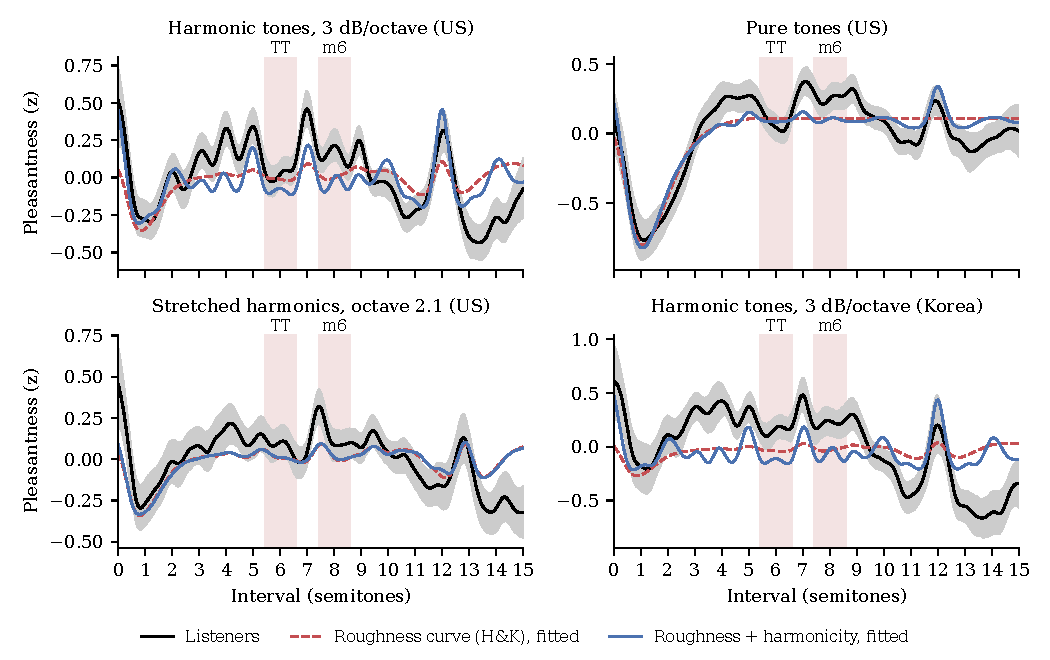
\includegraphics[width=\linewidth]{figures/fig_profiles.pdf}
\caption{聽者愉悅度剖面（黑線；灰帶為 95\% 自助法信賴區間），並附粗糙度曲線（\HK，紅色虛線）
與粗糙度加諧波度曲線（藍線）；兩者皆以陰影視窗（三全音 TT 與小六度 m6）以外的所有音程對聽者校準。
諧波音（左上）；純音（右上）；拉伸分音（左下）；韓國聽者，諧波音（右下）。
（圖中座標軸文字沿用原文，為英文。）}
\label{fig:profiles}
\end{figure}

\subsection{粗糙度}
\label{sec:roughness}
表~\ref{tab:gap} 列出每項實驗的差距。對滾降為 3\,dB/八度的諧波音，小六度的評分比三全音高
\gapObsHarm\SDu{} \gapObsHarmCI，而經校準的 \HK{} 粗糙度所留下的差距為 \gapHKHarm\SDu{} \gapHKHarmCI。
在六項頻譜為諧波的美國實驗上合併後，觀測差距為 \poolGapObsHarm\SDu{} \poolGapObsHarmCI，
經校準的 \HK{} 粗糙度所留下的差距為 \poolGapHKHarm\SDu{} \poolGapHKHarmCI，
亦即觀測差距的 \poolLeftHK\%（表~\ref{tab:pooled}）；Sethares 核則留下 \poolGapSethHarm。
在四度與五度之間，粗糙度曲線幾乎是平的，因此一旦校準，它對三全音與小六度預測出幾乎相同的愉悅度。
粗糙度能把三全音與低位分音重合的四度、五度區分開來，但在三全音與小六度處，
確實發生交互作用的近失（near-miss）分音對，對這些頻譜產生了相近的總量。
經校準的曲線確實部分重現了三全音低於四度與五度的凹陷（合併後留下的凹陷為 \poolDipHKHarm，
觀測值為 \poolDipObsHarm），這就是為什麼凹陷與差距講的是不同的故事。
對於純音，其分音在這些音程上不發生交互作用，粗糙度預測沒有差距，然而聽者卻產生了差距
（\gapObsPure\SDu{} \gapObsPureCI）。

\begin{table}[t]
\centering
\caption{差距（小六度減三全音）：觀測值，以及各模型以實驗本身校準後所留下的未解釋部分，
單位為聽者內 SD [95\% 受試者自助法信賴區間]。粗體：信賴區間排除零。
\citet{marjieh2024} 的複合模型是以這些資料擬合的。$N$：受試者人數。}
\label{tab:gap}
\footnotesize
\setlength{\tabcolsep}{4pt}
\resizebox{\linewidth}{!}{%
\begin{tabular}{lrcccc}
\toprule
& & & \multicolumn{3}{c}{校正後留下的未解釋部分} \\
\cmidrule(lr){4-6}
實驗 & $N$ & 觀測值 & 粗糙度 & 粗糙度 + 諧波度 & 複合模型 \\
\midrule
\tabinput{tables_zh/tab_mj_gap.tex}
\bottomrule
\end{tabular}}
\end{table}

\subsection{諧波度彌補了三全音自身的不足}
\label{sec:harmonicity}
加入諧波度（已發表的容忍度）後，合併差距為 \poolGapHKHHarm\SDu{} \poolGapHKHHarmCI，
即觀測差距的 \poolLeftHKH\%，且異質性很大（$I^2=\poolGapHKHHarmItwo\%$；表~\ref{tab:pooled}）。
主要估計目標，即容忍度 20 音分的曲線在留出情況下的差距，為 \primGap\SDu{} \primGapCI{}
（$\tau=\primTau$，$I^2=\primItwo\%$）。本文中有三個相近的數值，回答的是不同的問題：
\primGap{} 是主要估計目標（留出、容忍度 20 音分、隨機效應、Hartung--Knapp 區間）；
表~\ref{tab:pooled} 中的 \poolGapHKHHarm{} 是描述性校準，採用已發表的容忍度，且每項實驗各自擬合；
而第~\ref{sec:lodo}~節中的 \mbGapHKHtw{} 則是 20 音分曲線在六種頻譜上的留出差距，取普通平均。
主要估計目標是一個真實的差距，但對新的諧波頻譜而言，其預測區間 \primGapPI{} 包含零，
而逐一頻譜來看，範圍從 \primNothree{}（不含第三諧波的五個諧波）到 \primGuitar{}（吉他）。
合成頻譜留下的很少（諧波音 \primHarm，五個等振幅諧波 \primEqfive）；
重新合成的長笛、吉他與鋼琴留下的最多（\primFlute、\primGuitar{} 與 \primPiano）。
由於我們為這三種樂器所取得的頻譜是代用品，這個對比所反映的，
可能是模型看不到的頻譜細節，而不只是聽者的性質。

描述性的校準結果一致。不含粗糙度的諧波度留下較少的差距（\poolGapHHarm），
但對音程軸其餘部分的擬合較差：在排除視窗之外，它對五個等振幅諧波、不含第三諧波的五個諧波與長笛的剖面，
分別解釋 $R^2=\rfitHEqfive$、\rfitHNothree{} 與 \rfitHFlute{}，
而粗糙度加諧波度則為 \rfitHKHEqfive、\rfitHKHNothree{} 與 \rfitHKHFlute。
參數是以這些實驗擬合的 \citet{marjieh2024} 複合模型，留下 \poolGapCompHarm；
而採用 \texttt{incon} 的模板（而非 Marjieh 等人的模板）計算的諧波度則留下 \poolGapInconHarm。
凹陷對諧波度如何加權更為敏感：觀測值為 \poolDipObsHarm\SDu，經粗糙度與諧波度後為
\poolDipHKHHarm{} \poolDipHKHHarmCI，僅經諧波度後為 \poolDipHHarm，經複合模型後為 \poolDipCompHarm{}
（補充材料表~\ref{S-tab:dip}）。由於凹陷是把三全音與其緊鄰的音程比較，
而差距則是把它與位於五度另一側的音程比較，兩者不必一致，下一段會說明它們為何不一致。

\paragraph{差距的哪一端？}
差距是一個差值，$r(8)-r(6)$，因此它可以出自任一端。表~\ref{tab:ends} 將它拆開。
僅用粗糙度時，三全音偏離其預測 \rpfSixHK\SDu，小六度偏離 \rpfEightHK；
相對於小二度至大七度之間其他音程的平均殘差，三全音低了 \rpfTTOtherHK。
因此三全音的不足是相對的，在絕對意義上並不可靠地為負，
而在吉他、鋼琴與不含第三諧波的五個諧波上最為明顯。以容忍度 20 音分加入諧波度後，
三全音移至 \rpfSixTw，它與其他音程的差異移至 \rpfTTOtherTw，兩者皆無法與零區分，
而小六度維持在 \rpfEightTw。差距所剩下的，是小六度被評得高於曲線。
小六度在這方面並不特殊：它的殘差與小三度與大三度、四度、五度和大六度的平均並無差異
（\rpfMsixConsTw；表~\ref{tab:resprofile}）。這些殘差是相對於以音程軸其餘部分擬合的截距而言，
因此它們指出的是曲線形狀在哪裡有誤，而非絕對水準。純音亦然
（三全音 \rpfPureTwSix，小六度 \rpfPureTwEight；點估計）。

\begin{table}[t]
\centering
\caption{差距的哪一端。三全音處的留出殘差 $r(6)$ 與小六度處的留出殘差 $r(8)$（觀測值 $-$ 預測值），
分別在 \HK{} 粗糙度之下與推薦曲線（\HK{} + 諧波度，容忍度 20 音分）之下，
以及後者所留下的差距，單位為 SD [受試者自助法信賴區間]。合併列：六種諧波頻譜上的隨機效應，
Hartung--Knapp 信賴區間；其最後一格即為主要估計目標。粗體：信賴區間排除零。}
\label{tab:ends}
\footnotesize
\setlength{\tabcolsep}{3pt}
\resizebox{\linewidth}{!}{%
\begin{tabular}{lccccc}
\toprule
& \multicolumn{2}{c}{粗糙度（\HK）} & \multicolumn{2}{c}{\HK{} + 諧波度（20 音分）} & \\
\cmidrule(lr){2-3}\cmidrule(lr){4-5}
實驗 & $r(6)$ & $r(8)$ & $r(6)$ & $r(8)$ & 剩餘差距 \\
\midrule
\tabinput{tables_zh/tab_ends.tex}
\bottomrule
\end{tabular}}
\end{table}

\begin{table}[t]
\centering
\caption{隨機效應合併估計 [95\% Hartung--Knapp 信賴區間] 與對新實驗的 95\% 預測區間（PI），
單位為 SD，各模型以實驗本身校準。諧波：六項頻譜為諧波的美國實驗。八項：另加純音與邦囊。
$^{a}$以這些資料擬合。DerSimonian--Laird 區間：補充材料表~\ref{S-tab:suppdl}。}
\label{tab:pooled}
\footnotesize
\setlength{\tabcolsep}{3.5pt}
\resizebox{\linewidth}{!}{%
\begin{tabular}{lcccccc}
\toprule
& \multicolumn{2}{c}{差距，諧波（$k=\kHarm$）} & \multicolumn{2}{c}{差距，八項（$k=\kEight$）}
& \multicolumn{2}{c}{凹陷，諧波（$k=\kHarm$）} \\
\cmidrule(lr){2-3}\cmidrule(lr){4-5}\cmidrule(lr){6-7}
& 估計值 [CI] & PI & 估計值 [CI] & PI & 估計值 [CI] & PI \\
\midrule
\tabinput{tables_zh/tab_pooled.tex}
\bottomrule
\end{tabular}}
\end{table}

\begin{figure}[t]
\centering
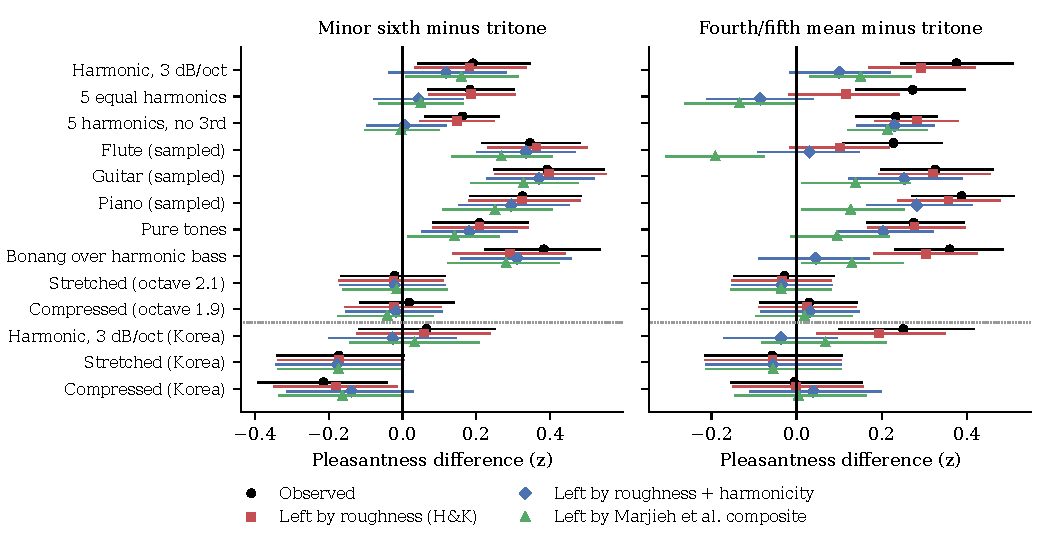
\includegraphics[width=\linewidth]{figures/fig_forest.pdf}
\caption{觀測差距與凹陷（黑），以及各模型所留下的未解釋部分：粗糙度（紅）、
粗糙度加諧波度（藍）與擬合後的 \citet{marjieh2024} 複合模型（綠），
逐實驗呈現，各模型以實驗本身校準，附 95\% 自助法信賴區間。
虛線以下：拉伸與壓縮頻譜以及韓國組。（圖中座標軸文字沿用原文，為英文。）}
\label{fig:forest}
\end{figure}

\paragraph{調音。}
以較窄的核（SD 為 0.1 個半音；探索性）定位時，聽者的小六度峰值位於 \ejLocMsix{} 音分，
介於十二平均律與 8/5（\jiCentsMsix{} 音分）之間，且與諧波度模型的峰值相差 \ejDiffMsix{} 音分；
在純律位置處所剩的差距也並沒有較小（差異 \ejGapJIaDiff），
因此這些資料無法判斷聽者是把小六度聽成平均律還是純律（無定論；補充材料第~\ref{S-sec:etji}~節）。

\subsection{在留出頻譜上更好的曲線}
\label{sec:lodo}
以橫跨各美國實驗擬合的一組權重（已發表的容忍度），並讓每項實驗由以其他實驗擬合的權重來預測
（表~\ref{tab:lodo}），留出的未解釋差距在 \lodoN{} 項實驗中有 \lodoPos{} 項為正，
其中 \lodoExcl{} 項的信賴區間排除零；對諧波頻譜，6 項中有 \lodoPosHarm{} 項為正，
\lodoExclHarm{} 項排除零。在未見頻譜上的殘差與描述性的殘差落在同一範圍，
因此它並非對每項實驗重新擬合的人為產物。

\paragraph{預先指定的篩選。}
在查看之前，我們先確定了一份候選第三因素清單，它們全都由刺激計算而得，
也不繫於任何特定音程，並確定了一項準則：對留出實驗的預測。候選項目為：
（1）諧波度模型中較寬的失準容忍度，即頻譜與模板的高斯寬度 $\sigma$，在每一摺內自 6.83、10、15 或 20 音分中選取；
（2）根音歧義（root ambiguity）\citep{terhardt1974,parncutt1988}，即虛擬音高剖面中第二高峰相對於最高峰的高度；
（3）時間週期性，即分音在 2--30\,ms 延遲上的最大正規化自相關 \citep{pressnitzer2001}，
精神上近於 \citet{stolzenburg2015} 與 \citet{masina2022}；以及（4）作為刻意設置的對照，
頻率比的諧波熵（harmonic entropy）\citep{erlich}，它忽略頻譜。
基準模型在每一摺內重新擬合。清單事先已經確定，但並未公開註冊。

只有容忍度有幫助（表~\ref{tab:screen}）。各摺所選的結果在每一摺都是 $\sigma=\scrChosenSigma$ 音分，
此二項曲線的平均留出 $R^2$ 為 \mbRtwoHKHtw，對照已發表容忍度的 \mbRtwoHKH{}（配對差 \mdRtwoTwVsHKH）、
修正粗糙度加諧波度的 \mbRtwoRev{}，以及 \citet{marjieh2024} 複合模型的 \mbRtwoComp{}
（配對差 \mdRtwoTwVsComp；對整個逐一留出程序做 \mbNboot{} 次受試者自助法）。
複合模型的內部權重是以這些實驗擬合的，因此這項比較對它有利。
一旦諧波度已在模型中，根音歧義（$R^2=\scrRtwoRA$）與週期性（$R^2=\scrRtwoPER$）並無增益，
對照項也沒有增益（$R^2=\scrRtwoHE$）。事後檢查（探索性）顯示，最佳值取決於平滑：
核為 0.1 個半音時，最佳容忍度為 \rbBestSigmaOne{} 音分，10、15 與 20 音分幾乎並列
（\rbRtwoOneTen、\rbRtwoOneFifteen、\rbRtwoOneTwenty），核為 0.3 個半音時則為 \rbBestSigmaThree。
比已發表值更寬的容忍度在每種寬度下都有幫助（$R^2$ 增益 \rbGainOne、\rbGainTwo{} 與 \rbGainThree），
但 20 音分只是一個有代表性的數值，並非估計值。篩選之後才檢視的各列見補充材料表~\ref{S-tab:screenexpl}。

在進行平滑檢查之前，我們已設定一項準則：在較窄與較寬的核下，最佳容忍度都應落在 15--25 音分；
在 0.3 個半音時達成，在 0.1 個半音時則未達成，那時有些摺選了 10 音分。
每個二音組的低音是從 G3 到 F4 取樣，而模型把它放在 C4；對該範圍內的 \HK{} 粗糙度取平均，
會使推薦曲線的留出 $R^2$ 改變 \rbdRtwoRegVsHKHtw{}，而諧波度不受移調影響。
音域確實會改變純音二音組的整體喜好度 \citep{kaklamani2025}，
但一項實驗中所有音程共有的位移會被其截距吸收。

容忍度改善了整條曲線，卻幾乎沒有動到差距：六項諧波實驗中的留出差距為 \mbGapHKHtw\SDu，
已發表容忍度下則為 \mbGapHKH，而沒有任何候選項移除了它。容忍度、歧義與週期性合在一起達到
$R^2=\scrRtwoAll$，並留下 \scrGapAll 的差距。殘差集中於純音（\scrGapTwPure）
與重新合成的長笛、吉他與鋼琴（\scrGapTwFlute、\scrGapTwGuitar{} 與 \scrGapTwPiano）。
對照項在第二點上也如預期失敗：由於它只取決於頻率比，它必然也把拉伸音的懲罰放在 600 音分
（在擬合曲線中為 \scrHEpredDipSix\SDu），而聽者在該處並無此現象（第~\ref{sec:tests}~節）。
在連續取樣的二音組中，較寬的容忍度僅意味著聽者的協和峰比模型的更寬；
它並不是關於十二平均律本身的證據（第~\ref{sec:chords}~節）。

\begin{table}[t]
\centering
\caption{逐一留出實驗的預測（已發表的容忍度）。$b_R$、$b_H$：以其他美國實驗擬合的粗糙度與諧波度權重。
留出的未解釋差距與凹陷 [95\% CI]，單位為 SD。粗體：信賴區間排除零。}
\label{tab:lodo}
\footnotesize
\setlength{\tabcolsep}{4pt}
\resizebox{\linewidth}{!}{%
\begin{tabular}{lrrccc}
\toprule
留出的實驗 & $b_R$ & $b_H$ & 差距，僅粗糙度 & 差距，兩種機制 & 凹陷，兩種機制 \\
\midrule
\tabinput{tables_zh/tab_lodo.tex}
\bottomrule
\end{tabular}}
\end{table}

\begin{table}[t]
\centering
\caption{預先指定的樣本外篩選（逐一留出一項美國實驗；點估計）。
$R^2$：對整個剖面擬合的各留出實驗平均（10 項美國實驗；六項諧波實驗）。
差距、凹陷：所留下的未解釋部分，六項諧波實驗的平均。TT $-$ 其他：三全音的殘差凹陷減去其他 13 個音程的平均
（八項未拉伸的實驗）。拉伸：拉伸分音在 6.00 個半音處以及在拉伸音階的三全音位置 6.42 處的殘差凹陷。
單位為 SD。事後各列：補充材料表~\ref{S-tab:screenexpl}。}
\label{tab:screen}
\footnotesize
\setlength{\tabcolsep}{3pt}
\resizebox{\linewidth}{!}{%
\begin{tabular}{lccccccc}
\toprule
& \multicolumn{2}{c}{留出 $R^2$} & & & & \multicolumn{2}{c}{拉伸，剩餘凹陷} \\
\cmidrule(lr){2-3}\cmidrule(lr){7-8}
模型 & 10 項美國 & 6 項諧波 & 剩餘差距 & 剩餘凹陷 & TT $-$ 其他 & 於 6.00 & 於 6.42 \\
\midrule
\tabinput{tables_zh/tab_screen.tex}
\bottomrule
\end{tabular}}
\end{table}

\begin{figure}[t]
\centering
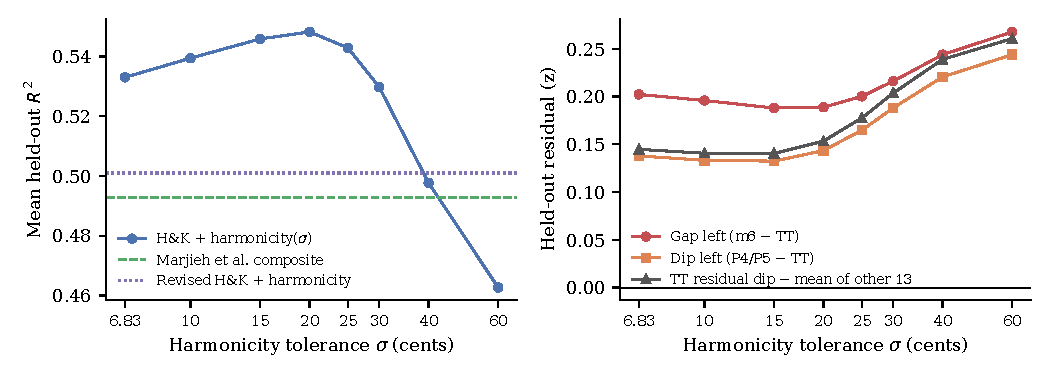
\includegraphics[width=\linewidth]{figures/fig_sigma.pdf}
\caption{諧波度容忍度。左：高斯寬度 $\sigma$ 變動時，粗糙度加諧波度的平均留出 $R^2$（已發表值為 6.83 音分），
對照修正粗糙度加諧波度與 \citet{marjieh2024} 複合模型。右：留出的諧波實驗上所剩的三全音殘差。
超過 20 音分的數值是在篩選之後才檢視的。（圖中座標軸文字沿用原文，為英文。）}
\label{fig:sigma}
\end{figure}

\subsection{三全音特殊嗎？}
\label{sec:special}
表~\ref{tab:resprofile} 列出每個整數音程上的留出殘差，在六種諧波頻譜上以隨機效應合併。
僅用粗糙度時，小二度至大七度之間最為負向的殘差是大二度（\rpfMajSecHK）與三全音（\rpfSixHK）。
以容忍度 20 音分加入諧波度後，協和音程——三度、四度、五度與六度——位於曲線之上
（小三度 \rpfMinThirdTw、四度 \rpfFourthTw、五度 \rpfFifthTw、大六度 \rpfMajSixthTw），
而二度、三全音與小七度則靠近曲線（三全音 \rpfSixTw、大二度 \rpfMajSecTw、小七度 \rpfMinSevTw），
大七度位於曲線之上（\rpfMajSevTw）。因此三全音只是曲線預測得大致正確的幾個音程之一，
並非一個可偵測地被評得低於曲線的音程。若改以「低於其兩側鄰近音程的凹陷」來衡量，
經諧波度後（已發表的容忍度）三全音的凹陷與一般音程的平均相差 \ttoHKHHarm{} \ttoHKHHarmCI{}（六種諧波頻譜），
該區間包含零，但加入純音與邦囊後則為 \ttoHKHEight{} \ttoHKHEightCI；
在 \citet{marjieh2024} 的複合模型下，八種頻譜的數字為 \ttoCompEight{} \ttoCompEightCI。
這些區間針對已發表的容忍度；對 20 音分的曲線則只有點估計（表~\ref{tab:screen}）。
我們報告八種頻譜的數字，而不將它剔除。由於三全音自身的殘差並未低於平均，
該超額反映的是兩側的四度與五度被評得高於曲線，而不是三全音有所不足。
各音程的凹陷見補充材料圖~\ref{S-fig:null}。

\begin{table}[t]
\centering
\caption{每個整數音程上的留出殘差（觀測值 $-$ 預測值），六種諧波美國頻譜上的隨機效應，單位為 SD。
$^*$Hartung--Knapp 信賴區間排除零。Size：音程大小的線性項（第~\ref{sec:ceiling}~節）。
（欄標中的 m2、M2、m3、M3、P4、TT、P5、m6、M6、m7、M7、P8、m9、M9 依序為小二度、大二度、小三度、大三度、
純四度、三全音、純五度、小六度、大六度、小七度、大七度、八度、小九度、大九度。）}
\label{tab:resprofile}
\scriptsize
\setlength{\tabcolsep}{2pt}
\resizebox{\linewidth}{!}{%
\begin{tabular}{lcccccccccccccc}
\toprule
模型 & m2 & M2 & m3 & M3 & P4 & TT & P5 & m6 & M6 & m7 & M7 & P8 & m9 & M9 \\
\midrule
\tabinput{tables_zh/tab_resprofile.tex}
\bottomrule
\end{tabular}}
\end{table}

\paragraph{對準音程的加成與一個階躍（探索性）。}
我們在看過殘差剖面之後又發現了兩種型態。兩者都是對「容忍度 20 音分並加入音程大小線性項」之曲線的留出殘差計算的
（該線性項吸收了第~\ref{sec:ceiling}~節的平滑趨勢）。第一種是局部加成：
十二平均律音程 $c$ 處的殘差，減去其兩側四分音處殘差的平均，
$b(c)=r(c)-[r(c-0.5)+r(c+0.5)]/2$。在諧波頻譜上合併後，小二度至大七度之間、三全音以外的各音程，
平均加成為 \decTwoBonusOther\SDu，三全音為 \decTwoBonusTT；各音程的加成從
\decTwoBMinSev{}（小七度）與 \decTwoBMajSec{}（大二度）到 \decTwoBMajThird{}（大三度）不等。
三全音相對於其他音程的不足，\decTwoOtherMinusTT，包含零。資料確實能區分的、而我們也是在看過剖面後才注意到的，
是大二度與小七度所獲得的加成小於其他八個音程（\decTwoMMvsRest，$I^2$ 接近零）；
三全音與它們並無差異（\decTwoTTvsMM）。更粗糙的小二度與大七度則獲得完整的加成，
而我們不知道是什麼把這三個加成較小的音程區分出來。

這個加成屬於諧波音。以同樣方式在含尖銳度項的曲線（第~\ref{sec:ceiling}~節）上計算，
諧波頻譜為 \gbSharpHarmOther{}，但純音為 \gbSharpPure{}，邦囊為 \gbSharpBonang，
而在拉伸與壓縮音的任一音階上，它都無法與零區分（第~\ref{sec:tests}~節）。
它在更換諧波度模型後依然存在：擬合兩個寬度不同的諧波度項保留了其大部分，
採用已發表的容忍度與 Marjieh 等人的修正粗糙度（它使略微失準音程的慢拍變得悅耳）亦然。
在 0.2 個半音的平滑寬度下，加成無法分辨十二平均律與純律，因此我們把它解讀為對熟悉音程「鄰近範圍」的加成，
而非對其確切調音的加成。\citet{marjieh2024} 指出音色效應的細節仍有待其模型解釋；
我們尚不知有人量化過這項加成。

第二種型態是一個階躍。把 $r(c)$ 寫成 $b(c)+q(c)$，其中 $q(c)$ 為兩個相鄰四分音處殘差的平均，
差距便拆成加成部分 $b(8)-b(6)$（\decTwoBonusPart）與基線部分 $q(8)-q(6)$（\decTwoBasePart）；
在扣除線性趨勢後，以指標變數表示，基線在 7 至 8 個半音之間上升 \decTwoStep{}（$I^2=\decTwoStepItwo\%$）。
以頻譜上的普通平均而言，兩個部分都排除零（\decTwoBonusPartFixed{} 與 \decTwoBasePartFixed），
但在隨機效應下只有基線部分排除零，且這種拆分在各頻譜之間並不穩定（表~\ref{tab:decomp}）。
合成諧波音（\decTwoStepHarm）與長笛（\decTwoStepFlute）沒有階躍，吉他（\decTwoStepGuitar）與鋼琴（\decTwoStepPiano）則很大。
吉他與鋼琴的頻譜是代用品，各只有一個被分析的音，因此階躍可能來自頻譜模型而非聽者。
階躍對核寬、排除視窗與分箱都穩健（補充材料表~\ref{S-tab:step}）；它不穩健的是頻譜。
因此我們不把差距拆成固定份額的階躍與加成。

\begin{table}[t]
\centering
\caption{留出差距的分解（探索性；\HK{} + 20 音分諧波度 + 音程大小），逐一諧波頻譜 [受試者自助法信賴區間]，
以及以隨機效應合併 [Hartung--Knapp 信賴區間]。加成部分 $b(8)-b(6)$；基線部分 $q(8)-q(6)$；
階躍：扣除線性趨勢後，基線在 7 與 8 個半音之間的上升；其他 $-$ TT：其他音程的平均加成減去三全音的加成。
粗體：信賴區間排除零。吉他與鋼琴使用代用頻譜。}
\label{tab:decomp}
\footnotesize
\setlength{\tabcolsep}{3pt}
\resizebox{\linewidth}{!}{%
\begin{tabular}{lccccc}
\toprule
頻譜 & 剩餘差距 & 加成部分 & 基線部分 & 階躍 & 其他 $-$ TT 加成 \\
\midrule
\tabinput{tables_zh/tab_decomp_spectra.tex}
\bottomrule
\end{tabular}}
\end{table}

\subsection{殘差取決於什麼}
\label{sec:tests}

\paragraph{頻譜。}
當分音被拉伸或壓縮時，600 音分處的未解釋差距約為零（美國，經粗糙度與諧波度後：
\gapHKHStr{} 與 \gapHKHComp\SDu），觀測凹陷也是如此（\dipObsStr{} 與 \dipObsComp），
儘管剖面並不平坦（剖面 SD 為 \profSDStr{} 與 \profSDComp，諧波音則為 \profSDHarm）。
若懲罰是依附於實體的 600 音分音程，它在拉伸後應該依然存在，因為基頻仍然相距 600 音分。
當分音拉伸至八度比 $r$ 時，與頻譜相符的音階，其三全音位於 $6\log_2 r$ 個半音處：
拉伸音為 \sscPosStr{}，壓縮音為 \sscPosComp。在那個位置，拉伸音出現觀測凹陷 \sscObsDipStr\SDu，
而在 6 處原本沒有（配對差 \sscObsDipStrDiff）。留出的 \HK{} 粗糙度在該位置預測出 \mbStrPredHK{} 的凹陷，
並留下 \mbStrSscHK{} \mbStrSscHKCI；依附於頻率比的對照項則必然把它的懲罰放在 600 音分處。
對壓縮音而言，\sscPosComp{} 處的凹陷並不顯著（\sscObsDipComp），
而韓國聽者在兩個位置都沒有明確的凹陷，因此這個位移僅建立在一種頻譜與一個受試族群上。

第~\ref{sec:special}~節的準音加成並不跟隨拉伸後的音階。在拉伸音階自身的音程上，平均加成為 \sbOwnStr{}
（壓縮為 \sbOwnComp），而諧波音為 \sbOwnHarm，這些資料能以 80\% 檢定力偵測的最小效應為 \sbMdeStr\SDu{}
（補充材料表~\ref{S-tab:strbonus}；探索性）。韓國聽者呈現相同型態（諧波 \sbOwnHarmKr，拉伸 \sbOwnStrKr）。
凹陷隨分音移動；加成則留在諧波音上。

已發表的諧波度模型無法跟隨位移後的凹陷，因為它的模板是一個諧波序列。
把模板換成上方音自身的分音（這是對「諧波模板是從所聽聲音中習得的」這項提議 \citep{shamma2000} 的一種解讀），
可以重現拉伸音階上的凹陷，但對諧波音的預測較差，因此它並不是一條更好的通用曲線
（探索性；補充材料第~\ref{S-sec:timbrerel}~節）。

\paragraph{針對性檢定。}
四項事先確定的對比，探查經粗糙度與諧波度後的殘差（表~\ref{tab:holm}）；
對它們做 Holm 校正是在此版本中加入的。韓國減美國聽者，相同的諧波刺激：\holmEstCulture{}（$p=\holmPCulture$）。
音樂人（受訓超過兩年）減非音樂人，在八項未拉伸的美國實驗上合併：\holmEstMus{}（$p=\holmPMus$）。
不含第三諧波的五個諧波減含第三諧波者，凹陷的觀測變化減去粗糙度所預測的變化（\nthreeHKDip）：
\holmEstThird{}（$p=\holmPThird$）。滾降由 2 變到 12\,dB/八度時差距的變化，觀測值減去粗糙度預測值：
\holmEstRoll{}（$p=\holmPRoll$）。經 Holm 校正後，四項中有 \holmNsurvive{} 項仍顯著（校正後 $p$ 從 \holmPadjThird{} 到 \holmPadjRoll）。

逐項來看，這些對比說明如下。音樂人顯示出較大的觀測差距與凹陷（\musPoolGap{} 與 \musPoolDip；表~\ref{tab:tests}），
其中一部分源自諧波度——音樂人對它更敏感 \citep{mcdermott2010}。經粗糙度與諧波度後，
音樂人的差距為 \grpMusGapHKH{}，非音樂人為 \grpNonGapHKH，兩者的差異皆包含零
（差距 \musPoolGapHKH，凹陷 \musPoolDipHKH），因此這些資料並未確立受過訓練的聽者有較大的殘差；
殘差在非音樂人身上同樣存在。對拉伸與壓縮分音，兩組並無差異（差距之差 \musPoolStrGap；兩項實驗的固定效應合併）。
韓國聽者對諧波音顯示較小的差距，但他們對拉伸與壓縮分音也以相同方向與美國聽者不同
（\cohObsGapStr{} 與 \cohObsGapComp），而美國聽者在那裡沒有差距，因此這個差異並非協和性所特有。
移除第三諧波使觀測凹陷的改變小於粗糙度所預測的（觀測變化 \nthreeObsDip），
與 \citet{marjieh2024} 一致，他們發現第三諧波是透過諧波度而重要；校正之後，這只能說是具有提示性。
在滾降實驗中，差距在 2、7 與 12\,dB/八度分別為 \rollTwoGap、\rollSevenGap{} 與 \rollTwelveGap\SDu，
而經校準的粗糙度預測為 \rollTwoHKpred、\rollSevenHKpred{} 與 \rollTwelveHKpred：
差距並未隨高位分音（以及隨之而來的粗糙度）的淡出而縮小（補充材料表~\ref{S-tab:rolloff}）。

\paragraph{文化與平滑趨勢。}
模型對韓國剖面的擬合不佳（粗糙度加諧波度，諧波音的樣本內 $R^2=\profRfitHarmKr$），
儘管它們的上限很高（\krCeilMin--\krCeilMax）。以美國聽者的權重預測時，推薦曲線的表現
比各實驗自身的平均更差（平均留出 $R^2$ 為 \krHoTw）；加入音程大小的線性項使它升至 \krHoSize，
再加尖銳度代用量則升至 \krHoSharp（補充材料表~\ref{S-tab:korean}；探索性）。
因此在這些資料中，區分兩組受試者的，主要是愉悅度隨音程大小下降得更陡，而不是協和性排序不同。
其原因尚無定論：尖銳度隨音程大小上升，是一個候選；在線上研究中，播放設備也是一個候選，因為兩組之間可能有所不同。

\begin{table}[t]
\centering
\caption{四項預先指定的針對性檢定，針對經粗糙度與諧波度（已發表的容忍度）後的殘差。
SE 來自受試者自助法（音樂訓練：八項實驗上的隨機效應，Hartung--Knapp SE，7 自由度的 $t$）。
$p$：雙尾；Holm：對四項校正後。}
\label{tab:holm}
\footnotesize
\begin{tabular}{p{0.56\linewidth}rrrr}
\toprule
對比 & 估計值 & SE & $p$ & Holm $p$ \\
\midrule
\tabinput{tables_zh/tab_holm.tex}
\bottomrule
\end{tabular}
\end{table}

\begin{table}[t]
\centering
\caption{組間差異 [95\% 自助法信賴區間]，單位為 SD。音樂訓練各列給出音樂人／非音樂人的人數。
粗體：信賴區間排除零（未校正）。}
\label{tab:tests}
\footnotesize
\setlength{\tabcolsep}{4pt}
\resizebox{\linewidth}{!}{%
\begin{tabular}{lcccc}
\toprule
& 觀測差距 & 粗糙度 + 諧波度後的差距 & 觀測凹陷 & 粗糙度 + 諧波度後的凹陷 \\
\midrule
\tabinput{tables_zh/tab_tests.tex}
\bottomrule
\end{tabular}}
\end{table}

\subsection{和弦}
\label{sec:chords}
以十二平均律計分——如 \texttt{incon} 以及先前的分析（包括作者的一項分析）——
十二個 Bowling 二音組呈現出密集資料的型態（表~\ref{tab:bowling}）：
粗糙度重現了三全音與小六度之差的 \bshareHKET\%，粗糙度加諧波度則重現 \bshareHKHET\%。
在和弦中，僅控制和弦大小時，每個三全音使評分下降 \bpenSizeET{} 個評分單位；
經粗糙度與諧波度後為 \bpenHKHET{} \bpenHKHETCI。但這些和弦是以純律演奏的。
在實際呈現的調音下，諧波度對小六度（8/5）的評價較高
（\harmJIMsix{}，十二平均律下為 \harmETMsix），而三全音（7/5）幾乎沒有變化
（\harmJITT{}，對照 \harmETTT）。依實際呈現的調音計分，粗糙度加諧波度重現了二音組差異的 \bshareHKHJI\%，
和弦層級的三全音懲罰降為 \bpenHKHJI{} \bpenHKHJICI。由於只有十二個二音組，這個比例是容易過度擬合的統計量；
以含有三全音的 \bNTT{} 個和弦估計的和弦層級懲罰，才是比較穩固的結果。

Johnson-Laird 的和弦是十二平均律的，在那裡仍留有懲罰：經粗糙度與諧波度後，每個三全音 \jpenHKH{}
\jpenHKHCI{} 個評分單位（評分 SD 為 \jRatingSD），加入熟悉度後為 \jpenHKHF{} \jpenHKHFCI。
這些和弦排列寬廣，且由不同的族群評分，因此兩組資料不能直接比較。
20 音分的容忍度把 Johnson-Laird 的懲罰降至 \csJLTwenty{} \csJLTwentyCI{}（配對差 \csJLDiff），
已無法與零區分，但對純律的 Bowling 和弦擬合較差（$R^2$ 由 \csBJISevenRtwo{} 降至 \csBJITwentyRtwo），
因此適合聽者的容忍度取決於他們所聽到的調音。重新計分 Bowling 和弦也改變了諧波度相對於干涉與熟悉度的獨有變異量：
在控制和弦大小時，它從 \dRBSizeH{} 升至 \dRBjiSizeH，與另外兩者相當，完整模型的 $R^2$ 從 \RfullBSize{} 升至 \RfullBjiSize。
若不控制和弦大小，熟悉度看來占主導，一如作者先前的分析所報告的（補充材料表~\ref{S-tab:chorddecomp}）。

\begin{table}[t]
\centering
\caption{\citet{bowling2018}：各擬合模型所重現的三全音—小六度二音組差異的比例（\%）（12 個二音組），
以及和弦中的三全音懲罰（每個三全音的評分單位，控制和弦大小 [95\% CI]；$n=298$），
模型分別以十二平均律（ET）或實際呈現的純律（JI）音高計分。}
\label{tab:bowling}
\footnotesize
\setlength{\tabcolsep}{4pt}
\begin{tabular}{lcccc}
\toprule
& \multicolumn{2}{c}{二音組比例（\%）} & \multicolumn{2}{c}{和弦三全音懲罰} \\
\cmidrule(lr){2-3}\cmidrule(lr){4-5}
模型 & ET & JI & ET & JI \\
\midrule
\tabinput{tables_zh/tab_bowling_ji.tex}
\bottomrule
\end{tabular}
\end{table}

\subsection{曲線整體遺漏了多少}
\label{sec:ceiling}
折半（split-half）上限的範圍從 \ceilMin{} 到 \ceilMax{}（美國平均 \ceilUS）。在留出情況下，
推薦曲線捕捉了美國實驗中 \shBaseFrac\% 的可解釋變異，\citet{marjieh2024} 的複合模型則為 \shCompFrac\%。
不足之處並不在三全音。對單一實驗擬合時，殘差有共同的寬廣形狀：
音域中段的音程被評得高於曲線，而寬音程——尤其是超過八度者——則低於曲線。
加入音程大小的線性項便可消除其中大部分（諧波音的樣本內 $R^2$ 從 \insBaseHarmThree{} 升至 \insXHarmThree，
韓國平均則從 \insBaseKR{} 升至 \insXKR）。其斜率取決於頻譜：諧波音為每八度音程 \slopeHarmThree\SDu，
純音為 \slopePure，但五個等振幅諧波為 \slopeEqFive，長笛為 \slopeFlute；韓國聽者則為 \slopeKrMax{} 至 \slopeKrMin。
在此，音程大小與上方音的音高以及與尖銳度——頻譜偏向高頻的程度 \citep{zwicker2007}——相混淆。
在協和模型縮窄為粗糙度與諧波度之前，尖銳度曾是心理聲學中感官愉悅度的一個成分 \citep{aures1985}；
它會降低高音域和弦的協和性 \citep{eerola2022register}，而對純音二音組，偏好會隨平均頻率上升而下降
\citep{kaklamani2025}。

作為一項探索性比較（在看過殘差之後才選定），我們加入了一個平滑項，其權重由所有實驗共用。
美國留出 $R^2$ 從 \shBaseRtwoUS{} 升至：加音程大小時為 \shXRtwoUS，
加由合成參數計算的尖銳度代用量時為 \shSharpRtwoUS{}（配對差 \shdRtwoUSVsBase），
亦即可解釋變異的比例從 \shBaseFrac\% 升至 \shSharpFrac\%；相較之下，放寬容忍度只增加了 \shTolGain。
尖銳度相對於音程大小的優勢，是可能由挑選所造成的那一部分。這項增益並不取決於粗糙度模型：
採用 Marjieh 等人的修正粗糙度時，美國 $R^2$ 從 \shRevRtwoUS{} 升至 \shRevSharpRtwoUS。
它集中於合成頻譜（諧波音 \shBaseRtwoHarmThree{} 升至 \shSharpRtwoHarmThree，拉伸 \shBaseRtwoStr{} 升至 \shSharpRtwoStr），
並有兩種頻譜不符合它：五個等振幅諧波的趨勢不存在，儘管尖銳度隨音程上升；
而長笛的評分隨音程大小上升，在此反而變差（\shBaseRtwoFlute{} 降至 \shSharpRtwoFlute）。
滾降實驗在同一批受試者的各次試驗中改變頻譜斜率，提供了聽者內部的一項檢驗，
雖然我們是在選定尖銳度之前就看過它。在每個滾降下分別擬合時，
音程大小上的斜率從 1\,dB/八度的 \roSlopeOne{} 趨平到 13 時的 \roSlopeThirteen，一如尖銳度所預測、
而單靠音程大小無法預測的那樣，但代用量所隱含的斜率只涵蓋該趨平幅度的 \roImpShare\%。
最後，對於 \citet{marjieh2024} 尚未被分析的一組評分——\ctNPart{} 位受試者評定的 \ctNChords{} 個五個等振幅諧波的三和弦——
我們在讀資料之前寫下三項預測：尖銳度權重為負、逐一留出和弦的 $R^2$ 更好、
凍結權重的曲線與和弦平均的相關更佳。三項都沒有通過（權重 \ctBS；$R^2$ 之差 \ctLooDiff；相關之差 \ctRDiff；
補充材料第~\ref{S-sec:sharpness}~節），不過三和弦留給第三項的空間很小。
因此我們把平滑趨勢視為已確立，把尖銳度視為候選解釋，並且不把它加進推薦曲線。

\begin{figure}[t]
\centering
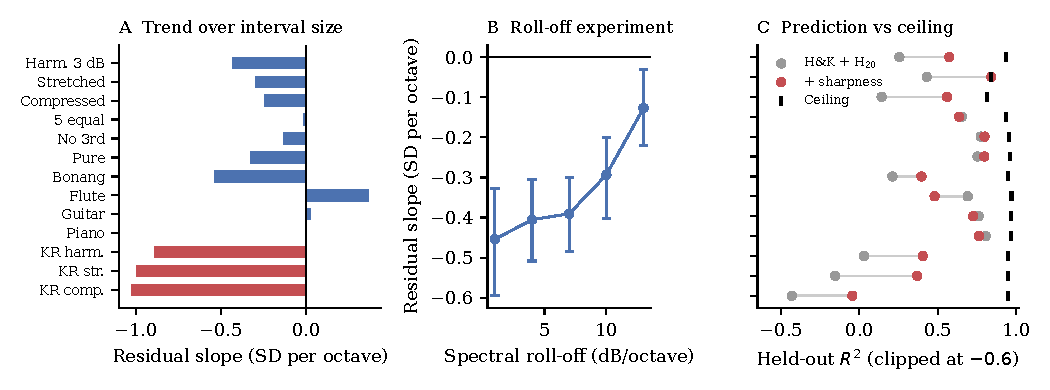
\includegraphics[width=\linewidth]{figures/fig_sharp.pdf}
\caption{平滑趨勢（探索性）。（A）\HK{} 粗糙度加諧波度（容忍度 20 音分）之殘差在音程大小上的斜率，
各實驗單獨擬合（每八度音程的 SD）。（B）滾降實驗中，各頻譜滾降下相同的斜率（受試者自助法 95\% CI）。
（C）各實驗在不含與含尖銳度項時的留出 $R^2$，對照折半上限（韓國實驗以所有美國實驗的權重預測）。
（圖中座標軸文字沿用原文，為英文。）}
\label{fig:sharp}
\end{figure}

% =====================================================================
\section{討論}

\subsection{什麼彌補了差距，以及推薦曲線}
\label{sec:curve}
對諧波音與美國聽者而言，小六度的評分比三全音高 \poolGapObsHarm{} 個聽者內 SD，
而以音程軸其餘部分校準的粗糙度曲線對此一分也預測不出：粗糙度在四度與五度之間幾乎是平的。
流行的診斷——不協和曲線過度簡化——在一個精確的意義上是正確的。所缺少的是諧波度。
三全音的分音與任何單一諧波序列都不太吻合，而小六度的分音則近似於那個以兩個基頻分別為第 5 與第 8 諧波的序列。
曲線中有了諧波度之後，三全音自身的不足便不再可偵測，而根音歧義、週期性與諧波熵都沒有增益：
分音無法契合任何單一序列的音程，正是其虛擬音高含糊的那個音程。

我們推薦的曲線為
$P(x)=\alpha_e+b_R\,R_{\mathrm{HK}}(x)+b_H\,H_{20}(x)$，其中 $R_{\mathrm{HK}}$ 為二音組合成頻譜的
Hutchinson--Knopoff 粗糙度，$H_{20}$ 為容忍度 20 音分的 Harrison 與 Pearce 諧波度
（11 諧波模板，權重 $1/i$，頻譜與模板採相同的高斯寬度，低音在 C4），兩者皆以 0.2 個半音的核平滑，
並且 20 音分曲線的合併權重為 $b_R=\scrBetaR$ 與 $b_H=\scrBetaH$
（每單位原始模型輸出；$\alpha_e$ 為實驗截距）。它沒有任何針對特定音程的項。
它對留出的美國實驗的預測優於我們所測試的已發表組合，但僅略優於採用已發表容忍度的同一曲線；
對純律的音，則已發表的容忍度擬合較佳。曲線的家族及其成分都並不新穎
\citep{parncutt2019,harrison2020,marjieh2024,masina2022}；
新的是它對三全音的預測，是在未用於擬合的實驗上、對照事先確定的候選項、並在一種會移動音程的頻譜上檢驗過的。

使用者須注意三點。第一，其權重適用於此處所測試的那類新頻譜；在實驗本身上，權重是在不含被預測實驗的情況下重新擬合的，
而截距使曲線只是關於剖面形狀的陳述，而非其水準。第二，容忍度既是一項心理聲學參數，也是一項平滑選擇，
因為它與同時平滑評分與模型輸出的核相互作用；在更精細的解析度下，20 音分的曲線會把聽者所顯示的小六度峰值平滑掉
（補充材料第~\ref{S-sec:etji}~節）。第三，該曲線是為十二平均律的音而設；
以純律呈現的和弦應依實際呈現計分，並採用已發表的容忍度。對音程大小加入一個平滑項，
會比我們在三全音處測試過的任何東西都更能改進它，但在其成因查明之前，我們把它排除在外。

\subsection{剩下什麼，以及如何解讀}
\label{sec:discussion-remains}
二音組中所剩的，是主要估計目標 \primGap\SDu{} \primGapCI，對描述性校準而言，
約為七點量表上的 \poolGapHKHHarmRaw{} 點。它在三方面並非常數。
它在不同頻譜之間的變動超出抽樣誤差所能容許的範圍（預測區間 \primGapPI），
最大值出現在所取樣樂器的代用頻譜上。當分音被拉伸或壓縮時，它在 600 音分處不存在。
而且它並非可偵測地屬於三全音：經諧波度後，三全音的殘差與零沒有差異，
而小六度位於曲線之上，其他協和音程亦然。探索性分解並未改變這一點。
它的階躍由兩種代用頻譜所承載，而一旦把頻譜視為隨機樣本，三全音降低的準音加成也無法使它與其他音程區分；
那個明確的對比——大二度與小七度的加成較小——是在看過剖面後才發現的。
我們不會在不協和模型中加入三全音懲罰。我們會加入諧波度，並去尋找：
是什麼使諧波音的協和音程比任何現有曲線所預測的更悅耳。

\paragraph{純音。}
純音看似會得出相反的結論：它們沒有可對齊的上方分音，卻留下最大的差距之一。殘差剖面解開了這個疑點。
對純音而言，三全音的預測大致正確（\rpfPureTwSix），差距來自小六度（\rpfPureTwEight），
因此純音一開始就沒有提供 600 音分處有懲罰的證據。由於它們的分音就是基頻，
純音無法區分頻譜的解釋與基於頻率比的解釋；只有分音偏離諧波序列的頻譜才能做到。

\paragraph{拉伸音與所聽到的八度。}
當分音被拉伸時，凹陷離開 600 音分，出現在拉伸音階的三全音處。作者先前的一項分析把這解讀為
與「相對於聽者實際聽到的八度所界定的習得類別」相容。這個解讀所預測的不只凹陷：
一個以所聽八度為中心重新定位的類別，也應把準音加成帶到拉伸音階的各音程上。它沒有
（\sbOwnStr，可偵測的效應為 \sbMdeStr，諧波音為 \sbOwnHarm）。凹陷跟隨分音而加成不然，
這有利於凹陷的頻譜解釋（兩個音的分音是否對齊），而不利於重新定位的習得類別。
這與「非諧波的鐘聲音色的協和判斷是跟隨其分音而非名義音程」的發現相符 \citep{harrison2024carillon}。
它僅建立在一種拉伸頻譜上；壓縮音在其自身的三全音處並未顯示明確的凹陷。

\paragraph{小六度殘差的兩種解讀。}
第一種是諧波度模型不完整。調音分析並未指認出缺陷所在：聽者的小六度峰值位於十二平均律與純律之間，
而在純律位置處差距也沒有較小。一個在其他某個細節上有誤的諧波度模型，必須解釋為什麼殘差在不同頻譜之間有變動、
為什麼其他協和音程也有、為什麼它在純律的 Bowling 和弦中消失，
以及為什麼在十二平均律的 Johnson-Laird 和弦中仍有懲罰。第二種解讀是習得的：
對調性音樂中協和音程的熟悉，這些音程多半是在諧波聲音中聽到的 \citep{lahdelma2022,mcdermott2016}。
準音加成符合這個解讀，因為它出現在諧波音上，而在拉伸與壓縮音的任一音階上都沒有。
但針對性檢定在經多重比較校正後，並不支持其通常的推論：無論是訓練 \citep[參見][]{mcdermott2010,popescu2019}
還是文化，都沒有可偵測地改變殘差。這兩種解讀正是當前爭論的雙方：
一方是把諧波度視為知覺機制的心理聲學解釋 \citep{harrison2020,marjieh2024}，
另一方是認為諧波度部分地代表了暴露經驗的看法 \citep{lahdelma2022,milne2023}。
我們的資料把殘差定位在諧波音的協和音程上；它們無法判斷哪一種解讀是對的。

和弦使對比更鮮明，卻沒有解決它。純律的 Bowling 和弦在經粗糙度與諧波度後沒有留下三全音懲罰，
而十二平均律的 Johnson-Laird 和弦留下了，20 音分的容忍度把它降到一個區間包含零的數值
（\csJLTwenty{} \csJLTwentyCI）。這正是一個低估十二平均律協和音程的不完整諧波度模型會產生的結果，
也正是對熟悉的十二平均律音程的習得偏好會產生的結果。這兩組和弦除了調音，
在排列與族群上也不同，而且在和弦中，三全音懲罰是從三全音的個數估計的，
因此和弦也沒有顯示三全音是特殊的；它們顯示的是，調音必須依實際呈現計分。

\paragraph{什麼能夠裁決。}
三項實驗可以區分這兩種解讀。以第二個拉伸係數與第二個受試族群重複拉伸頻譜的結果，
將檢驗凹陷是否普遍跟隨分音；以比區分兩種調音的 14 音分更精細的解析度，
密集取樣小六度與大三度區域，並在每種頻譜上有足夠的聽者，
將能把峰值定位得夠準，以判定諧波度模型是否把它們放錯了位置。
比較對十二平均律諧波音樂接觸很少的聽者，讓他們評定同樣的密集二音組，
將直接檢驗習得解讀；這裡的韓國組太小，且在招募上差異太大，無法做到這一點。
最後，凹陷與差距應在音樂脈絡中測量，三全音的名聲正是在那裡形成的：
這裡的孤立二音組說明的是三全音聽起來如何，而不是它如何發揮功能。

\subsection{不協和曲線能說什麼}
由實測樂器頻譜計算的粗糙度曲線，並不能決定三全音與小六度的順序。
在 C4 的八種樂器與四種核之間，樂器解釋了三全音／小六度粗糙度差的變異的 \shareInstrNoV\%，
核解釋 \shareModelNoV\%，兩者的交互作用解釋 \shareInterNoV\%；
\HK{} 核那些少被報告的形狀常數，使它移動的中位數為 \sensABNarrowMed\pp，
且有一個豎笛頻譜在兩個樣本庫中使 \HK{} 下的順序與聽者的順序相反（補充材料第~\ref{S-sec:measured}~節）。
再加上我們的發現——即使對理想化頻譜，聽者在這個區域也並不跟隨粗糙度——
粗糙度曲線不應被用來在三全音的問題上論證任何一方。我們建議分析應報告：核及其常數、
分音合併與峰值接受規則、錄音與音域、刺激呈現時的調音，以及結論對第二份錄音是否成立；
並且任何新曲線都應以留出頻譜以及雜訊上限來評判，而不是與先前的曲線相比。

% =====================================================================
\section{限制}
密集資料是對孤立聆聽的合成或重新合成二音組所做的線上愉悅度評分；三全音的名聲關乎音樂脈絡，這些資料觸及不到。
對長笛、吉他與鋼琴，頻譜是取自一個被分析音的代用品，而最大的殘差以及探索性分解的階躍就出現在那裡。
模型是以低音在 C4 來評估，而其實際取樣範圍是 G3 到 F4；對該範圍取粗糙度平均，
會使推薦曲線的留出 $R^2$ 改變 \rbdRtwoRegVsHKHtw{}，使其凹陷改變 \rbdDipRegVsHKHtw。
六項諧波實驗對估計異質性而言偏少，而異質性很大；Hartung--Knapp 區間比先前報告的 DerSimonian--Laird 區間更寬，
且 \reNest{} 項合併估計中有 \reNflip{} 項會改變是否排除零。實驗被視為獨立，儘管有些受試者可能參加過不止一項。
主要估計目標是在此版本中宣告的，晚於作者先前的分析，雖然問題與曲線是事先確定的；
篩選的候選清單事先已確定，但並未公開註冊。準音加成、階躍、殘差剖面、拉伸音階的加成、
調音分析、尖銳度項與韓國留出擬合都是探索性的。四項針對性檢定已做多重比較校正；其他眾多對比則沒有。
拉伸音階的結果僅建立在一種頻譜與一個受試族群上，而對「所聽八度」解釋的檢驗假定重新定位的類別
除了凹陷之外也會帶來加成。調音分析無法區分十二平均律與純律：峰值的區間涵蓋兩者，且並未顯示等價
（補充材料第~\ref{S-sec:etji}~節）。韓國組人數少，除文化之外，其招募與播放設備也與美國組不同，
且其剖面擬合不佳。音樂訓練的切分是觀察性的，且兩年門檻很粗略。此處的粗糙度是一個模型量，
而非實測的知覺量 \citep{mcbride2025}。Bowling 的分析建立在十二個二音組與來自 30 位聽者的 298 個和弦上；
和弦的自助法是對和弦重抽，而非對評分者重抽；Johnson-Laird 的和弦在排列、調音與族群上皆有不同。
尖銳度代用量由合成參數計算，是在看過殘差之後才選定的，且未通過其預先指定（但未公開註冊）的三和弦檢驗。
本研究未蒐集新的聽者資料。

% =====================================================================
\section{結論}
聽者對三全音的評分低於小六度，而粗糙度曲線對此完全無法解釋。加入諧波度、且比已發表模型容忍更大失準的曲線，
對留出實驗的預測略優於已發表曲線，並留下 \primGap{} 個聽者內 SD \primGapCI{} 的差距，
這個差距在不同頻譜之間有變動，且尚無解釋。這個差距位於小六度，聽者把它評得高於曲線，
其他協和音程亦然；三全音自身的殘差與零並無可偵測的差異。當分音被拉伸時，三全音的凹陷跟隨分音，
而關於訓練、文化、第三諧波或滾降的檢定在校正後沒有一項通過。不協和曲線更大的失敗是隨音程大小而變的平滑趨勢，
這使它們遠低於評分的信度。在二音組中，諧波度解釋了三全音的不足，而所剩下的並非可偵測地屬於三全音。

\section*{致謝}
感謝 Zoe Lin 博士（[TITLE]、[DEPARTMENT]、[UNIVERSITY]）指導我的暑期研究並就研究方法提供建議。如有任何錯誤，概由本人負責。

\section*{資料可得性}
本研究未蒐集新資料；它重新分析已發表的資料。密集二音組評分與音色參數取自 \citet{marjieh2024code}
（\url{https://gitlab.com/pmcharrison/timbre-and-consonance-paper}），和弦評分取自
\citet{dcmlab}（\url{https://github.com/DCMLab/consonance}）與 \citet{incondata}
（\url{https://github.com/pmcharrison/inconData}），樂器錄音取自
\citet{philharmonia}（\url{https://philharmonia.co.uk/resources/sound-samples/}）與
\citet{iowamis}（\url{https://theremin.music.uiowa.edu/MIS.html}）。程式庫提供的是擷取這些資料的腳本，而非資料副本；
自錄音中擷取的分音則作為衍生資料一併提供。

\section*{程式碼可得性}
所有分析程式碼、中間結果與稿件原始檔皆公開於
\url{https://github.com/boenchen1112/tritone-harmonicity-dyads}（發行版本 \texttt{v1.0-submission}；封存於 [ZENODO DOI]）。
文中與表中的每個數字都由 JSON 結果檔經 \texttt{analysis/make\_tables.py} 產生，
每張圖則由 \texttt{analysis/make\_figures.py} 產生；例外為設計常數與引自文獻的數值。

\section*{倫理聲明}
本研究是對已發表、已匿名化資料的二次分析。未向人類受試者蒐集新資料，亦無需倫理審查。

\section*{經費}
本研究未獲任何經費。

\section*{利益衝突}
作者聲明無利益衝突。

% Generated by analysis/apa_refs.py from refs.bib (APA 7). Do not edit by hand.
\begin{thebibliography}{48}
\bibitem[{Aures(1985)Aures}]{aures1985}
Aures, W. (1985). Berechnungsverfahren für den sensorischen Wohlklang beliebiger Schallsignale. \emph{Acustica}, \emph{59}(2), 130--141. \url{https://www.ingentaconnect.com/content/dav/aaua/1985/00000059/00000002/art00008}

\bibitem[{Bowling \apaand{} Purves(2015)Bowling and Purves}]{bowling2015}
Bowling, D. L., \& Purves, D. (2015). A biological rationale for musical consonance. \emph{Proceedings of the National Academy of Sciences}, \emph{112}(36), 11155--11160. \url{https://doi.org/10.1073/pnas.1505768112}

\bibitem[{Bowling et~al.(2018)Bowling, Purves, and Gill}]{bowling2018}
Bowling, D. L., Purves, D., \& Gill, K. Z. (2018). Vocal similarity predicts the relative attraction of musical chords. \emph{Proceedings of the National Academy of Sciences}, \emph{115}(1), 216--221. \url{https://doi.org/10.1073/pnas.1713206115}

\bibitem[{Brown(1910)Brown}]{brown1910}
Brown, W. (1910). Some experimental results in the correlation of mental abilities. \emph{British Journal of Psychology}, \emph{3}(3), 296--322. \url{https://doi.org/10.1111/j.2044-8295.1910.tb00207.x}

\bibitem[{Burgoyne et~al.(2011)Burgoyne, Wild, and Fujinaga}]{burgoyne2011}
Burgoyne, J. A., Wild, J., \& Fujinaga, I. (2011). An expert ground truth set for audio chord recognition and music analysis. In \emph{Proceedings of the 12th International Society for Music Information Retrieval Conference} (pp. 633--638). \url{https://ismir2011.ismir.net/papers/OS8-1.pdf}

\bibitem[{De Roure(2026)De Roure}]{deroure2026}
De Roure, D. (2026). \emph{An asymmetric formula for interval consonance and its relation to harmonic coincidence} [Preprint]. arXiv. \url{https://doi.org/10.48550/arXiv.2606.16412}

\bibitem[{DerSimonian \apaand{} Laird(1986)DerSimonian and Laird}]{dersimonian1986}
DerSimonian, R., \& Laird, N. (1986). Meta-analysis in clinical trials. \emph{Controlled Clinical Trials}, \emph{7}(3), 177--188. \url{https://doi.org/10.1016/0197-2456(86)90046-2}

\bibitem[{Digital \apaand{} Cognitive Musicology Lab, EPFL(2025)Digital and Cognitive Musicology Lab, EPFL}]{dcmlab}
Digital and Cognitive Musicology Lab, EPFL. (2025). \emph{consonance: Collected consonance rating datasets} [Data set]. \url{https://github.com/DCMLab/consonance}

\bibitem[{Eerola \apaand{} Lahdelma(2021)Eerola and Lahdelma}]{eerola2021}
Eerola, T., \& Lahdelma, I. (2021). The anatomy of consonance/dissonance: Evaluating acoustic and cultural predictors across multiple datasets with chords. \emph{Music \& Science}, \emph{4}. \url{https://doi.org/10.1177/20592043211030471}

\bibitem[{Eerola \apaand{} Lahdelma(2022)Eerola and Lahdelma}]{eerola2022register}
Eerola, T., \& Lahdelma, I. (2022). Register impacts perceptual consonance through roughness and sharpness. \emph{Psychonomic Bulletin \& Review}, \emph{29}(3), 800--808. \url{https://doi.org/10.3758/s13423-021-02033-5}

\bibitem[{Fastl \apaand{} Zwicker(2007)Fastl and Zwicker}]{zwicker2007}
Fastl, H., \& Zwicker, E. (2007). \emph{Psychoacoustics: Facts and models} (3rd ed.). Springer. \url{https://doi.org/10.1007/978-3-540-68888-4}

\bibitem[{Harrison(2019)Harrison}]{incondata}
Harrison, P. M. C. (2019). \emph{inconData: Consonance perception datasets} (Version 0.1.0) [Data set]. \url{https://github.com/pmcharrison/inconData}

\bibitem[{Harrison(2023)Harrison}]{marjieh2024code}
Harrison, P. M. C. (2023). \emph{Data and analysis code for Marjieh et al. (2024)} [Data set and computer code]. \url{https://gitlab.com/pmcharrison/timbre-and-consonance-paper}

\bibitem[{Harrison(2024)Harrison}]{incon}
Harrison, P. M. C. (2024). \emph{incon: Computational models of simultaneous consonance} (Version 0.5.0) [Computer software]. \url{https://github.com/pmcharrison/incon}

\bibitem[{Harrison \apaand{} MacConnachie(2024)Harrison and MacConnachie}]{harrison2024carillon}
Harrison, P. M. C., \& MacConnachie, J. (2024). Consonance in the carillon. \emph{The Journal of the Acoustical Society of America}, \emph{156}(2), 1111--1122. \url{https://doi.org/10.1121/10.0028167}

\bibitem[{Harrison \apaand{} Pearce(2018)Harrison and Pearce}]{harrison2018}
Harrison, P. M. C., \& Pearce, M. T. (2018). \emph{Dissociating sensory and cognitive theories of harmony perception through computational modeling} [Preprint]. PsyArXiv. \url{https://doi.org/10.31234/osf.io/wgjyv}

\bibitem[{Harrison \apaand{} Pearce(2020)Harrison and Pearce}]{harrison2020}
Harrison, P. M. C., \& Pearce, M. T. (2020). Simultaneous consonance in music perception and composition. \emph{Psychological Review}, \emph{127}(2), 216--244. \url{https://doi.org/10.1037/rev0000169}

\bibitem[{Hartung \apaand{} Knapp(2001)Hartung and Knapp}]{hartung2001}
Hartung, J., \& Knapp, G. (2001). On tests of the overall treatment effect in meta-analysis with normally distributed responses. \emph{Statistics in Medicine}, \emph{20}(12), 1771--1782. \url{https://doi.org/10.1002/sim.791}

\bibitem[{Higgins \apaand{} Thompson(2002)Higgins and Thompson}]{higgins2002}
Higgins, J. P. T., \& Thompson, S. G. (2002). Quantifying heterogeneity in a meta-analysis. \emph{Statistics in Medicine}, \emph{21}(11), 1539--1558. \url{https://doi.org/10.1002/sim.1186}

\bibitem[{Holm(1979)Holm}]{holm1979}
Holm, S. (1979). A simple sequentially rejective multiple test procedure. \emph{Scandinavian Journal of Statistics}, \emph{6}(2), 65--70. \url{https://www.jstor.org/stable/4615733}

\bibitem[{Hutchinson \apaand{} Knopoff(1978)Hutchinson and Knopoff}]{hutchinson1978}
Hutchinson, W., \& Knopoff, L. (1978). The acoustic component of Western consonance. \emph{Interface}, \emph{7}(1), 1--29. \url{https://doi.org/10.1080/09298217808570246}

\bibitem[{IntHout et~al.(2014)IntHout, Ioannidis, and Borm}]{inthout2014}
IntHout, J., Ioannidis, J. P. A., \& Borm, G. F. (2014). The Hartung-Knapp-Sidik-Jonkman method for random effects meta-analysis is straightforward and considerably outperforms the standard DerSimonian-Laird method. \emph{BMC Medical Research Methodology}, \emph{14}, 25. \url{https://doi.org/10.1186/1471-2288-14-25}

\bibitem[{Johnson-Laird et~al.(2012)Johnson-Laird, Kang, and Leong}]{johnsonlaird2012}
Johnson-Laird, P. N., Kang, O. E., \& Leong, Y. C. (2012). On musical dissonance. \emph{Music Perception}, \emph{30}(1), 19--35. \url{https://doi.org/10.1525/mp.2012.30.1.19}

\bibitem[{Kaklamani \apaand{} Simserides(2026)Kaklamani and Simserides}]{kaklamani2025}
Kaklamani, S., \& Simserides, C. (2026). Psychoacoustic study of simple-tone dyads: Frequency ratio and pitch. \emph{Acoustics}, \emph{8}(1), 14. \url{https://doi.org/10.3390/acoustics8010014}

\bibitem[{Kameoka \apaand{} Kuriyagawa(1969)Kameoka and Kuriyagawa}]{kameoka1969a}
Kameoka, A., \& Kuriyagawa, M. (1969). Consonance theory part I: Consonance of dyads. \emph{The Journal of the Acoustical Society of America}, \emph{45}(6), 1451--1459. \url{https://doi.org/10.1121/1.1911623}

\bibitem[{Lahdelma et~al.(2022)Lahdelma, Eerola, and Armitage}]{lahdelma2022}
Lahdelma, I., Eerola, T., \& Armitage, J. (2022). Is harmonicity a misnomer for cultural familiarity in consonance preferences? \emph{Frontiers in Psychology}, \emph{13}, 802385. \url{https://doi.org/10.3389/fpsyg.2022.802385}

\bibitem[{Marjieh et~al.(2024)Marjieh, Harrison, Lee, Deligiannaki, and Jacoby}]{marjieh2024}
Marjieh, R., Harrison, P. M. C., Lee, H., Deligiannaki, F., \& Jacoby, N. (2024). Timbral effects on consonance disentangle psychoacoustic mechanisms and suggest perceptual origins for musical scales. \emph{Nature Communications}, \emph{15}, 1482. \url{https://doi.org/10.1038/s41467-024-45812-z}

\bibitem[{Masina et~al.(2022)Masina, Lo Presti, and Stanzial}]{masina2022}
Masina, I., Lo Presti, G., \& Stanzial, D. (2022). Dyad's consonance and dissonance: Combining the compactness and roughness approaches. \emph{The European Physical Journal Plus}, \emph{137}(11), 1254. \url{https://doi.org/10.1140/epjp/s13360-022-03456-2}

\bibitem[{McBride(2025)McBride}]{mcbride2025}
McBride, J. M. (2025). \emph{Musical consonance: A review of theory and evidence on perception and preference of auditory roughness in humans and other animals} [Preprint]. arXiv. \url{https://doi.org/10.48550/arXiv.2510.14159}

\bibitem[{McDermott et~al.(2010)McDermott, Lehr, and Oxenham}]{mcdermott2010}
McDermott, J. H., Lehr, A. J., \& Oxenham, A. J. (2010). Individual differences reveal the basis of consonance. \emph{Current Biology}, \emph{20}(11), 1035--1041. \url{https://doi.org/10.1016/j.cub.2010.04.019}

\bibitem[{McDermott et~al.(2016)McDermott, Schultz, Undurraga, and Godoy}]{mcdermott2016}
McDermott, J. H., Schultz, A. F., Undurraga, E. A., \& Godoy, R. A. (2016). Indifference to dissonance in native Amazonians reveals cultural variation in music perception. \emph{Nature}, \emph{535}(7613), 547--550. \url{https://doi.org/10.1038/nature18635}

\bibitem[{Milne et~al.(2023)Milne, Smit, Sarvasy, and Dean}]{milne2023}
Milne, A. J., Smit, E. A., Sarvasy, H. S., \& Dean, R. T. (2023). Evidence for a universal association of auditory roughness with musical stability. \emph{PLOS ONE}, \emph{18}(9), e0291642. \url{https://doi.org/10.1371/journal.pone.0291642}

\bibitem[{Parncutt(1988)Parncutt}]{parncutt1988}
Parncutt, R. (1988). Revision of Terhardt's psychoacoustical model of the root(s) of a musical chord. \emph{Music Perception}, \emph{6}(1), 65--93. \url{https://doi.org/10.2307/40285416}

\bibitem[{Parncutt(1989)Parncutt}]{parncutt1989}
Parncutt, R. (1989). \emph{Harmony: A psychoacoustical approach}. Springer. \url{https://doi.org/10.1007/978-3-642-74831-8}

\bibitem[{Parncutt \apaand{} Hair(2011)Parncutt and Hair}]{parncutt2011}
Parncutt, R., \& Hair, G. (2011). Consonance and dissonance in music theory and psychology: Disentangling dissonant dichotomies. \emph{Journal of Interdisciplinary Music Studies}, \emph{5}(2), 119--166. \url{https://web.archive.org/web/20210227092804/http://musicstudies.org/wp-content/uploads/2017/01/Parncutt_JIMS_11050202.pdf}

\bibitem[{Parncutt et~al.(2019)Parncutt, Reisinger, Fuchs, and Kaiser}]{parncutt2019}
Parncutt, R., Reisinger, D., Fuchs, A., \& Kaiser, F. (2019). Consonance and prevalence of sonorities in Western polyphony: Roughness, harmonicity, familiarity, evenness, diatonicity. \emph{Journal of New Music Research}, \emph{48}(1), 1--20. \url{https://doi.org/10.1080/09298215.2018.1477804}

\bibitem[{Philharmonia Orchestra(n.d.)Philharmonia Orchestra}]{philharmonia}
Philharmonia Orchestra. (n.d.). \emph{Sound samples}. Retrieved August 2026, from \url{https://philharmonia.co.uk/resources/sound-samples/}

\bibitem[{Plomp \apaand{} Levelt(1965)Plomp and Levelt}]{plomp1965}
Plomp, R., \& Levelt, W. J. M. (1965). Tonal consonance and critical bandwidth. \emph{The Journal of the Acoustical Society of America}, \emph{38}(4), 548--560. \url{https://doi.org/10.1121/1.1909741}

\bibitem[{Popescu et~al.(2019)Popescu, Neuser, Neuwirth, Bravo, Mende, Boneh, Moss, and Rohrmeier}]{popescu2019}
Popescu, T., Neuser, M. P., Neuwirth, M., Bravo, F., Mende, W., Boneh, O., Moss, F. C., \& Rohrmeier, M. (2019). The pleasantness of sensory dissonance is mediated by musical style and expertise. \emph{Scientific Reports}, \emph{9}, 1070. \url{https://doi.org/10.1038/s41598-018-35873-8}

\bibitem[{Pressnitzer et~al.(2001)Pressnitzer, Patterson, and Krumbholz}]{pressnitzer2001}
Pressnitzer, D., Patterson, R. D., \& Krumbholz, K. (2001). The lower limit of melodic pitch. \emph{The Journal of the Acoustical Society of America}, \emph{109}(5), 2074--2084. \url{https://doi.org/10.1121/1.1359797}

\bibitem[{Sethares(1993)Sethares}]{sethares1993}
Sethares, W. A. (1993). Local consonance and the relationship between timbre and scale. \emph{The Journal of the Acoustical Society of America}, \emph{94}(3), 1218--1228. \url{https://doi.org/10.1121/1.408175}

\bibitem[{Sethares(2005)Sethares}]{sethares2005}
Sethares, W. A. (2005). \emph{Tuning, timbre, spectrum, scale} (2nd ed.). Springer. \url{https://doi.org/10.1007/b138848}

\bibitem[{Shamma \apaand{} Klein(2000)Shamma and Klein}]{shamma2000}
Shamma, S., \& Klein, D. (2000). The case of the missing pitch templates: How harmonic templates emerge in the early auditory system. \emph{The Journal of the Acoustical Society of America}, \emph{107}(5), 2631--2644. \url{https://doi.org/10.1121/1.428649}

\bibitem[{Spearman(1910)Spearman}]{spearman1910}
Spearman, C. (1910). Correlation calculated from faulty data. \emph{British Journal of Psychology}, \emph{3}(3), 271--295. \url{https://doi.org/10.1111/j.2044-8295.1910.tb00206.x}

\bibitem[{Stolzenburg(2015)Stolzenburg}]{stolzenburg2015}
Stolzenburg, F. (2015). Harmony perception by periodicity detection. \emph{Journal of Mathematics and Music}, \emph{9}(3), 215--238. \url{https://doi.org/10.1080/17459737.2015.1033024}

\bibitem[{Terhardt(1974)Terhardt}]{terhardt1974}
Terhardt, E. (1974). Pitch, consonance, and harmony. \emph{The Journal of the Acoustical Society of America}, \emph{55}(5), 1061--1069. \url{https://doi.org/10.1121/1.1914648}

\bibitem[{Tonalsoft(n.d.)Tonalsoft}]{erlich}
Tonalsoft. (n.d.). \emph{Harmonic entropy}. Retrieved September 2026, from \url{http://www.tonalsoft.com/enc/h/harmonic-entropy.aspx}

\bibitem[{University of Iowa Electronic Music Studios(n.d.)University of Iowa Electronic Music Studios}]{iowamis}
University of Iowa Electronic Music Studios. (n.d.). \emph{Musical instrument samples}. Retrieved August 2026, from \url{https://theremin.music.uiowa.edu/MIS.html}

\end{thebibliography}


\end{document}
